\documentclass[twoside]{book}

% Packages required by doxygen
\usepackage{fixltx2e}
\usepackage{calc}
\usepackage{doxygen}
\usepackage[export]{adjustbox} % also loads graphicx
\usepackage{graphicx}
\usepackage[utf8]{inputenc}
\usepackage{makeidx}
\usepackage{multicol}
\usepackage{multirow}
\PassOptionsToPackage{warn}{textcomp}
\usepackage{textcomp}
\usepackage[nointegrals]{wasysym}
\usepackage[table]{xcolor}

% Font selection
\usepackage[T1]{fontenc}
\usepackage[scaled=.90]{helvet}
\usepackage{courier}
\usepackage{amssymb}
\usepackage{sectsty}
\renewcommand{\familydefault}{\sfdefault}
\allsectionsfont{%
  \fontseries{bc}\selectfont%
  \color{darkgray}%
}
\renewcommand{\DoxyLabelFont}{%
  \fontseries{bc}\selectfont%
  \color{darkgray}%
}
\newcommand{\+}{\discretionary{\mbox{\scriptsize$\hookleftarrow$}}{}{}}

% Page & text layout
\usepackage{geometry}
\geometry{%
  a4paper,%
  top=2.5cm,%
  bottom=2.5cm,%
  left=2.5cm,%
  right=2.5cm%
}
\tolerance=750
\hfuzz=15pt
\hbadness=750
\setlength{\emergencystretch}{15pt}
\setlength{\parindent}{0cm}
\setlength{\parskip}{3ex plus 2ex minus 2ex}
\makeatletter
\renewcommand{\paragraph}{%
  \@startsection{paragraph}{4}{0ex}{-1.0ex}{1.0ex}{%
    \normalfont\normalsize\bfseries\SS@parafont%
  }%
}
\renewcommand{\subparagraph}{%
  \@startsection{subparagraph}{5}{0ex}{-1.0ex}{1.0ex}{%
    \normalfont\normalsize\bfseries\SS@subparafont%
  }%
}
\makeatother

% Headers & footers
\usepackage{fancyhdr}
\pagestyle{fancyplain}
\fancyhead[LE]{\fancyplain{}{\bfseries\thepage}}
\fancyhead[CE]{\fancyplain{}{}}
\fancyhead[RE]{\fancyplain{}{\bfseries\leftmark}}
\fancyhead[LO]{\fancyplain{}{\bfseries\rightmark}}
\fancyhead[CO]{\fancyplain{}{}}
\fancyhead[RO]{\fancyplain{}{\bfseries\thepage}}
\fancyfoot[LE]{\fancyplain{}{}}
\fancyfoot[CE]{\fancyplain{}{}}
\fancyfoot[RE]{\fancyplain{}{\bfseries\scriptsize Generated by Doxygen }}
\fancyfoot[LO]{\fancyplain{}{\bfseries\scriptsize Generated by Doxygen }}
\fancyfoot[CO]{\fancyplain{}{}}
\fancyfoot[RO]{\fancyplain{}{}}
\renewcommand{\footrulewidth}{0.4pt}
\renewcommand{\chaptermark}[1]{%
  \markboth{#1}{}%
}
\renewcommand{\sectionmark}[1]{%
  \markright{\thesection\ #1}%
}

% Indices & bibliography
\usepackage{natbib}
\usepackage[titles]{tocloft}
\setcounter{tocdepth}{3}
\setcounter{secnumdepth}{5}
\makeindex

% Hyperlinks (required, but should be loaded last)
\usepackage{ifpdf}
\ifpdf
  \usepackage[pdftex,pagebackref=true]{hyperref}
\else
  \usepackage[ps2pdf,pagebackref=true]{hyperref}
\fi
\hypersetup{%
  colorlinks=true,%
  linkcolor=blue,%
  citecolor=blue,%
  unicode%
}

% Custom commands
\newcommand{\clearemptydoublepage}{%
  \newpage{\pagestyle{empty}\cleardoublepage}%
}

\usepackage{caption}
\captionsetup{labelsep=space,justification=centering,font={bf},singlelinecheck=off,skip=4pt,position=top}

%===== C O N T E N T S =====

\begin{document}

% Titlepage & ToC
\hypersetup{pageanchor=false,
             bookmarksnumbered=true,
             pdfencoding=unicode
            }
\pagenumbering{alph}
\begin{titlepage}
\vspace*{7cm}
\begin{center}%
{\Large My Project }\\
\vspace*{1cm}
{\large Generated by Doxygen 1.8.12}\\
\end{center}
\end{titlepage}
\clearemptydoublepage
\pagenumbering{roman}
\tableofcontents
\clearemptydoublepage
\pagenumbering{arabic}
\hypersetup{pageanchor=true}

%--- Begin generated contents ---
\chapter{Data Structure Index}
\section{Data Structures}
Here are the data structures with brief descriptions\+:\begin{DoxyCompactList}
\item\contentsline{section}{\hyperlink{struct_application_layer}{Application\+Layer} }{\pageref{struct_application_layer}}{}
\item\contentsline{section}{\hyperlink{struct_link_layer}{Link\+Layer} }{\pageref{struct_link_layer}}{}
\end{DoxyCompactList}

\chapter{File Index}
\section{File List}
Here is a list of all files with brief descriptions\+:\begin{DoxyCompactList}
\item\contentsline{section}{\hyperlink{application_layer_8c}{application\+Layer.\+c} }{\pageref{application_layer_8c}}{}
\item\contentsline{section}{\hyperlink{application_layer_8h}{application\+Layer.\+h} }{\pageref{application_layer_8h}}{}
\item\contentsline{section}{\hyperlink{link_layer_8c}{link\+Layer.\+c} }{\pageref{link_layer_8c}}{}
\item\contentsline{section}{\hyperlink{link_layer_8h}{link\+Layer.\+h} }{\pageref{link_layer_8h}}{}
\item\contentsline{section}{\hyperlink{main_8c}{main.\+c} }{\pageref{main_8c}}{}
\end{DoxyCompactList}

\chapter{Data Structure Documentation}
\hypertarget{struct_application_layer}{}\section{Application\+Layer Struct Reference}
\label{struct_application_layer}\index{Application\+Layer@{Application\+Layer}}


{\ttfamily \#include $<$application\+Layer.\+h$>$}

\subsection*{Data Fields}
\begin{DoxyCompactItemize}
\item 
int \hyperlink{struct_application_layer_a57acc7a88386e5b7723454c0641d68e5}{file\+Descriptor}
\item 
int \hyperlink{struct_application_layer_a6e27f49150e9a14580fb313cc2777e00}{status}
\item 
char $\ast$ \hyperlink{struct_application_layer_a25c8761bc1f523fe6a53db546ae83add}{file\+Name}
\item 
unsigned int \hyperlink{struct_application_layer_a02f75786092d1cb5e26302ec679ac5d8}{file\+Size}
\item 
int \hyperlink{struct_application_layer_a7989274348ad7f470b7b916df6d8b912}{name\+Length}
\item 
int \hyperlink{struct_application_layer_ac50394778872f72e8f5ac69718956b3c}{data\+Length}
\end{DoxyCompactItemize}


\subsection{Field Documentation}
\hypertarget{struct_application_layer_ac50394778872f72e8f5ac69718956b3c}{}\label{struct_application_layer_ac50394778872f72e8f5ac69718956b3c} 
\index{Application\+Layer@{Application\+Layer}!data\+Length@{data\+Length}}
\index{data\+Length@{data\+Length}!Application\+Layer@{Application\+Layer}}
\subsubsection{\texorpdfstring{data\+Length}{dataLength}}
{\footnotesize\ttfamily int data\+Length}

\hypertarget{struct_application_layer_a57acc7a88386e5b7723454c0641d68e5}{}\label{struct_application_layer_a57acc7a88386e5b7723454c0641d68e5} 
\index{Application\+Layer@{Application\+Layer}!file\+Descriptor@{file\+Descriptor}}
\index{file\+Descriptor@{file\+Descriptor}!Application\+Layer@{Application\+Layer}}
\subsubsection{\texorpdfstring{file\+Descriptor}{fileDescriptor}}
{\footnotesize\ttfamily int file\+Descriptor}

\hypertarget{struct_application_layer_a25c8761bc1f523fe6a53db546ae83add}{}\label{struct_application_layer_a25c8761bc1f523fe6a53db546ae83add} 
\index{Application\+Layer@{Application\+Layer}!file\+Name@{file\+Name}}
\index{file\+Name@{file\+Name}!Application\+Layer@{Application\+Layer}}
\subsubsection{\texorpdfstring{file\+Name}{fileName}}
{\footnotesize\ttfamily char$\ast$ file\+Name}

\hypertarget{struct_application_layer_a02f75786092d1cb5e26302ec679ac5d8}{}\label{struct_application_layer_a02f75786092d1cb5e26302ec679ac5d8} 
\index{Application\+Layer@{Application\+Layer}!file\+Size@{file\+Size}}
\index{file\+Size@{file\+Size}!Application\+Layer@{Application\+Layer}}
\subsubsection{\texorpdfstring{file\+Size}{fileSize}}
{\footnotesize\ttfamily unsigned int file\+Size}

\hypertarget{struct_application_layer_a7989274348ad7f470b7b916df6d8b912}{}\label{struct_application_layer_a7989274348ad7f470b7b916df6d8b912} 
\index{Application\+Layer@{Application\+Layer}!name\+Length@{name\+Length}}
\index{name\+Length@{name\+Length}!Application\+Layer@{Application\+Layer}}
\subsubsection{\texorpdfstring{name\+Length}{nameLength}}
{\footnotesize\ttfamily int name\+Length}

\hypertarget{struct_application_layer_a6e27f49150e9a14580fb313cc2777e00}{}\label{struct_application_layer_a6e27f49150e9a14580fb313cc2777e00} 
\index{Application\+Layer@{Application\+Layer}!status@{status}}
\index{status@{status}!Application\+Layer@{Application\+Layer}}
\subsubsection{\texorpdfstring{status}{status}}
{\footnotesize\ttfamily int status}



The documentation for this struct was generated from the following file\+:\begin{DoxyCompactItemize}
\item 
\hyperlink{application_layer_8h}{application\+Layer.\+h}\end{DoxyCompactItemize}

\hypertarget{struct_link_layer}{}\section{Link\+Layer Struct Reference}
\label{struct_link_layer}\index{Link\+Layer@{Link\+Layer}}


{\ttfamily \#include $<$link\+Layer.\+h$>$}

\subsection*{Data Fields}
\begin{DoxyCompactItemize}
\item 
char \hyperlink{struct_link_layer_a1bf41122fd2e6f904119473794d4f52b}{port} \mbox{[}20\mbox{]}
\item 
int \hyperlink{struct_link_layer_a352a05efbed742a2c47e738725ee5613}{baud\+Rate}
\item 
unsigned int \hyperlink{struct_link_layer_a25af7eefd48048fb067a60b8e295caf1}{timeout}
\item 
unsigned int \hyperlink{struct_link_layer_ac032302ea4696263706fe7dd32e6e4bc}{num\+Transmissions}
\item 
int \hyperlink{struct_link_layer_a54b1ba88e30a7c4c306510f916c82be4}{frame\+Length}
\item 
int \hyperlink{struct_link_layer_a6e27f49150e9a14580fb313cc2777e00}{status}
\item 
int \hyperlink{struct_link_layer_a8e83bd7735d1f2d707f5d341c8e61d1e}{ns}
\item 
int \hyperlink{struct_link_layer_aa4d6e890dc476e1b417da6dbce703010}{num\+R\+EJ}
\item 
unsigned int \hyperlink{struct_link_layer_ad135760367bb980137e6badc2542d34c}{controlI}
\item 
unsigned int \hyperlink{struct_link_layer_aac8a898c4324d9876321afb46fe34352}{control\+RR}
\item 
unsigned int \hyperlink{struct_link_layer_ac0edaea9dde71c9ad5539941eb600053}{control\+R\+EJ}
\item 
struct termios oldtio \hyperlink{struct_link_layer_abc97f5054a1b45039965e4ee787abc03}{newtio}
\end{DoxyCompactItemize}


\subsection{Field Documentation}
\hypertarget{struct_link_layer_a352a05efbed742a2c47e738725ee5613}{}\label{struct_link_layer_a352a05efbed742a2c47e738725ee5613} 
\index{Link\+Layer@{Link\+Layer}!baud\+Rate@{baud\+Rate}}
\index{baud\+Rate@{baud\+Rate}!Link\+Layer@{Link\+Layer}}
\subsubsection{\texorpdfstring{baud\+Rate}{baudRate}}
{\footnotesize\ttfamily int baud\+Rate}

\hypertarget{struct_link_layer_ad135760367bb980137e6badc2542d34c}{}\label{struct_link_layer_ad135760367bb980137e6badc2542d34c} 
\index{Link\+Layer@{Link\+Layer}!controlI@{controlI}}
\index{controlI@{controlI}!Link\+Layer@{Link\+Layer}}
\subsubsection{\texorpdfstring{controlI}{controlI}}
{\footnotesize\ttfamily unsigned int controlI}

\hypertarget{struct_link_layer_ac0edaea9dde71c9ad5539941eb600053}{}\label{struct_link_layer_ac0edaea9dde71c9ad5539941eb600053} 
\index{Link\+Layer@{Link\+Layer}!control\+R\+EJ@{control\+R\+EJ}}
\index{control\+R\+EJ@{control\+R\+EJ}!Link\+Layer@{Link\+Layer}}
\subsubsection{\texorpdfstring{control\+R\+EJ}{controlREJ}}
{\footnotesize\ttfamily unsigned int control\+R\+EJ}

\hypertarget{struct_link_layer_aac8a898c4324d9876321afb46fe34352}{}\label{struct_link_layer_aac8a898c4324d9876321afb46fe34352} 
\index{Link\+Layer@{Link\+Layer}!control\+RR@{control\+RR}}
\index{control\+RR@{control\+RR}!Link\+Layer@{Link\+Layer}}
\subsubsection{\texorpdfstring{control\+RR}{controlRR}}
{\footnotesize\ttfamily unsigned int control\+RR}

\hypertarget{struct_link_layer_a54b1ba88e30a7c4c306510f916c82be4}{}\label{struct_link_layer_a54b1ba88e30a7c4c306510f916c82be4} 
\index{Link\+Layer@{Link\+Layer}!frame\+Length@{frame\+Length}}
\index{frame\+Length@{frame\+Length}!Link\+Layer@{Link\+Layer}}
\subsubsection{\texorpdfstring{frame\+Length}{frameLength}}
{\footnotesize\ttfamily int frame\+Length}

\hypertarget{struct_link_layer_abc97f5054a1b45039965e4ee787abc03}{}\label{struct_link_layer_abc97f5054a1b45039965e4ee787abc03} 
\index{Link\+Layer@{Link\+Layer}!newtio@{newtio}}
\index{newtio@{newtio}!Link\+Layer@{Link\+Layer}}
\subsubsection{\texorpdfstring{newtio}{newtio}}
{\footnotesize\ttfamily struct termios oldtio newtio}

\hypertarget{struct_link_layer_a8e83bd7735d1f2d707f5d341c8e61d1e}{}\label{struct_link_layer_a8e83bd7735d1f2d707f5d341c8e61d1e} 
\index{Link\+Layer@{Link\+Layer}!ns@{ns}}
\index{ns@{ns}!Link\+Layer@{Link\+Layer}}
\subsubsection{\texorpdfstring{ns}{ns}}
{\footnotesize\ttfamily int ns}

\hypertarget{struct_link_layer_aa4d6e890dc476e1b417da6dbce703010}{}\label{struct_link_layer_aa4d6e890dc476e1b417da6dbce703010} 
\index{Link\+Layer@{Link\+Layer}!num\+R\+EJ@{num\+R\+EJ}}
\index{num\+R\+EJ@{num\+R\+EJ}!Link\+Layer@{Link\+Layer}}
\subsubsection{\texorpdfstring{num\+R\+EJ}{numREJ}}
{\footnotesize\ttfamily int num\+R\+EJ}

\hypertarget{struct_link_layer_ac032302ea4696263706fe7dd32e6e4bc}{}\label{struct_link_layer_ac032302ea4696263706fe7dd32e6e4bc} 
\index{Link\+Layer@{Link\+Layer}!num\+Transmissions@{num\+Transmissions}}
\index{num\+Transmissions@{num\+Transmissions}!Link\+Layer@{Link\+Layer}}
\subsubsection{\texorpdfstring{num\+Transmissions}{numTransmissions}}
{\footnotesize\ttfamily unsigned int num\+Transmissions}

\hypertarget{struct_link_layer_a1bf41122fd2e6f904119473794d4f52b}{}\label{struct_link_layer_a1bf41122fd2e6f904119473794d4f52b} 
\index{Link\+Layer@{Link\+Layer}!port@{port}}
\index{port@{port}!Link\+Layer@{Link\+Layer}}
\subsubsection{\texorpdfstring{port}{port}}
{\footnotesize\ttfamily char port\mbox{[}20\mbox{]}}

\hypertarget{struct_link_layer_a6e27f49150e9a14580fb313cc2777e00}{}\label{struct_link_layer_a6e27f49150e9a14580fb313cc2777e00} 
\index{Link\+Layer@{Link\+Layer}!status@{status}}
\index{status@{status}!Link\+Layer@{Link\+Layer}}
\subsubsection{\texorpdfstring{status}{status}}
{\footnotesize\ttfamily int status}

\hypertarget{struct_link_layer_a25af7eefd48048fb067a60b8e295caf1}{}\label{struct_link_layer_a25af7eefd48048fb067a60b8e295caf1} 
\index{Link\+Layer@{Link\+Layer}!timeout@{timeout}}
\index{timeout@{timeout}!Link\+Layer@{Link\+Layer}}
\subsubsection{\texorpdfstring{timeout}{timeout}}
{\footnotesize\ttfamily unsigned int timeout}



The documentation for this struct was generated from the following file\+:\begin{DoxyCompactItemize}
\item 
\hyperlink{link_layer_8h}{link\+Layer.\+h}\end{DoxyCompactItemize}

\chapter{File Documentation}
\hypertarget{application_layer_8c}{}\section{application\+Layer.\+c File Reference}
\label{application_layer_8c}\index{application\+Layer.\+c@{application\+Layer.\+c}}
{\ttfamily \#include \char`\"{}application\+Layer.\+h\char`\"{}}\newline
Include dependency graph for application\+Layer.\+c\+:\nopagebreak
\begin{figure}[H]
\begin{center}
\leavevmode
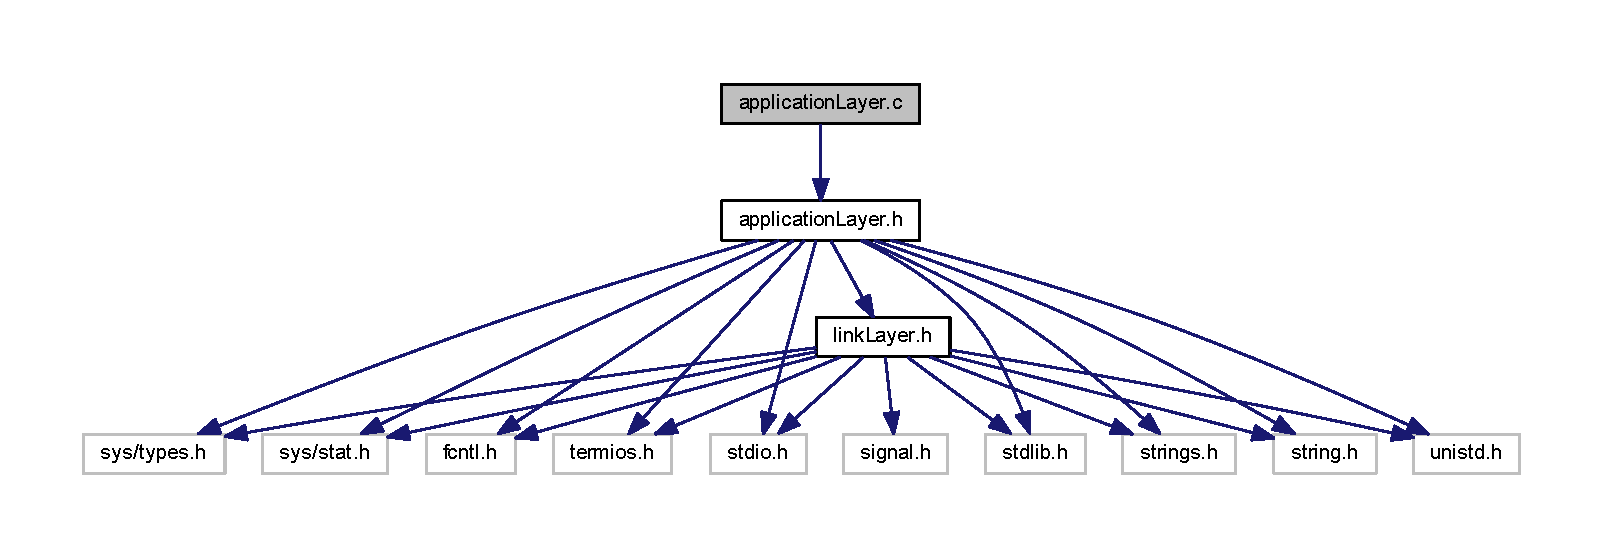
\includegraphics[width=350pt]{application_layer_8c__incl}
\end{center}
\end{figure}
\subsection*{Functions}
\begin{DoxyCompactItemize}
\item 
int \hyperlink{application_layer_8c_aa4a6846a3620f12c807f2dbd9f272298}{Init\+Application} (int file\+Descriptor, int status, char $\ast$name, int package\+Size)
\item 
int \hyperlink{application_layer_8c_a3622090a7ff391221a74cad6493bbca9}{start\+Connection} ()
\item 
int \hyperlink{application_layer_8c_a558000e1f87b3b852f73e20ba0a6b0f4}{send\+Data} ()
\item 
int \hyperlink{application_layer_8c_a73ecb47d14db1fb6e2554940364ff040}{send\+Control} (int type)
\item 
int \hyperlink{application_layer_8c_a7a2e353b862e29a450830649a7f113c9}{send\+Information} (unsigned char $\ast$buffer, int length)
\item 
int \hyperlink{application_layer_8c_a2809c0419ac7f54685983fd6d3477034}{receive\+Data} ()
\item 
int \hyperlink{application_layer_8c_a0eb8290592d5779503b7dd04fbabdb06}{receive\+Control} (int control)
\item 
int \hyperlink{application_layer_8c_a931c3be900b6917c46372f158c19022b}{receive\+Information} (unsigned char $\ast$buffer, int $\ast$length)
\item 
int \hyperlink{application_layer_8c_a0ac5863989f90535cb0fecae68437202}{show\+Receiver\+Statistics} (int num\+R\+E\+Jtransmissions, int num\+Total\+I\+Transmissions)
\item 
int \hyperlink{application_layer_8c_ab2509db0c3dc8c88c9a678df0120bc21}{show\+Transmitter\+Statistics} (int \hyperlink{link_layer_8c_a08882678e9b70455b991496b0bf0f55b}{num\+R\+E\+Jreceived}, int \hyperlink{link_layer_8c_a0637f6d853eaa5a7e5bead66bc9ee567}{num\+Frame\+Itransmitted}, int \hyperlink{link_layer_8c_ad28672c114a1578ed97b0a73abbdc761}{num\+Time\+Outs})
\end{DoxyCompactItemize}
\subsection*{Variables}
\begin{DoxyCompactItemize}
\item 
\hyperlink{struct_application_layer}{Application\+Layer} $\ast$ \hyperlink{application_layer_8c_ab8c61e9b625e569c917921aa66e15080}{app}
\item 
int \hyperlink{application_layer_8c_a423f226982e21941f55fd3d632bd810c}{frame\+Counter} = 1
\item 
int \hyperlink{application_layer_8c_a9730209d438a3addf6e04742b28c7c80}{frame\+Received} = 0
\end{DoxyCompactItemize}


\subsection{Function Documentation}
\hypertarget{application_layer_8c_aa4a6846a3620f12c807f2dbd9f272298}{}\label{application_layer_8c_aa4a6846a3620f12c807f2dbd9f272298} 
\index{application\+Layer.\+c@{application\+Layer.\+c}!Init\+Application@{Init\+Application}}
\index{Init\+Application@{Init\+Application}!application\+Layer.\+c@{application\+Layer.\+c}}
\subsubsection{\texorpdfstring{Init\+Application()}{InitApplication()}}
{\footnotesize\ttfamily int Init\+Application (\begin{DoxyParamCaption}\item[{int}]{file\+Descriptor,  }\item[{int}]{status,  }\item[{char $\ast$}]{name,  }\item[{int}]{package\+Size }\end{DoxyParamCaption})}

\mbox{[}Init\+Application description\mbox{]} 
\begin{DoxyParams}{Parameters}
{\em port} & \mbox{[}description\mbox{]} \\
\hline
{\em status} & \mbox{[}description\mbox{]} \\
\hline
{\em name} & \mbox{[}description\mbox{]} \\
\hline
{\em baud\+Rate} & \mbox{[}description\mbox{]} \\
\hline
{\em package\+Size} & \mbox{[}description\mbox{]} \\
\hline
{\em retries} & \mbox{[}description\mbox{]} \\
\hline
{\em timeout} & \mbox{[}description\mbox{]} \\
\hline
\end{DoxyParams}
\begin{DoxyReturn}{Returns}
\mbox{[}description\mbox{]} 
\end{DoxyReturn}
Here is the call graph for this function\+:
\nopagebreak
\begin{figure}[H]
\begin{center}
\leavevmode
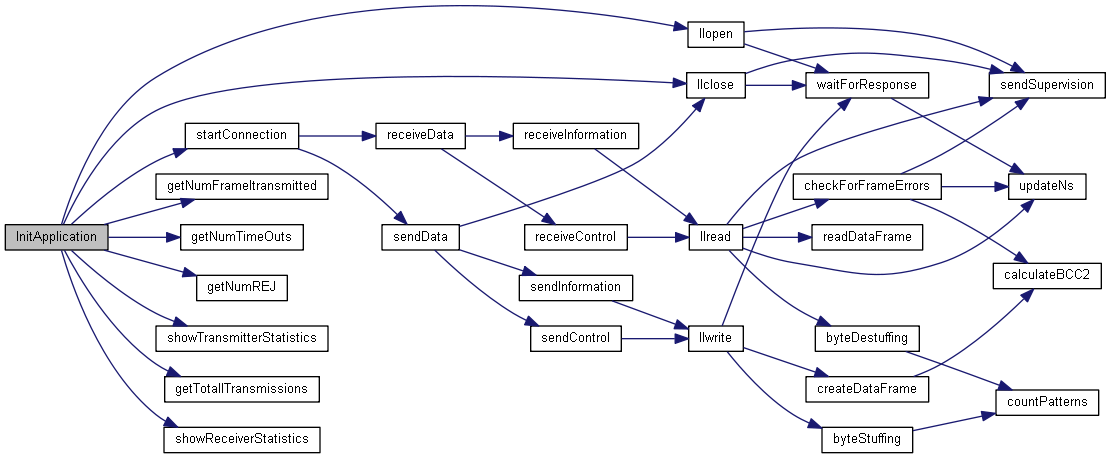
\includegraphics[width=350pt]{application_layer_8c_aa4a6846a3620f12c807f2dbd9f272298_cgraph}
\end{center}
\end{figure}
Here is the caller graph for this function\+:
\nopagebreak
\begin{figure}[H]
\begin{center}
\leavevmode
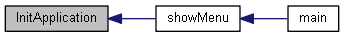
\includegraphics[width=330pt]{application_layer_8c_aa4a6846a3620f12c807f2dbd9f272298_icgraph}
\end{center}
\end{figure}
\hypertarget{application_layer_8c_a0eb8290592d5779503b7dd04fbabdb06}{}\label{application_layer_8c_a0eb8290592d5779503b7dd04fbabdb06} 
\index{application\+Layer.\+c@{application\+Layer.\+c}!receive\+Control@{receive\+Control}}
\index{receive\+Control@{receive\+Control}!application\+Layer.\+c@{application\+Layer.\+c}}
\subsubsection{\texorpdfstring{receive\+Control()}{receiveControl()}}
{\footnotesize\ttfamily int receive\+Control (\begin{DoxyParamCaption}\item[{int}]{type }\end{DoxyParamCaption})}

\mbox{[}receive\+Control description\mbox{]} 
\begin{DoxyParams}{Parameters}
{\em type} & \mbox{[}description\mbox{]} \\
\hline
\end{DoxyParams}
\begin{DoxyReturn}{Returns}
\mbox{[}description\mbox{]} 
\end{DoxyReturn}
Here is the call graph for this function\+:
\nopagebreak
\begin{figure}[H]
\begin{center}
\leavevmode
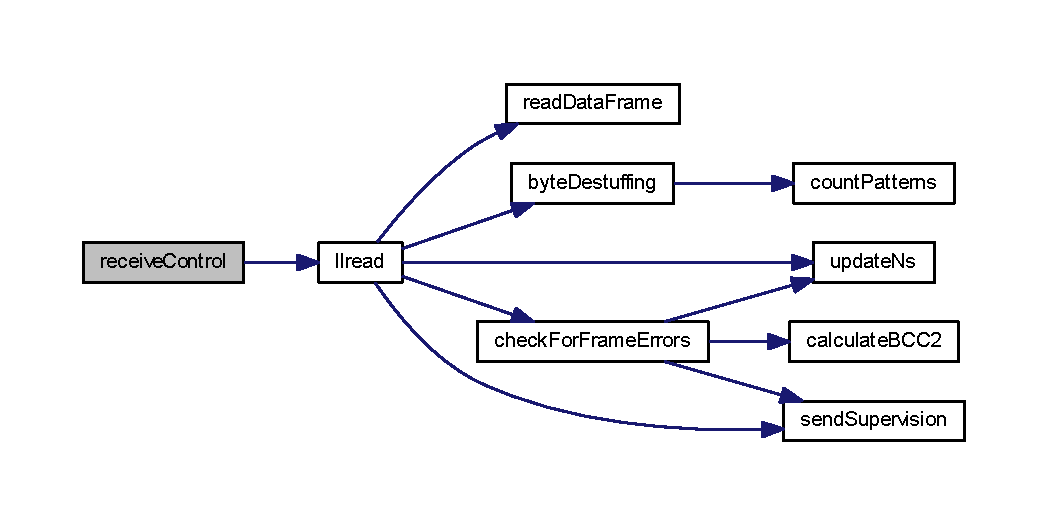
\includegraphics[width=350pt]{application_layer_8c_a0eb8290592d5779503b7dd04fbabdb06_cgraph}
\end{center}
\end{figure}
Here is the caller graph for this function\+:
\nopagebreak
\begin{figure}[H]
\begin{center}
\leavevmode
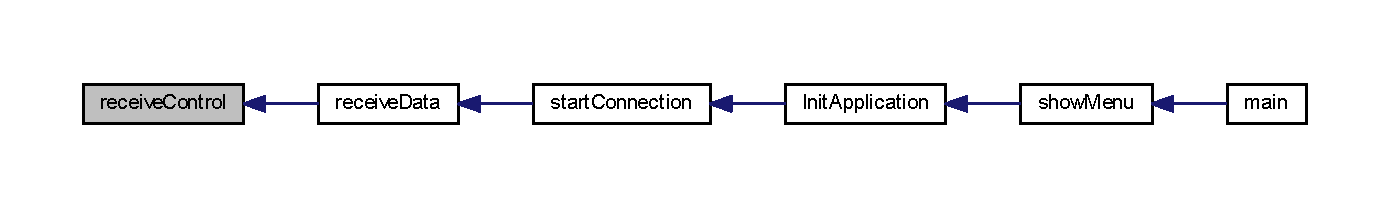
\includegraphics[width=350pt]{application_layer_8c_a0eb8290592d5779503b7dd04fbabdb06_icgraph}
\end{center}
\end{figure}
\hypertarget{application_layer_8c_a2809c0419ac7f54685983fd6d3477034}{}\label{application_layer_8c_a2809c0419ac7f54685983fd6d3477034} 
\index{application\+Layer.\+c@{application\+Layer.\+c}!receive\+Data@{receive\+Data}}
\index{receive\+Data@{receive\+Data}!application\+Layer.\+c@{application\+Layer.\+c}}
\subsubsection{\texorpdfstring{receive\+Data()}{receiveData()}}
{\footnotesize\ttfamily int receive\+Data (\begin{DoxyParamCaption}{ }\end{DoxyParamCaption})}

\mbox{[}receive\+Data description\mbox{]} \begin{DoxyReturn}{Returns}
\mbox{[}description\mbox{]} 
\end{DoxyReturn}
Here is the call graph for this function\+:
\nopagebreak
\begin{figure}[H]
\begin{center}
\leavevmode
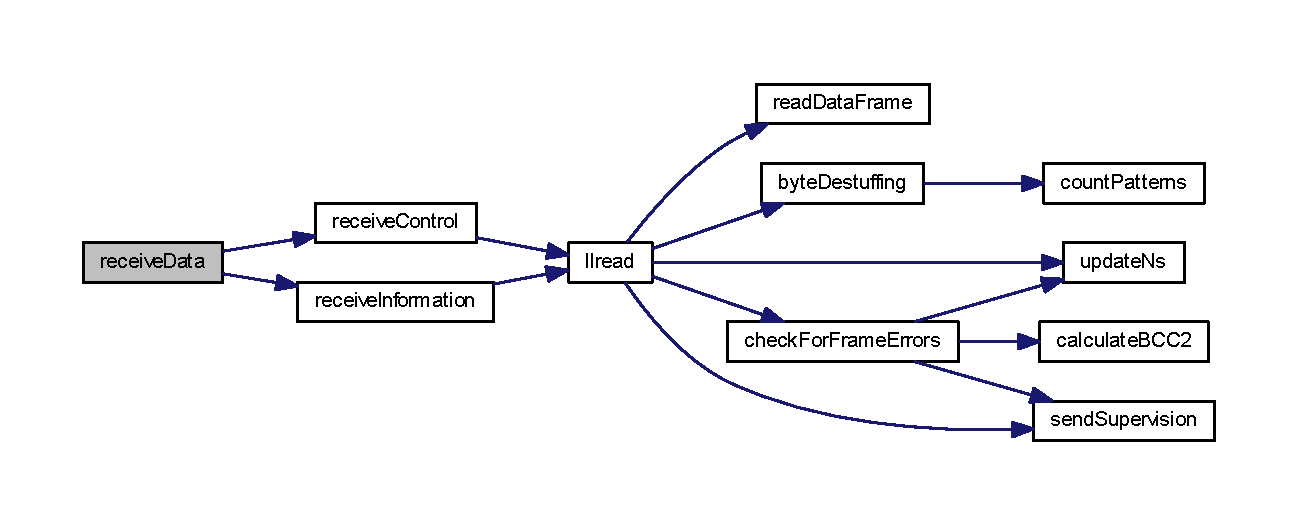
\includegraphics[width=350pt]{application_layer_8c_a2809c0419ac7f54685983fd6d3477034_cgraph}
\end{center}
\end{figure}
Here is the caller graph for this function\+:
\nopagebreak
\begin{figure}[H]
\begin{center}
\leavevmode
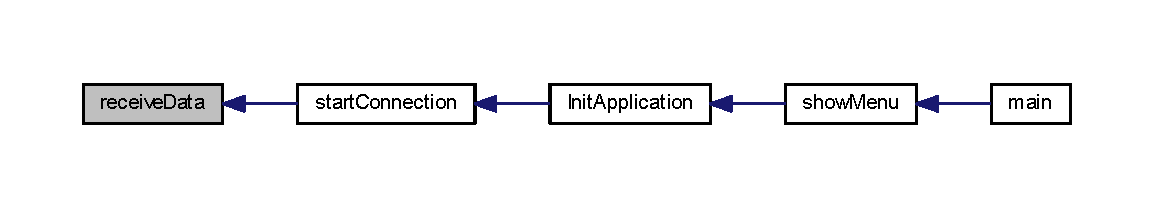
\includegraphics[width=350pt]{application_layer_8c_a2809c0419ac7f54685983fd6d3477034_icgraph}
\end{center}
\end{figure}
\hypertarget{application_layer_8c_a931c3be900b6917c46372f158c19022b}{}\label{application_layer_8c_a931c3be900b6917c46372f158c19022b} 
\index{application\+Layer.\+c@{application\+Layer.\+c}!receive\+Information@{receive\+Information}}
\index{receive\+Information@{receive\+Information}!application\+Layer.\+c@{application\+Layer.\+c}}
\subsubsection{\texorpdfstring{receive\+Information()}{receiveInformation()}}
{\footnotesize\ttfamily int receive\+Information (\begin{DoxyParamCaption}\item[{unsigned char $\ast$}]{buffer,  }\item[{int $\ast$}]{length }\end{DoxyParamCaption})}

\mbox{[}receive\+Information description\mbox{]} 
\begin{DoxyParams}{Parameters}
{\em buffer} & \mbox{[}description\mbox{]} \\
\hline
{\em length} & \mbox{[}description\mbox{]} \\
\hline
\end{DoxyParams}
\begin{DoxyReturn}{Returns}
\mbox{[}description\mbox{]} 
\end{DoxyReturn}
Here is the call graph for this function\+:
\nopagebreak
\begin{figure}[H]
\begin{center}
\leavevmode
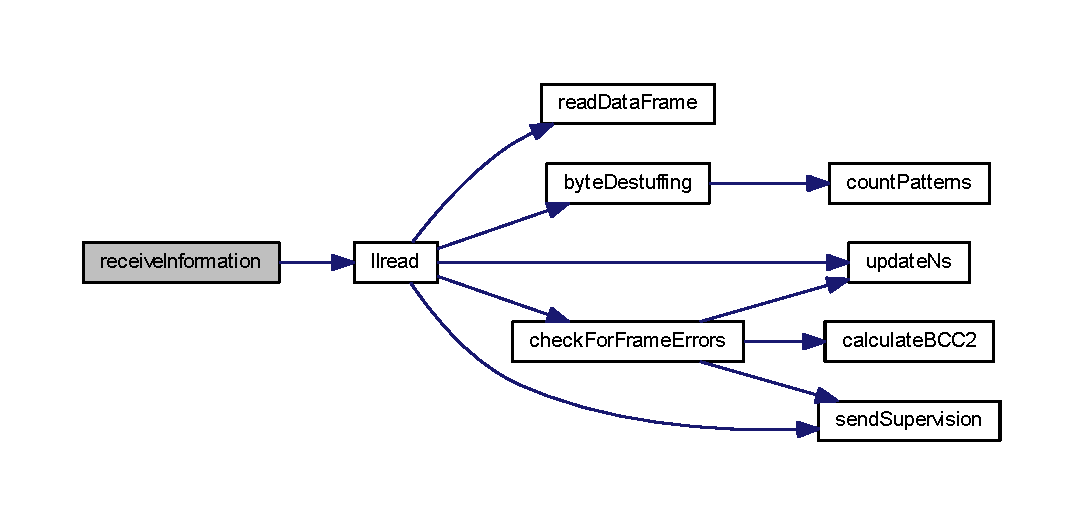
\includegraphics[width=350pt]{application_layer_8c_a931c3be900b6917c46372f158c19022b_cgraph}
\end{center}
\end{figure}
Here is the caller graph for this function\+:
\nopagebreak
\begin{figure}[H]
\begin{center}
\leavevmode
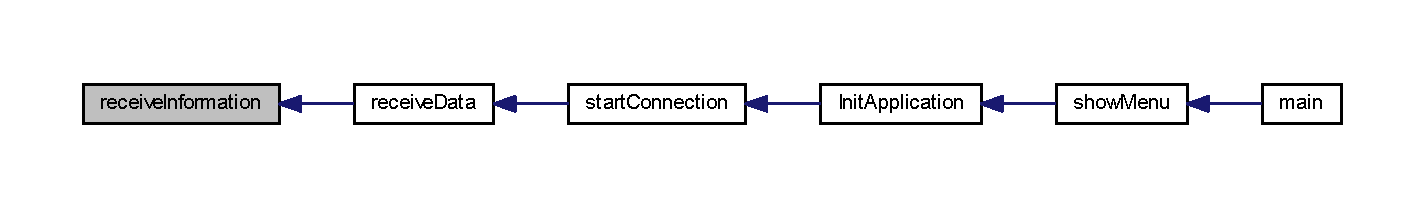
\includegraphics[width=350pt]{application_layer_8c_a931c3be900b6917c46372f158c19022b_icgraph}
\end{center}
\end{figure}
\hypertarget{application_layer_8c_a73ecb47d14db1fb6e2554940364ff040}{}\label{application_layer_8c_a73ecb47d14db1fb6e2554940364ff040} 
\index{application\+Layer.\+c@{application\+Layer.\+c}!send\+Control@{send\+Control}}
\index{send\+Control@{send\+Control}!application\+Layer.\+c@{application\+Layer.\+c}}
\subsubsection{\texorpdfstring{send\+Control()}{sendControl()}}
{\footnotesize\ttfamily int send\+Control (\begin{DoxyParamCaption}\item[{int}]{type }\end{DoxyParamCaption})}

\mbox{[}send\+Control description\mbox{]} 
\begin{DoxyParams}{Parameters}
{\em type} & \mbox{[}description\mbox{]} \\
\hline
\end{DoxyParams}
\begin{DoxyReturn}{Returns}
\mbox{[}description\mbox{]} 
\end{DoxyReturn}
Here is the call graph for this function\+:
\nopagebreak
\begin{figure}[H]
\begin{center}
\leavevmode
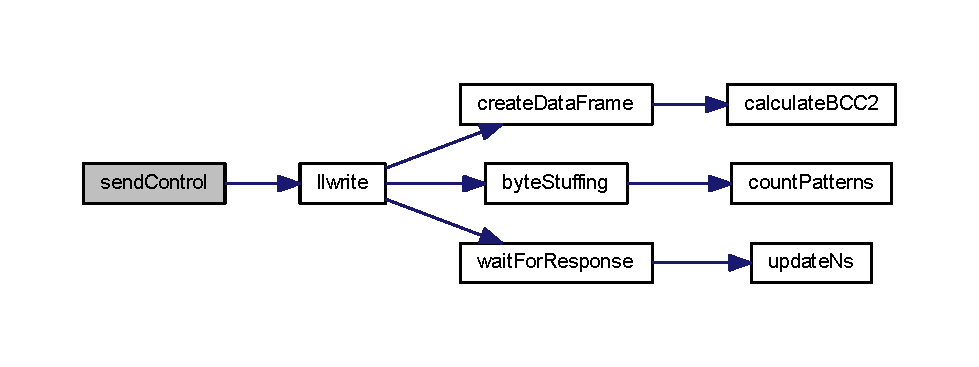
\includegraphics[width=350pt]{application_layer_8c_a73ecb47d14db1fb6e2554940364ff040_cgraph}
\end{center}
\end{figure}
Here is the caller graph for this function\+:
\nopagebreak
\begin{figure}[H]
\begin{center}
\leavevmode
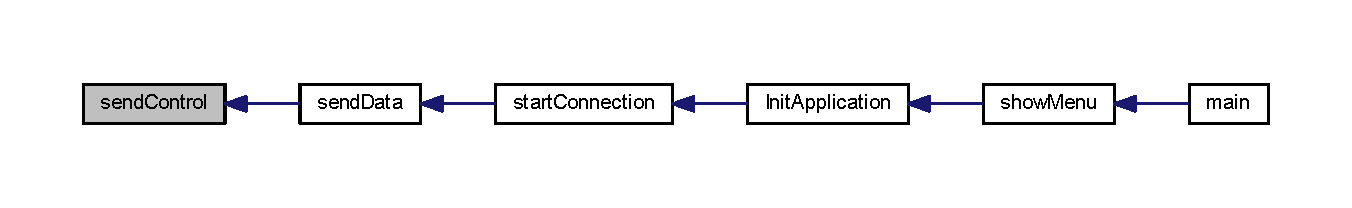
\includegraphics[width=350pt]{application_layer_8c_a73ecb47d14db1fb6e2554940364ff040_icgraph}
\end{center}
\end{figure}
\hypertarget{application_layer_8c_a558000e1f87b3b852f73e20ba0a6b0f4}{}\label{application_layer_8c_a558000e1f87b3b852f73e20ba0a6b0f4} 
\index{application\+Layer.\+c@{application\+Layer.\+c}!send\+Data@{send\+Data}}
\index{send\+Data@{send\+Data}!application\+Layer.\+c@{application\+Layer.\+c}}
\subsubsection{\texorpdfstring{send\+Data()}{sendData()}}
{\footnotesize\ttfamily int send\+Data (\begin{DoxyParamCaption}{ }\end{DoxyParamCaption})}

\mbox{[}send\+Data description\mbox{]} \begin{DoxyReturn}{Returns}
\mbox{[}description\mbox{]} 
\end{DoxyReturn}
Here is the call graph for this function\+:
\nopagebreak
\begin{figure}[H]
\begin{center}
\leavevmode
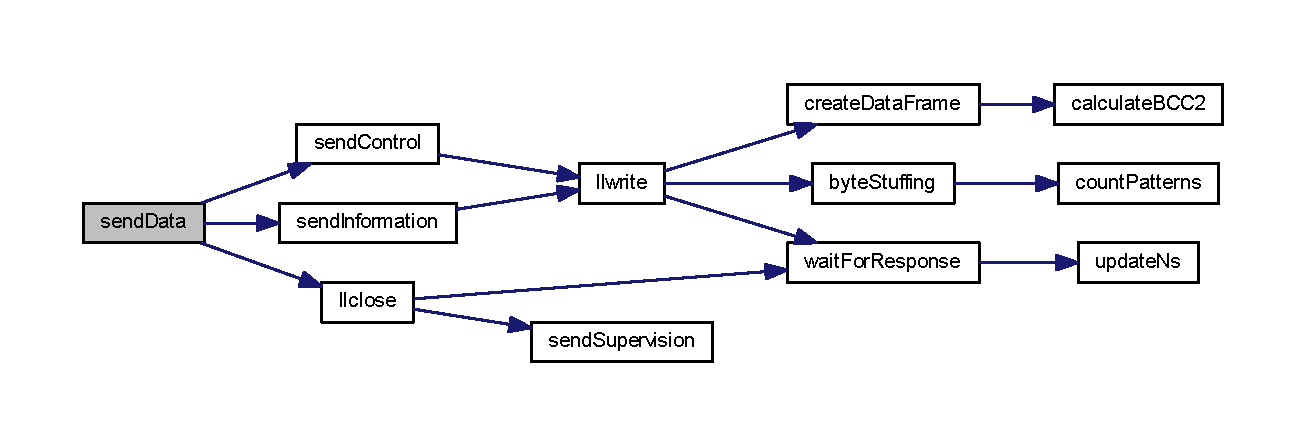
\includegraphics[width=350pt]{application_layer_8c_a558000e1f87b3b852f73e20ba0a6b0f4_cgraph}
\end{center}
\end{figure}
Here is the caller graph for this function\+:
\nopagebreak
\begin{figure}[H]
\begin{center}
\leavevmode
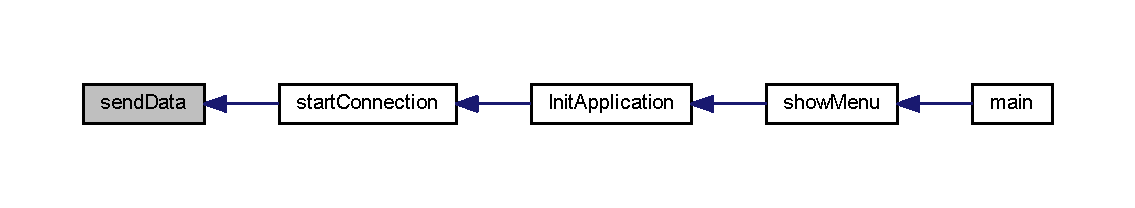
\includegraphics[width=350pt]{application_layer_8c_a558000e1f87b3b852f73e20ba0a6b0f4_icgraph}
\end{center}
\end{figure}
\hypertarget{application_layer_8c_a7a2e353b862e29a450830649a7f113c9}{}\label{application_layer_8c_a7a2e353b862e29a450830649a7f113c9} 
\index{application\+Layer.\+c@{application\+Layer.\+c}!send\+Information@{send\+Information}}
\index{send\+Information@{send\+Information}!application\+Layer.\+c@{application\+Layer.\+c}}
\subsubsection{\texorpdfstring{send\+Information()}{sendInformation()}}
{\footnotesize\ttfamily int send\+Information (\begin{DoxyParamCaption}\item[{unsigned char $\ast$}]{buffer,  }\item[{int}]{length }\end{DoxyParamCaption})}

\mbox{[}send\+Information description\mbox{]} 
\begin{DoxyParams}{Parameters}
{\em buffer} & \mbox{[}description\mbox{]} \\
\hline
{\em length} & \mbox{[}description\mbox{]} \\
\hline
\end{DoxyParams}
\begin{DoxyReturn}{Returns}
\mbox{[}description\mbox{]} 
\end{DoxyReturn}
Here is the call graph for this function\+:
\nopagebreak
\begin{figure}[H]
\begin{center}
\leavevmode
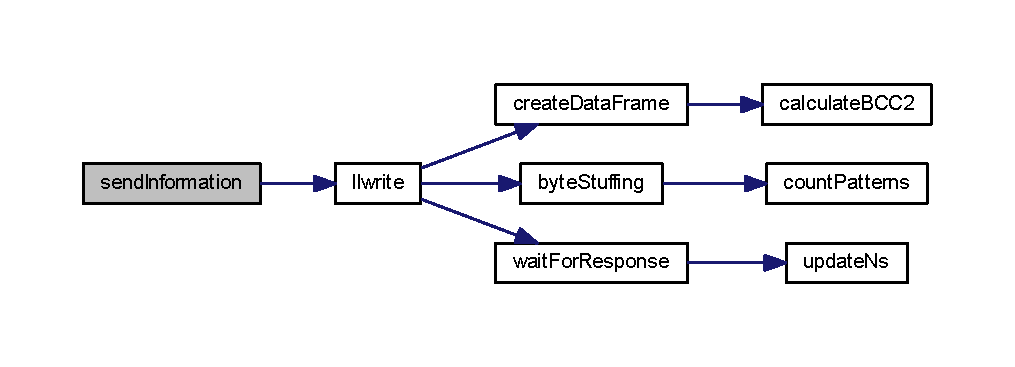
\includegraphics[width=350pt]{application_layer_8c_a7a2e353b862e29a450830649a7f113c9_cgraph}
\end{center}
\end{figure}
Here is the caller graph for this function\+:
\nopagebreak
\begin{figure}[H]
\begin{center}
\leavevmode
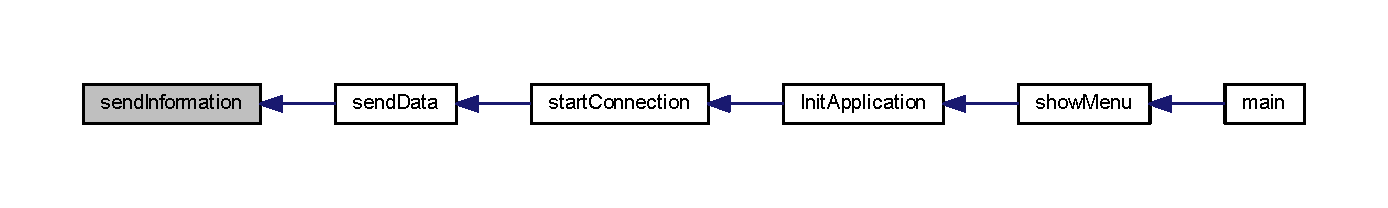
\includegraphics[width=350pt]{application_layer_8c_a7a2e353b862e29a450830649a7f113c9_icgraph}
\end{center}
\end{figure}
\hypertarget{application_layer_8c_a0ac5863989f90535cb0fecae68437202}{}\label{application_layer_8c_a0ac5863989f90535cb0fecae68437202} 
\index{application\+Layer.\+c@{application\+Layer.\+c}!show\+Receiver\+Statistics@{show\+Receiver\+Statistics}}
\index{show\+Receiver\+Statistics@{show\+Receiver\+Statistics}!application\+Layer.\+c@{application\+Layer.\+c}}
\subsubsection{\texorpdfstring{show\+Receiver\+Statistics()}{showReceiverStatistics()}}
{\footnotesize\ttfamily int show\+Receiver\+Statistics (\begin{DoxyParamCaption}\item[{int}]{num\+R\+E\+Jtransmissions,  }\item[{int}]{num\+Total\+I\+Transmissions }\end{DoxyParamCaption})}

Here is the caller graph for this function\+:
\nopagebreak
\begin{figure}[H]
\begin{center}
\leavevmode
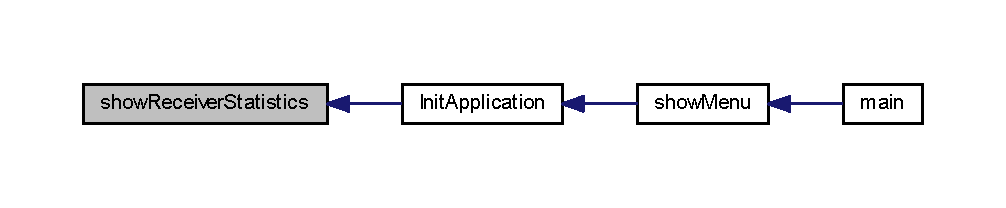
\includegraphics[width=350pt]{application_layer_8c_a0ac5863989f90535cb0fecae68437202_icgraph}
\end{center}
\end{figure}
\hypertarget{application_layer_8c_ab2509db0c3dc8c88c9a678df0120bc21}{}\label{application_layer_8c_ab2509db0c3dc8c88c9a678df0120bc21} 
\index{application\+Layer.\+c@{application\+Layer.\+c}!show\+Transmitter\+Statistics@{show\+Transmitter\+Statistics}}
\index{show\+Transmitter\+Statistics@{show\+Transmitter\+Statistics}!application\+Layer.\+c@{application\+Layer.\+c}}
\subsubsection{\texorpdfstring{show\+Transmitter\+Statistics()}{showTransmitterStatistics()}}
{\footnotesize\ttfamily int show\+Transmitter\+Statistics (\begin{DoxyParamCaption}\item[{int}]{num\+R\+E\+Jreceived,  }\item[{int}]{num\+Frame\+Itransmitted,  }\item[{int}]{num\+Time\+Outs }\end{DoxyParamCaption})}

Here is the caller graph for this function\+:
\nopagebreak
\begin{figure}[H]
\begin{center}
\leavevmode
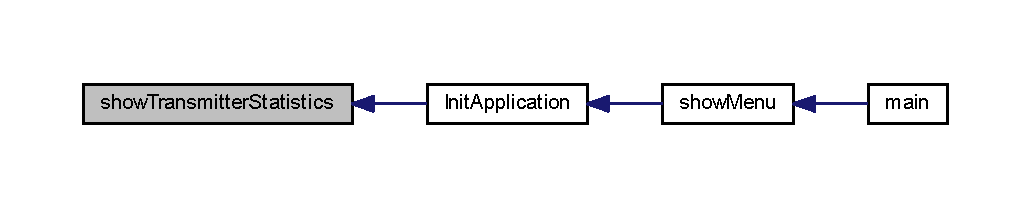
\includegraphics[width=350pt]{application_layer_8c_ab2509db0c3dc8c88c9a678df0120bc21_icgraph}
\end{center}
\end{figure}
\hypertarget{application_layer_8c_a3622090a7ff391221a74cad6493bbca9}{}\label{application_layer_8c_a3622090a7ff391221a74cad6493bbca9} 
\index{application\+Layer.\+c@{application\+Layer.\+c}!start\+Connection@{start\+Connection}}
\index{start\+Connection@{start\+Connection}!application\+Layer.\+c@{application\+Layer.\+c}}
\subsubsection{\texorpdfstring{start\+Connection()}{startConnection()}}
{\footnotesize\ttfamily int start\+Connection (\begin{DoxyParamCaption}{ }\end{DoxyParamCaption})}

\mbox{[}start\+Connection description\mbox{]} \begin{DoxyReturn}{Returns}
\mbox{[}description\mbox{]} 
\end{DoxyReturn}
Here is the call graph for this function\+:
\nopagebreak
\begin{figure}[H]
\begin{center}
\leavevmode
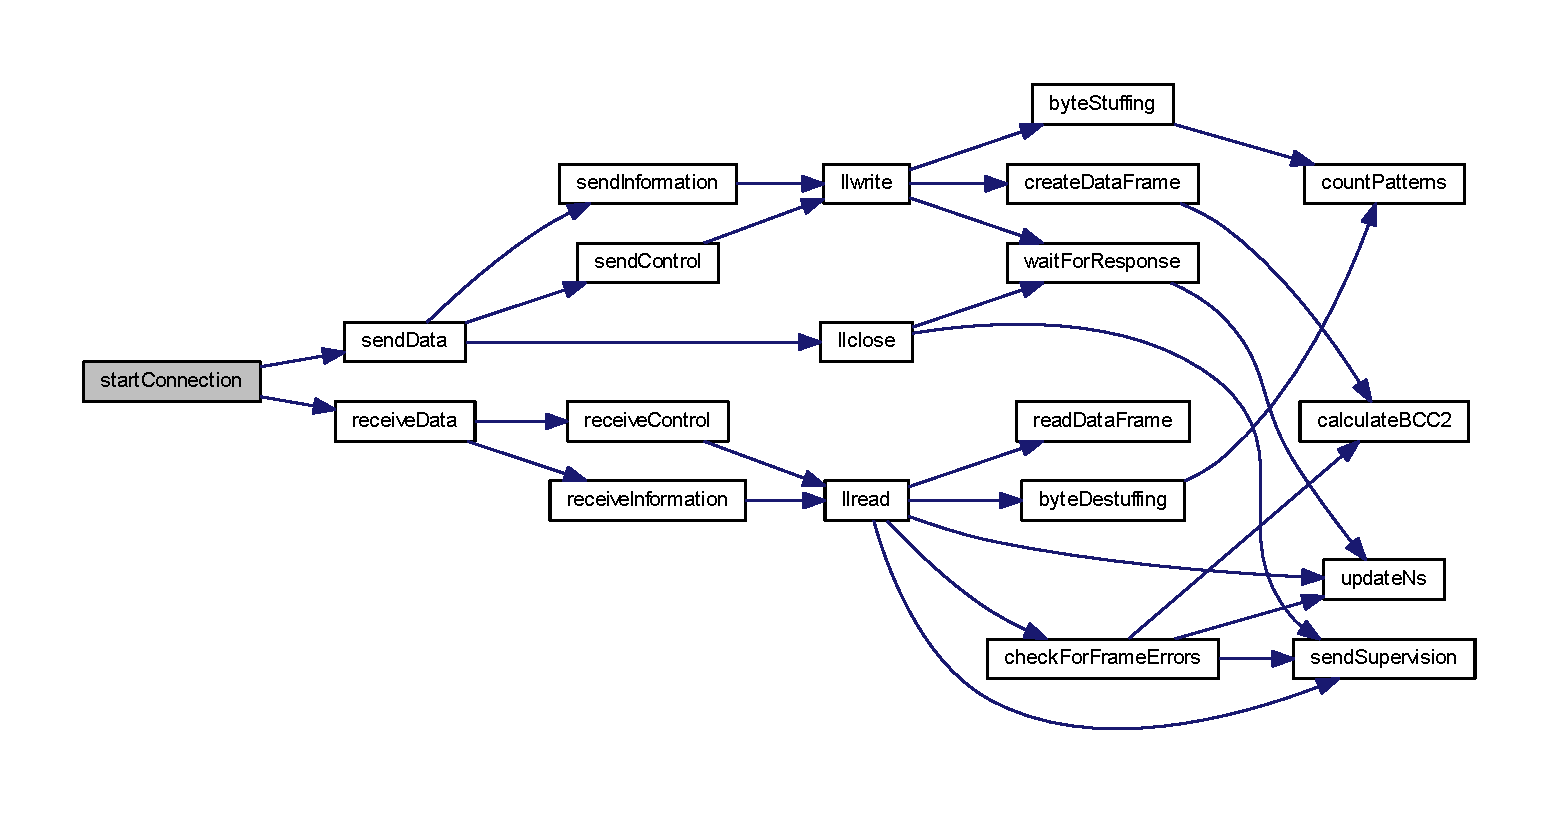
\includegraphics[width=350pt]{application_layer_8c_a3622090a7ff391221a74cad6493bbca9_cgraph}
\end{center}
\end{figure}
Here is the caller graph for this function\+:
\nopagebreak
\begin{figure}[H]
\begin{center}
\leavevmode
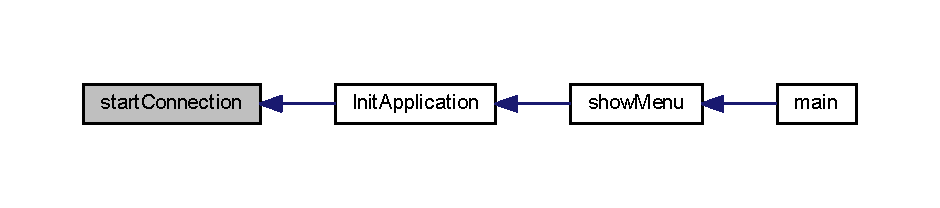
\includegraphics[width=350pt]{application_layer_8c_a3622090a7ff391221a74cad6493bbca9_icgraph}
\end{center}
\end{figure}


\subsection{Variable Documentation}
\hypertarget{application_layer_8c_ab8c61e9b625e569c917921aa66e15080}{}\label{application_layer_8c_ab8c61e9b625e569c917921aa66e15080} 
\index{application\+Layer.\+c@{application\+Layer.\+c}!app@{app}}
\index{app@{app}!application\+Layer.\+c@{application\+Layer.\+c}}
\subsubsection{\texorpdfstring{app}{app}}
{\footnotesize\ttfamily \hyperlink{struct_application_layer}{Application\+Layer}$\ast$ app}

\hypertarget{application_layer_8c_a423f226982e21941f55fd3d632bd810c}{}\label{application_layer_8c_a423f226982e21941f55fd3d632bd810c} 
\index{application\+Layer.\+c@{application\+Layer.\+c}!frame\+Counter@{frame\+Counter}}
\index{frame\+Counter@{frame\+Counter}!application\+Layer.\+c@{application\+Layer.\+c}}
\subsubsection{\texorpdfstring{frame\+Counter}{frameCounter}}
{\footnotesize\ttfamily int frame\+Counter = 1}

\hypertarget{application_layer_8c_a9730209d438a3addf6e04742b28c7c80}{}\label{application_layer_8c_a9730209d438a3addf6e04742b28c7c80} 
\index{application\+Layer.\+c@{application\+Layer.\+c}!frame\+Received@{frame\+Received}}
\index{frame\+Received@{frame\+Received}!application\+Layer.\+c@{application\+Layer.\+c}}
\subsubsection{\texorpdfstring{frame\+Received}{frameReceived}}
{\footnotesize\ttfamily int frame\+Received = 0}


\hypertarget{application_layer_8h}{}\section{application\+Layer.\+h File Reference}
\label{application_layer_8h}\index{application\+Layer.\+h@{application\+Layer.\+h}}
{\ttfamily \#include $<$sys/types.\+h$>$}\newline
{\ttfamily \#include $<$sys/stat.\+h$>$}\newline
{\ttfamily \#include $<$fcntl.\+h$>$}\newline
{\ttfamily \#include $<$termios.\+h$>$}\newline
{\ttfamily \#include $<$stdio.\+h$>$}\newline
{\ttfamily \#include $<$stdlib.\+h$>$}\newline
{\ttfamily \#include $<$strings.\+h$>$}\newline
{\ttfamily \#include $<$string.\+h$>$}\newline
{\ttfamily \#include $<$unistd.\+h$>$}\newline
{\ttfamily \#include \char`\"{}link\+Layer.\+h\char`\"{}}\newline
Include dependency graph for application\+Layer.\+h\+:\nopagebreak
\begin{figure}[H]
\begin{center}
\leavevmode
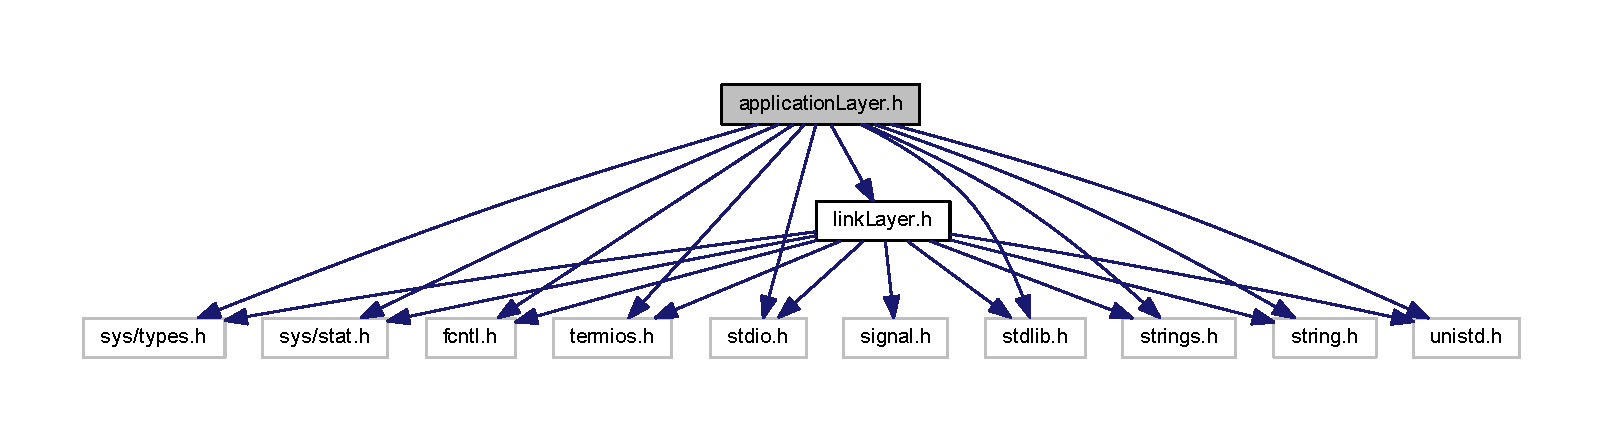
\includegraphics[width=350pt]{application_layer_8h__incl}
\end{center}
\end{figure}
This graph shows which files directly or indirectly include this file\+:\nopagebreak
\begin{figure}[H]
\begin{center}
\leavevmode
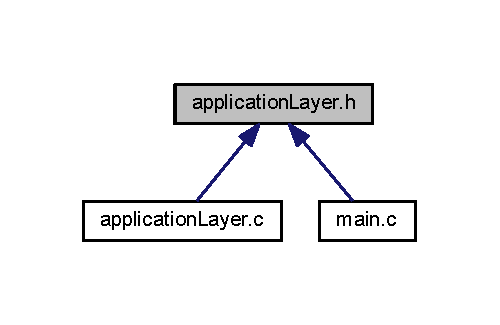
\includegraphics[width=240pt]{application_layer_8h__dep__incl}
\end{center}
\end{figure}
\subsection*{Data Structures}
\begin{DoxyCompactItemize}
\item 
struct \hyperlink{struct_application_layer}{Application\+Layer}
\end{DoxyCompactItemize}
\subsection*{Macros}
\begin{DoxyCompactItemize}
\item 
\#define \hyperlink{application_layer_8h_abf940742e1b38f8100a344f9275d4086}{B\+U\+F\+\_\+\+M\+AX}~255
\item 
\#define \hyperlink{application_layer_8h_a2f79666675d7ae9fdfdb3a825ef55d5a}{C\+O\+N\+T\+R\+O\+L\+\_\+\+D\+A\+TA}~0x01
\item 
\#define \hyperlink{application_layer_8h_ab3a620b0bd8e67f0942ba85c71c094bb}{C\+O\+N\+T\+R\+O\+L\+\_\+\+S\+T\+A\+RT}~0x02
\item 
\#define \hyperlink{application_layer_8h_abaab712c949e54f62908fddc254e46b1}{C\+O\+N\+T\+R\+O\+L\+\_\+\+E\+ND}~0x03
\item 
\#define \hyperlink{application_layer_8h_af3c3df6c9906ede8f09fa2af74cb28d5}{F\+I\+L\+E\+\_\+\+S\+I\+ZE}~0x00
\item 
\#define \hyperlink{application_layer_8h_ab117546549783a058d0321a287699579}{F\+I\+L\+E\+\_\+\+N\+A\+ME}~0x01
\item 
\#define \hyperlink{application_layer_8h_a5b5ca0ae07e92e9cad54568049f06fce}{Data\+Headers}~4
\item 
\#define \hyperlink{application_layer_8h_ab983f03862f557a786ccc43b26522e16}{L2}~0x00
\item 
\#define \hyperlink{application_layer_8h_a455948b8bd5f5ce920899ae1013c4b4c}{R\+E\+C\+E\+I\+V\+ER}~1
\item 
\#define \hyperlink{application_layer_8h_a4dd2cc1f618201244956369378b75c9a}{T\+R\+A\+N\+S\+M\+I\+T\+T\+ER}~0
\end{DoxyCompactItemize}
\subsection*{Typedefs}
\begin{DoxyCompactItemize}
\item 
typedef struct \hyperlink{struct_application_layer}{Application\+Layer} \hyperlink{application_layer_8h_acaaa4243674fb079f4d233d17759f36b}{Application\+Layer}
\end{DoxyCompactItemize}
\subsection*{Functions}
\begin{DoxyCompactItemize}
\item 
int \hyperlink{application_layer_8h_abdd55a6320cd4fbce91a0583d4ad05f5}{Init\+Application} (int port, int status, char $\ast$name, int \hyperlink{main_8c_a352a05efbed742a2c47e738725ee5613}{baud\+Rate}, int package\+Size, int \hyperlink{main_8c_a8ba735ab56b2afeb844916994c86f3f5}{retries}, int timeout)
\item 
int \hyperlink{application_layer_8h_a3622090a7ff391221a74cad6493bbca9}{start\+Connection} ()
\item 
int \hyperlink{application_layer_8h_a558000e1f87b3b852f73e20ba0a6b0f4}{send\+Data} ()
\item 
int \hyperlink{application_layer_8h_a73ecb47d14db1fb6e2554940364ff040}{send\+Control} (int type)
\item 
int \hyperlink{application_layer_8h_a7a2e353b862e29a450830649a7f113c9}{send\+Information} (unsigned char $\ast$buffer, int length)
\item 
int \hyperlink{application_layer_8h_a2809c0419ac7f54685983fd6d3477034}{receive\+Data} ()
\item 
int \hyperlink{application_layer_8h_a631126e029a493e74a1af5aacf2a7c16}{receive\+Control} (int type)
\item 
int \hyperlink{application_layer_8h_a931c3be900b6917c46372f158c19022b}{receive\+Information} (unsigned char $\ast$buffer, int $\ast$length)
\item 
int \hyperlink{application_layer_8h_a0ac5863989f90535cb0fecae68437202}{show\+Receiver\+Statistics} (int num\+R\+E\+Jtransmissions, int num\+Total\+I\+Transmissions)
\item 
int \hyperlink{application_layer_8h_ab2509db0c3dc8c88c9a678df0120bc21}{show\+Transmitter\+Statistics} (int \hyperlink{link_layer_8c_a08882678e9b70455b991496b0bf0f55b}{num\+R\+E\+Jreceived}, int \hyperlink{link_layer_8c_a0637f6d853eaa5a7e5bead66bc9ee567}{num\+Frame\+Itransmitted}, int \hyperlink{link_layer_8c_ad28672c114a1578ed97b0a73abbdc761}{num\+Time\+Outs})
\end{DoxyCompactItemize}


\subsection{Macro Definition Documentation}
\hypertarget{application_layer_8h_abf940742e1b38f8100a344f9275d4086}{}\label{application_layer_8h_abf940742e1b38f8100a344f9275d4086} 
\index{application\+Layer.\+h@{application\+Layer.\+h}!B\+U\+F\+\_\+\+M\+AX@{B\+U\+F\+\_\+\+M\+AX}}
\index{B\+U\+F\+\_\+\+M\+AX@{B\+U\+F\+\_\+\+M\+AX}!application\+Layer.\+h@{application\+Layer.\+h}}
\subsubsection{\texorpdfstring{B\+U\+F\+\_\+\+M\+AX}{BUF\_MAX}}
{\footnotesize\ttfamily \#define B\+U\+F\+\_\+\+M\+AX~255}

\hypertarget{application_layer_8h_a2f79666675d7ae9fdfdb3a825ef55d5a}{}\label{application_layer_8h_a2f79666675d7ae9fdfdb3a825ef55d5a} 
\index{application\+Layer.\+h@{application\+Layer.\+h}!C\+O\+N\+T\+R\+O\+L\+\_\+\+D\+A\+TA@{C\+O\+N\+T\+R\+O\+L\+\_\+\+D\+A\+TA}}
\index{C\+O\+N\+T\+R\+O\+L\+\_\+\+D\+A\+TA@{C\+O\+N\+T\+R\+O\+L\+\_\+\+D\+A\+TA}!application\+Layer.\+h@{application\+Layer.\+h}}
\subsubsection{\texorpdfstring{C\+O\+N\+T\+R\+O\+L\+\_\+\+D\+A\+TA}{CONTROL\_DATA}}
{\footnotesize\ttfamily \#define C\+O\+N\+T\+R\+O\+L\+\_\+\+D\+A\+TA~0x01}

\hypertarget{application_layer_8h_abaab712c949e54f62908fddc254e46b1}{}\label{application_layer_8h_abaab712c949e54f62908fddc254e46b1} 
\index{application\+Layer.\+h@{application\+Layer.\+h}!C\+O\+N\+T\+R\+O\+L\+\_\+\+E\+ND@{C\+O\+N\+T\+R\+O\+L\+\_\+\+E\+ND}}
\index{C\+O\+N\+T\+R\+O\+L\+\_\+\+E\+ND@{C\+O\+N\+T\+R\+O\+L\+\_\+\+E\+ND}!application\+Layer.\+h@{application\+Layer.\+h}}
\subsubsection{\texorpdfstring{C\+O\+N\+T\+R\+O\+L\+\_\+\+E\+ND}{CONTROL\_END}}
{\footnotesize\ttfamily \#define C\+O\+N\+T\+R\+O\+L\+\_\+\+E\+ND~0x03}

\hypertarget{application_layer_8h_ab3a620b0bd8e67f0942ba85c71c094bb}{}\label{application_layer_8h_ab3a620b0bd8e67f0942ba85c71c094bb} 
\index{application\+Layer.\+h@{application\+Layer.\+h}!C\+O\+N\+T\+R\+O\+L\+\_\+\+S\+T\+A\+RT@{C\+O\+N\+T\+R\+O\+L\+\_\+\+S\+T\+A\+RT}}
\index{C\+O\+N\+T\+R\+O\+L\+\_\+\+S\+T\+A\+RT@{C\+O\+N\+T\+R\+O\+L\+\_\+\+S\+T\+A\+RT}!application\+Layer.\+h@{application\+Layer.\+h}}
\subsubsection{\texorpdfstring{C\+O\+N\+T\+R\+O\+L\+\_\+\+S\+T\+A\+RT}{CONTROL\_START}}
{\footnotesize\ttfamily \#define C\+O\+N\+T\+R\+O\+L\+\_\+\+S\+T\+A\+RT~0x02}

\hypertarget{application_layer_8h_a5b5ca0ae07e92e9cad54568049f06fce}{}\label{application_layer_8h_a5b5ca0ae07e92e9cad54568049f06fce} 
\index{application\+Layer.\+h@{application\+Layer.\+h}!Data\+Headers@{Data\+Headers}}
\index{Data\+Headers@{Data\+Headers}!application\+Layer.\+h@{application\+Layer.\+h}}
\subsubsection{\texorpdfstring{Data\+Headers}{DataHeaders}}
{\footnotesize\ttfamily \#define Data\+Headers~4}

\hypertarget{application_layer_8h_ab117546549783a058d0321a287699579}{}\label{application_layer_8h_ab117546549783a058d0321a287699579} 
\index{application\+Layer.\+h@{application\+Layer.\+h}!F\+I\+L\+E\+\_\+\+N\+A\+ME@{F\+I\+L\+E\+\_\+\+N\+A\+ME}}
\index{F\+I\+L\+E\+\_\+\+N\+A\+ME@{F\+I\+L\+E\+\_\+\+N\+A\+ME}!application\+Layer.\+h@{application\+Layer.\+h}}
\subsubsection{\texorpdfstring{F\+I\+L\+E\+\_\+\+N\+A\+ME}{FILE\_NAME}}
{\footnotesize\ttfamily \#define F\+I\+L\+E\+\_\+\+N\+A\+ME~0x01}

\hypertarget{application_layer_8h_af3c3df6c9906ede8f09fa2af74cb28d5}{}\label{application_layer_8h_af3c3df6c9906ede8f09fa2af74cb28d5} 
\index{application\+Layer.\+h@{application\+Layer.\+h}!F\+I\+L\+E\+\_\+\+S\+I\+ZE@{F\+I\+L\+E\+\_\+\+S\+I\+ZE}}
\index{F\+I\+L\+E\+\_\+\+S\+I\+ZE@{F\+I\+L\+E\+\_\+\+S\+I\+ZE}!application\+Layer.\+h@{application\+Layer.\+h}}
\subsubsection{\texorpdfstring{F\+I\+L\+E\+\_\+\+S\+I\+ZE}{FILE\_SIZE}}
{\footnotesize\ttfamily \#define F\+I\+L\+E\+\_\+\+S\+I\+ZE~0x00}

\hypertarget{application_layer_8h_ab983f03862f557a786ccc43b26522e16}{}\label{application_layer_8h_ab983f03862f557a786ccc43b26522e16} 
\index{application\+Layer.\+h@{application\+Layer.\+h}!L2@{L2}}
\index{L2@{L2}!application\+Layer.\+h@{application\+Layer.\+h}}
\subsubsection{\texorpdfstring{L2}{L2}}
{\footnotesize\ttfamily \#define L2~0x00}

\hypertarget{application_layer_8h_a455948b8bd5f5ce920899ae1013c4b4c}{}\label{application_layer_8h_a455948b8bd5f5ce920899ae1013c4b4c} 
\index{application\+Layer.\+h@{application\+Layer.\+h}!R\+E\+C\+E\+I\+V\+ER@{R\+E\+C\+E\+I\+V\+ER}}
\index{R\+E\+C\+E\+I\+V\+ER@{R\+E\+C\+E\+I\+V\+ER}!application\+Layer.\+h@{application\+Layer.\+h}}
\subsubsection{\texorpdfstring{R\+E\+C\+E\+I\+V\+ER}{RECEIVER}}
{\footnotesize\ttfamily \#define R\+E\+C\+E\+I\+V\+ER~1}

\hypertarget{application_layer_8h_a4dd2cc1f618201244956369378b75c9a}{}\label{application_layer_8h_a4dd2cc1f618201244956369378b75c9a} 
\index{application\+Layer.\+h@{application\+Layer.\+h}!T\+R\+A\+N\+S\+M\+I\+T\+T\+ER@{T\+R\+A\+N\+S\+M\+I\+T\+T\+ER}}
\index{T\+R\+A\+N\+S\+M\+I\+T\+T\+ER@{T\+R\+A\+N\+S\+M\+I\+T\+T\+ER}!application\+Layer.\+h@{application\+Layer.\+h}}
\subsubsection{\texorpdfstring{T\+R\+A\+N\+S\+M\+I\+T\+T\+ER}{TRANSMITTER}}
{\footnotesize\ttfamily \#define T\+R\+A\+N\+S\+M\+I\+T\+T\+ER~0}



\subsection{Typedef Documentation}
\hypertarget{application_layer_8h_acaaa4243674fb079f4d233d17759f36b}{}\label{application_layer_8h_acaaa4243674fb079f4d233d17759f36b} 
\index{application\+Layer.\+h@{application\+Layer.\+h}!Application\+Layer@{Application\+Layer}}
\index{Application\+Layer@{Application\+Layer}!application\+Layer.\+h@{application\+Layer.\+h}}
\subsubsection{\texorpdfstring{Application\+Layer}{ApplicationLayer}}
{\footnotesize\ttfamily typedef struct \hyperlink{struct_application_layer}{Application\+Layer} \hyperlink{struct_application_layer}{Application\+Layer}}



\subsection{Function Documentation}
\hypertarget{application_layer_8h_abdd55a6320cd4fbce91a0583d4ad05f5}{}\label{application_layer_8h_abdd55a6320cd4fbce91a0583d4ad05f5} 
\index{application\+Layer.\+h@{application\+Layer.\+h}!Init\+Application@{Init\+Application}}
\index{Init\+Application@{Init\+Application}!application\+Layer.\+h@{application\+Layer.\+h}}
\subsubsection{\texorpdfstring{Init\+Application()}{InitApplication()}}
{\footnotesize\ttfamily int Init\+Application (\begin{DoxyParamCaption}\item[{int}]{port,  }\item[{int}]{status,  }\item[{char $\ast$}]{name,  }\item[{int}]{baud\+Rate,  }\item[{int}]{package\+Size,  }\item[{int}]{retries,  }\item[{int}]{timeout }\end{DoxyParamCaption})}

\mbox{[}Init\+Application description\mbox{]} 
\begin{DoxyParams}{Parameters}
{\em port} & \mbox{[}description\mbox{]} \\
\hline
{\em status} & \mbox{[}description\mbox{]} \\
\hline
{\em name} & \mbox{[}description\mbox{]} \\
\hline
{\em baud\+Rate} & \mbox{[}description\mbox{]} \\
\hline
{\em package\+Size} & \mbox{[}description\mbox{]} \\
\hline
{\em retries} & \mbox{[}description\mbox{]} \\
\hline
{\em timeout} & \mbox{[}description\mbox{]} \\
\hline
\end{DoxyParams}
\begin{DoxyReturn}{Returns}
\mbox{[}description\mbox{]} 
\end{DoxyReturn}
Here is the call graph for this function\+:\nopagebreak
\begin{figure}[H]
\begin{center}
\leavevmode
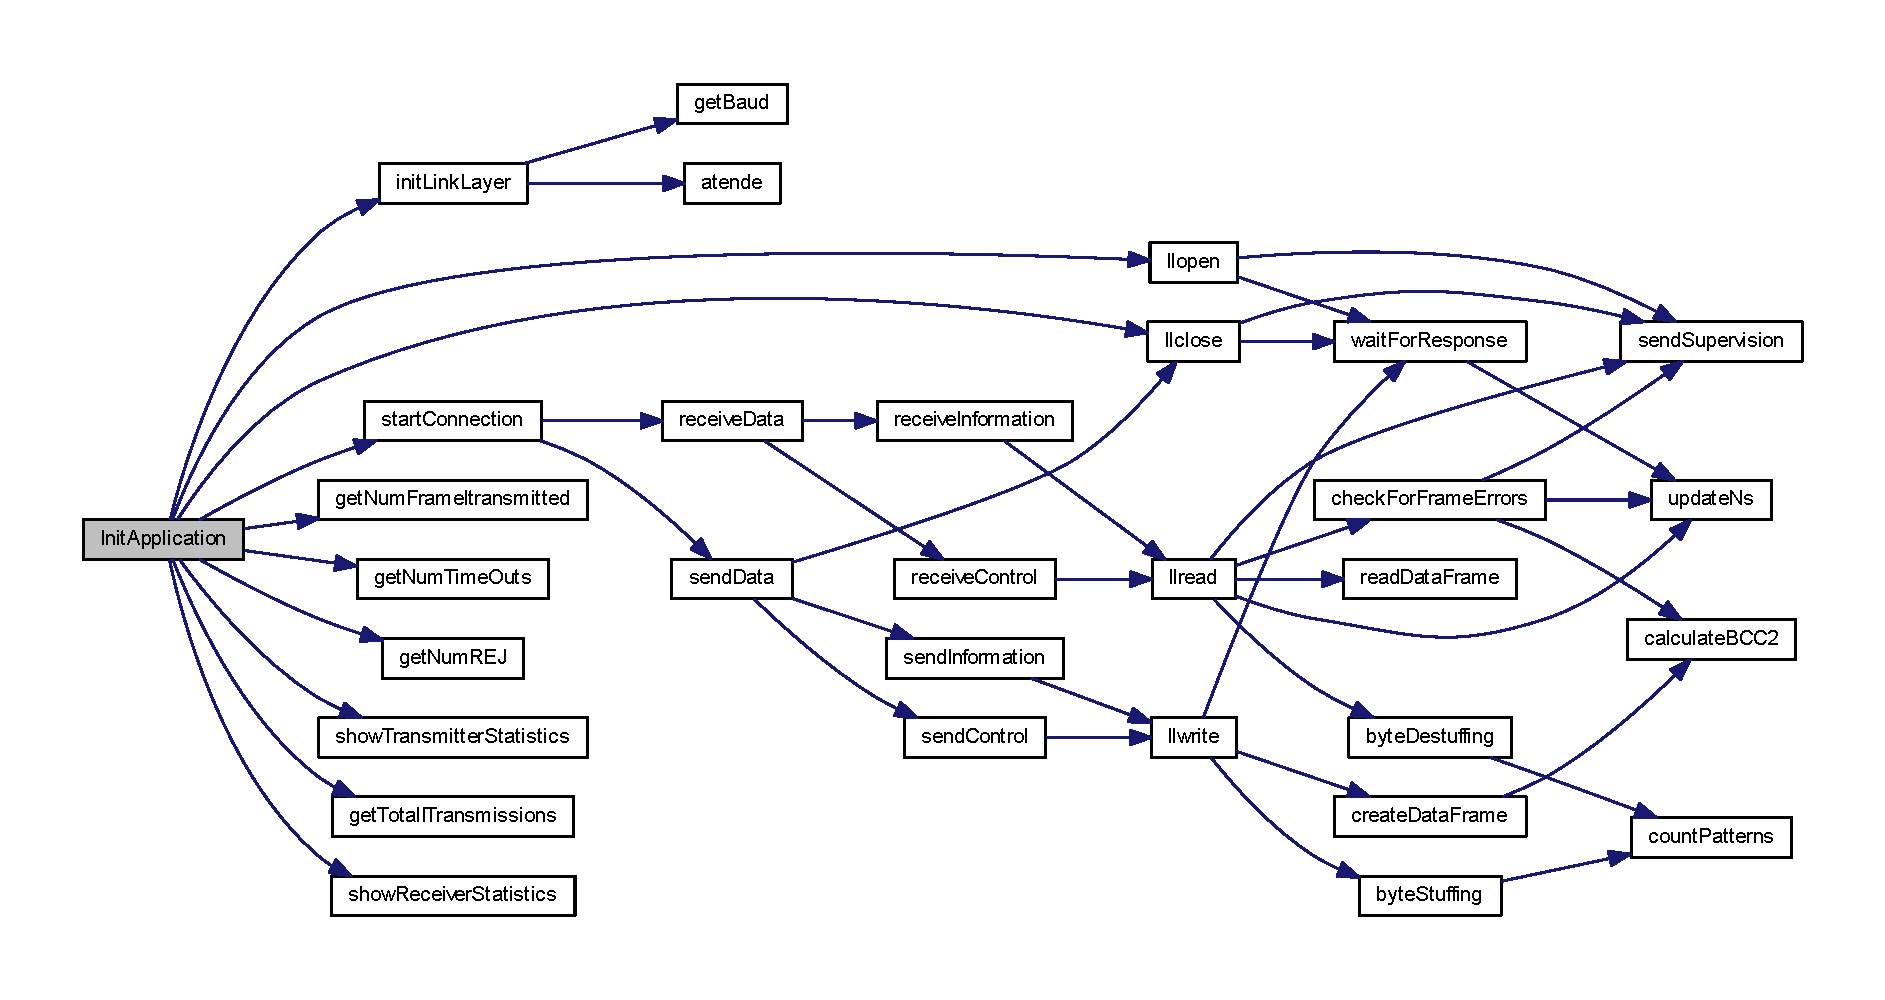
\includegraphics[width=350pt]{application_layer_8h_abdd55a6320cd4fbce91a0583d4ad05f5_cgraph}
\end{center}
\end{figure}
Here is the caller graph for this function\+:\nopagebreak
\begin{figure}[H]
\begin{center}
\leavevmode
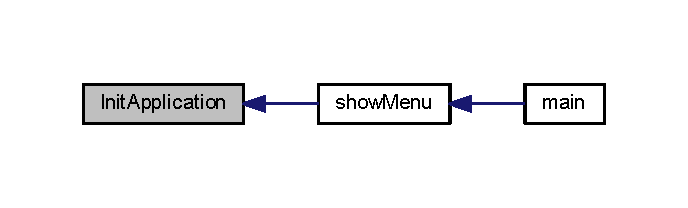
\includegraphics[width=330pt]{application_layer_8h_abdd55a6320cd4fbce91a0583d4ad05f5_icgraph}
\end{center}
\end{figure}
\hypertarget{application_layer_8h_a631126e029a493e74a1af5aacf2a7c16}{}\label{application_layer_8h_a631126e029a493e74a1af5aacf2a7c16} 
\index{application\+Layer.\+h@{application\+Layer.\+h}!receive\+Control@{receive\+Control}}
\index{receive\+Control@{receive\+Control}!application\+Layer.\+h@{application\+Layer.\+h}}
\subsubsection{\texorpdfstring{receive\+Control()}{receiveControl()}}
{\footnotesize\ttfamily int receive\+Control (\begin{DoxyParamCaption}\item[{int}]{type }\end{DoxyParamCaption})}

\mbox{[}receive\+Control description\mbox{]} 
\begin{DoxyParams}{Parameters}
{\em type} & \mbox{[}description\mbox{]} \\
\hline
\end{DoxyParams}
\begin{DoxyReturn}{Returns}
\mbox{[}description\mbox{]} 
\end{DoxyReturn}
Here is the call graph for this function\+:\nopagebreak
\begin{figure}[H]
\begin{center}
\leavevmode
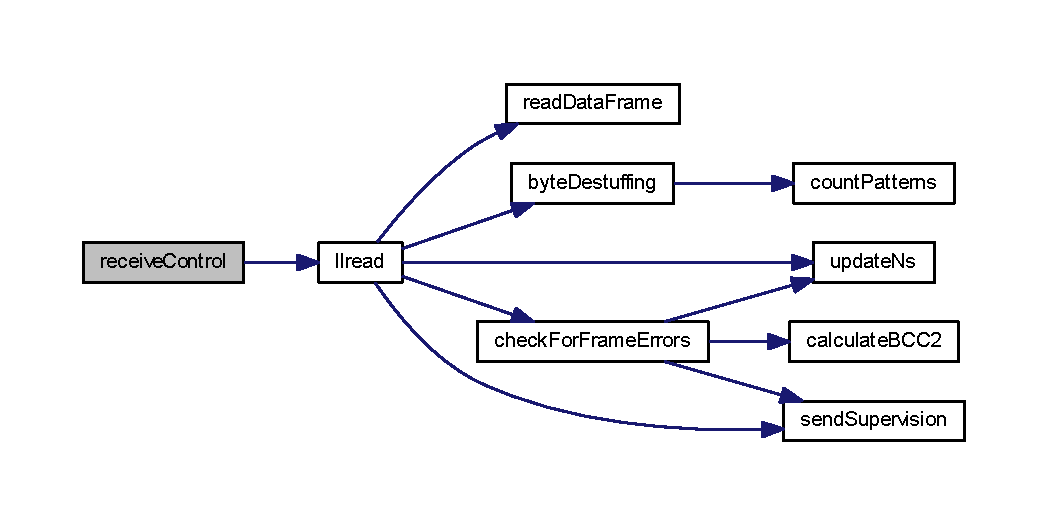
\includegraphics[width=350pt]{application_layer_8h_a631126e029a493e74a1af5aacf2a7c16_cgraph}
\end{center}
\end{figure}
Here is the caller graph for this function\+:\nopagebreak
\begin{figure}[H]
\begin{center}
\leavevmode
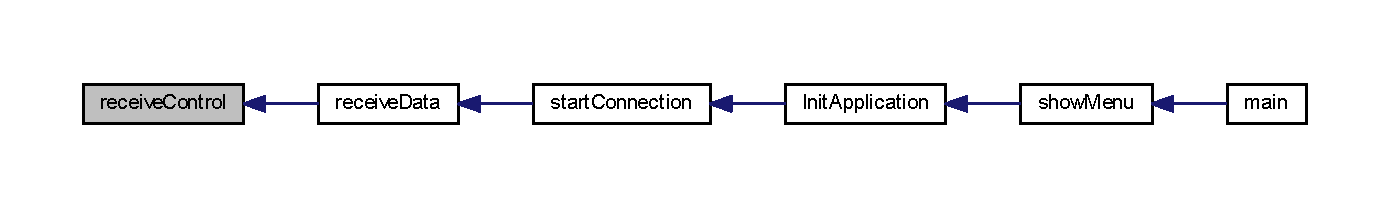
\includegraphics[width=350pt]{application_layer_8h_a631126e029a493e74a1af5aacf2a7c16_icgraph}
\end{center}
\end{figure}
\hypertarget{application_layer_8h_a2809c0419ac7f54685983fd6d3477034}{}\label{application_layer_8h_a2809c0419ac7f54685983fd6d3477034} 
\index{application\+Layer.\+h@{application\+Layer.\+h}!receive\+Data@{receive\+Data}}
\index{receive\+Data@{receive\+Data}!application\+Layer.\+h@{application\+Layer.\+h}}
\subsubsection{\texorpdfstring{receive\+Data()}{receiveData()}}
{\footnotesize\ttfamily int receive\+Data (\begin{DoxyParamCaption}{ }\end{DoxyParamCaption})}

\mbox{[}receive\+Data description\mbox{]} \begin{DoxyReturn}{Returns}
\mbox{[}description\mbox{]} 
\end{DoxyReturn}
Here is the call graph for this function\+:\nopagebreak
\begin{figure}[H]
\begin{center}
\leavevmode
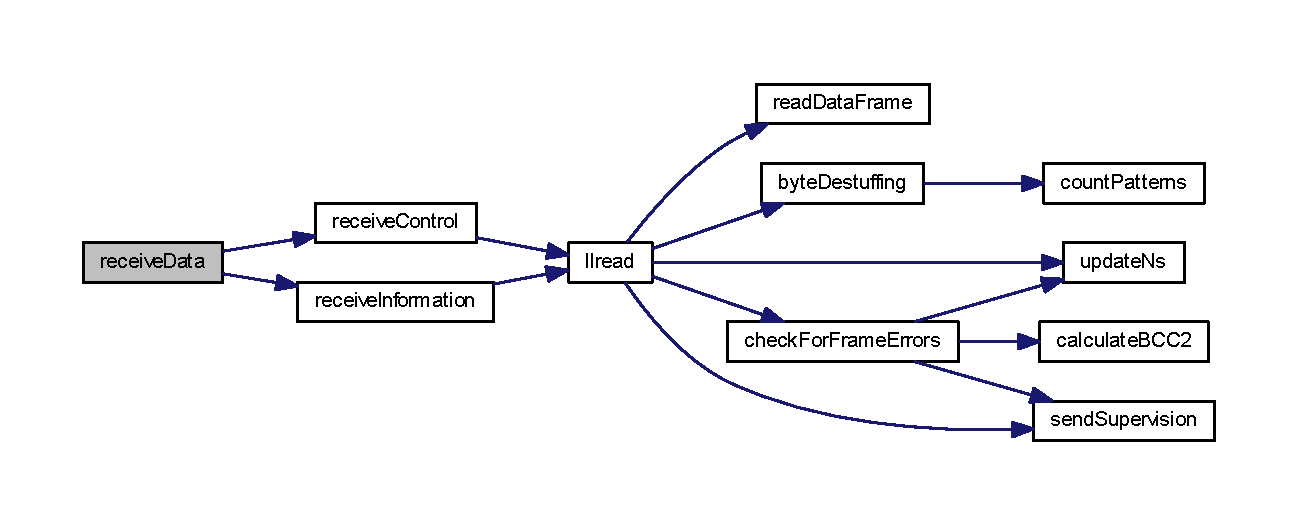
\includegraphics[width=350pt]{application_layer_8h_a2809c0419ac7f54685983fd6d3477034_cgraph}
\end{center}
\end{figure}
Here is the caller graph for this function\+:\nopagebreak
\begin{figure}[H]
\begin{center}
\leavevmode
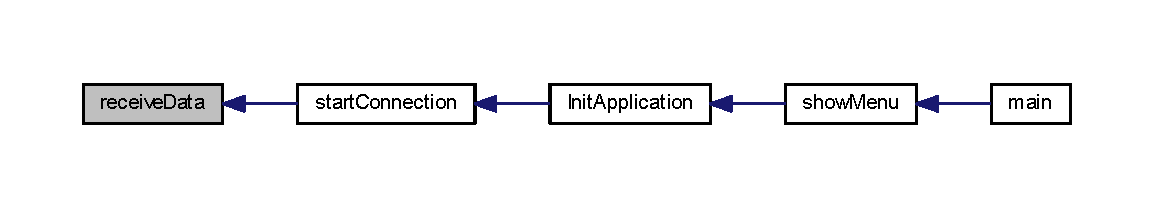
\includegraphics[width=350pt]{application_layer_8h_a2809c0419ac7f54685983fd6d3477034_icgraph}
\end{center}
\end{figure}
\hypertarget{application_layer_8h_a931c3be900b6917c46372f158c19022b}{}\label{application_layer_8h_a931c3be900b6917c46372f158c19022b} 
\index{application\+Layer.\+h@{application\+Layer.\+h}!receive\+Information@{receive\+Information}}
\index{receive\+Information@{receive\+Information}!application\+Layer.\+h@{application\+Layer.\+h}}
\subsubsection{\texorpdfstring{receive\+Information()}{receiveInformation()}}
{\footnotesize\ttfamily int receive\+Information (\begin{DoxyParamCaption}\item[{unsigned char $\ast$}]{buffer,  }\item[{int $\ast$}]{length }\end{DoxyParamCaption})}

\mbox{[}receive\+Information description\mbox{]} 
\begin{DoxyParams}{Parameters}
{\em buffer} & \mbox{[}description\mbox{]} \\
\hline
{\em length} & \mbox{[}description\mbox{]} \\
\hline
\end{DoxyParams}
\begin{DoxyReturn}{Returns}
\mbox{[}description\mbox{]} 
\end{DoxyReturn}
Here is the call graph for this function\+:\nopagebreak
\begin{figure}[H]
\begin{center}
\leavevmode
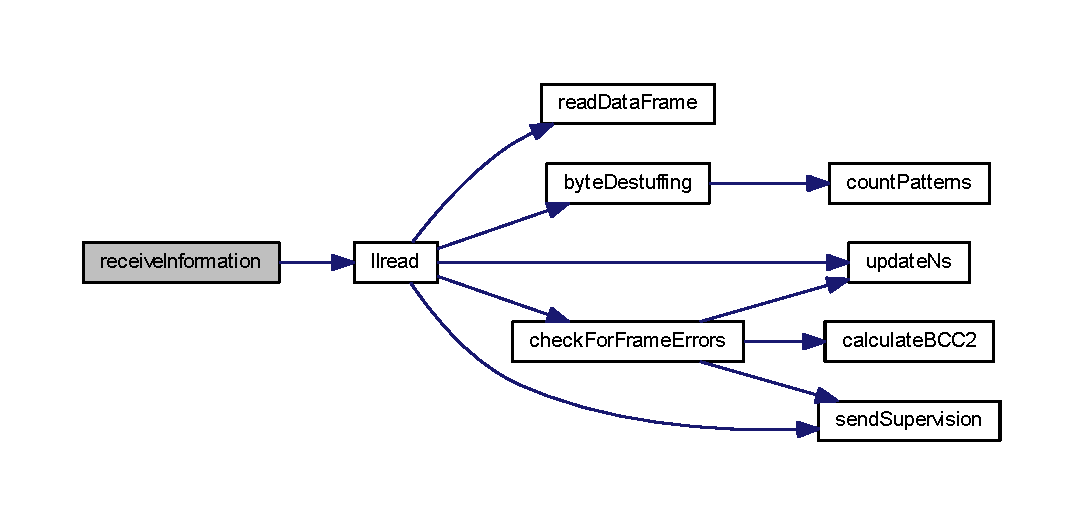
\includegraphics[width=350pt]{application_layer_8h_a931c3be900b6917c46372f158c19022b_cgraph}
\end{center}
\end{figure}
Here is the caller graph for this function\+:\nopagebreak
\begin{figure}[H]
\begin{center}
\leavevmode
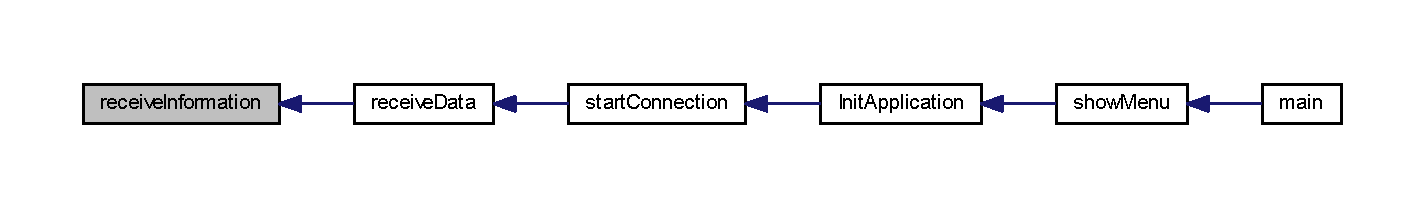
\includegraphics[width=350pt]{application_layer_8h_a931c3be900b6917c46372f158c19022b_icgraph}
\end{center}
\end{figure}
\hypertarget{application_layer_8h_a73ecb47d14db1fb6e2554940364ff040}{}\label{application_layer_8h_a73ecb47d14db1fb6e2554940364ff040} 
\index{application\+Layer.\+h@{application\+Layer.\+h}!send\+Control@{send\+Control}}
\index{send\+Control@{send\+Control}!application\+Layer.\+h@{application\+Layer.\+h}}
\subsubsection{\texorpdfstring{send\+Control()}{sendControl()}}
{\footnotesize\ttfamily int send\+Control (\begin{DoxyParamCaption}\item[{int}]{type }\end{DoxyParamCaption})}

\mbox{[}send\+Control description\mbox{]} 
\begin{DoxyParams}{Parameters}
{\em type} & \mbox{[}description\mbox{]} \\
\hline
\end{DoxyParams}
\begin{DoxyReturn}{Returns}
\mbox{[}description\mbox{]} 
\end{DoxyReturn}
Here is the call graph for this function\+:\nopagebreak
\begin{figure}[H]
\begin{center}
\leavevmode
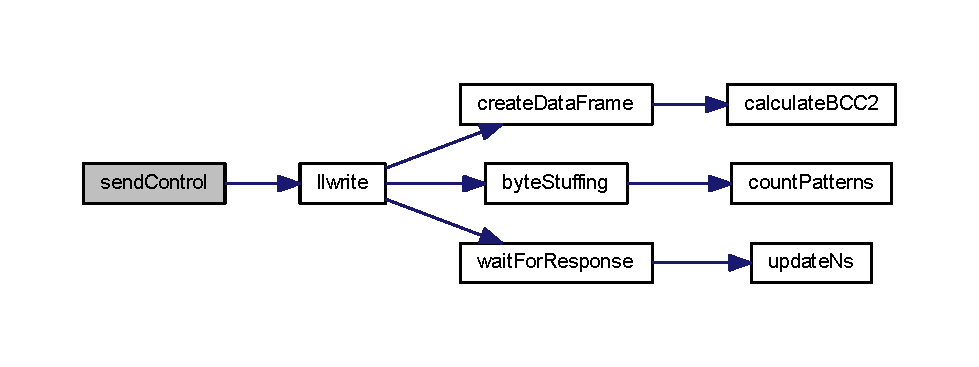
\includegraphics[width=350pt]{application_layer_8h_a73ecb47d14db1fb6e2554940364ff040_cgraph}
\end{center}
\end{figure}
Here is the caller graph for this function\+:\nopagebreak
\begin{figure}[H]
\begin{center}
\leavevmode
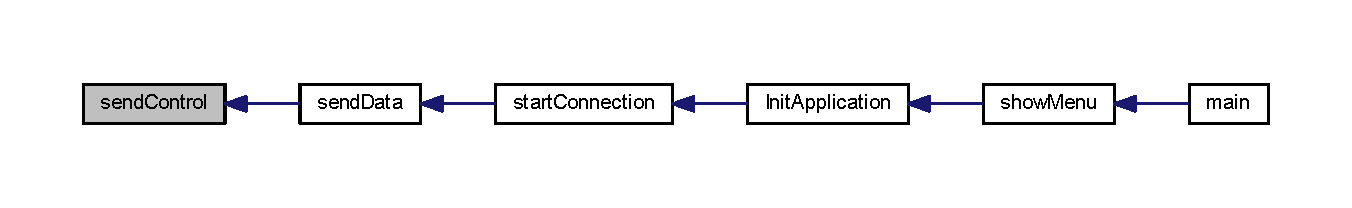
\includegraphics[width=350pt]{application_layer_8h_a73ecb47d14db1fb6e2554940364ff040_icgraph}
\end{center}
\end{figure}
\hypertarget{application_layer_8h_a558000e1f87b3b852f73e20ba0a6b0f4}{}\label{application_layer_8h_a558000e1f87b3b852f73e20ba0a6b0f4} 
\index{application\+Layer.\+h@{application\+Layer.\+h}!send\+Data@{send\+Data}}
\index{send\+Data@{send\+Data}!application\+Layer.\+h@{application\+Layer.\+h}}
\subsubsection{\texorpdfstring{send\+Data()}{sendData()}}
{\footnotesize\ttfamily int send\+Data (\begin{DoxyParamCaption}{ }\end{DoxyParamCaption})}

\mbox{[}send\+Data description\mbox{]} \begin{DoxyReturn}{Returns}
\mbox{[}description\mbox{]} 
\end{DoxyReturn}
Here is the call graph for this function\+:\nopagebreak
\begin{figure}[H]
\begin{center}
\leavevmode
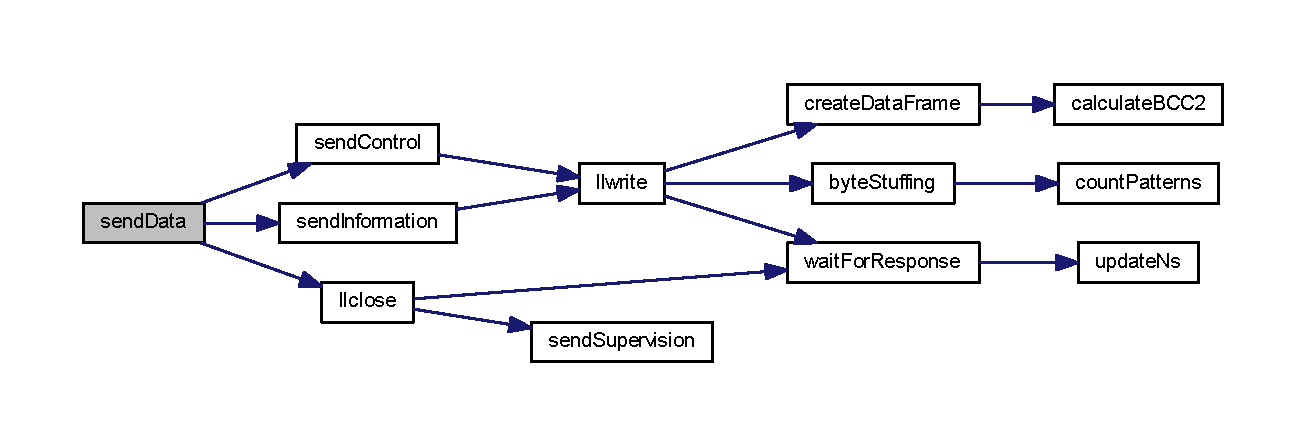
\includegraphics[width=350pt]{application_layer_8h_a558000e1f87b3b852f73e20ba0a6b0f4_cgraph}
\end{center}
\end{figure}
Here is the caller graph for this function\+:\nopagebreak
\begin{figure}[H]
\begin{center}
\leavevmode
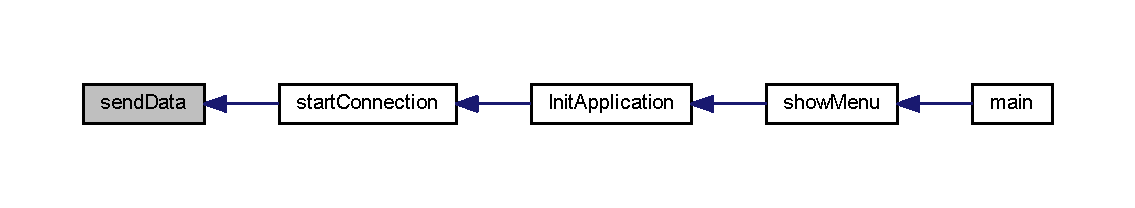
\includegraphics[width=350pt]{application_layer_8h_a558000e1f87b3b852f73e20ba0a6b0f4_icgraph}
\end{center}
\end{figure}
\hypertarget{application_layer_8h_a7a2e353b862e29a450830649a7f113c9}{}\label{application_layer_8h_a7a2e353b862e29a450830649a7f113c9} 
\index{application\+Layer.\+h@{application\+Layer.\+h}!send\+Information@{send\+Information}}
\index{send\+Information@{send\+Information}!application\+Layer.\+h@{application\+Layer.\+h}}
\subsubsection{\texorpdfstring{send\+Information()}{sendInformation()}}
{\footnotesize\ttfamily int send\+Information (\begin{DoxyParamCaption}\item[{unsigned char $\ast$}]{buffer,  }\item[{int}]{length }\end{DoxyParamCaption})}

\mbox{[}send\+Information description\mbox{]} 
\begin{DoxyParams}{Parameters}
{\em buffer} & \mbox{[}description\mbox{]} \\
\hline
{\em length} & \mbox{[}description\mbox{]} \\
\hline
\end{DoxyParams}
\begin{DoxyReturn}{Returns}
\mbox{[}description\mbox{]} 
\end{DoxyReturn}
Here is the call graph for this function\+:\nopagebreak
\begin{figure}[H]
\begin{center}
\leavevmode
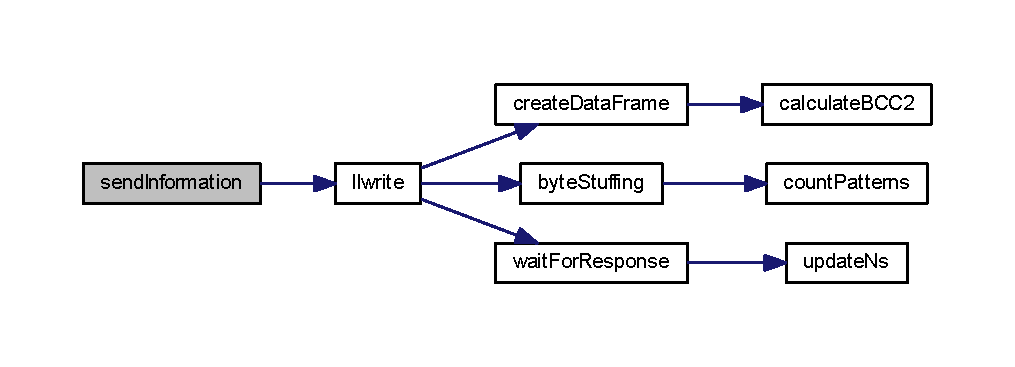
\includegraphics[width=350pt]{application_layer_8h_a7a2e353b862e29a450830649a7f113c9_cgraph}
\end{center}
\end{figure}
Here is the caller graph for this function\+:\nopagebreak
\begin{figure}[H]
\begin{center}
\leavevmode
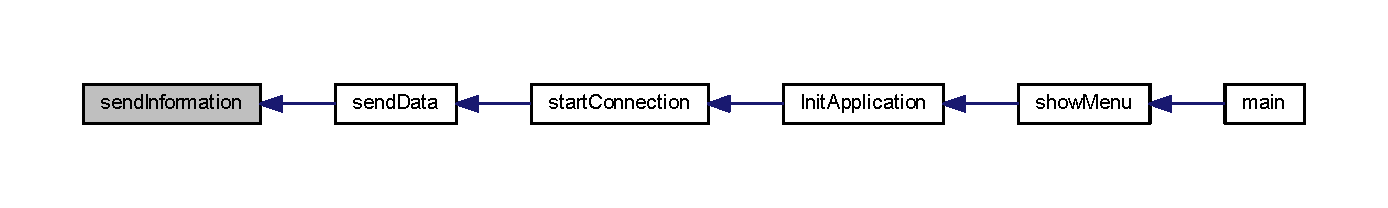
\includegraphics[width=350pt]{application_layer_8h_a7a2e353b862e29a450830649a7f113c9_icgraph}
\end{center}
\end{figure}
\hypertarget{application_layer_8h_a0ac5863989f90535cb0fecae68437202}{}\label{application_layer_8h_a0ac5863989f90535cb0fecae68437202} 
\index{application\+Layer.\+h@{application\+Layer.\+h}!show\+Receiver\+Statistics@{show\+Receiver\+Statistics}}
\index{show\+Receiver\+Statistics@{show\+Receiver\+Statistics}!application\+Layer.\+h@{application\+Layer.\+h}}
\subsubsection{\texorpdfstring{show\+Receiver\+Statistics()}{showReceiverStatistics()}}
{\footnotesize\ttfamily int show\+Receiver\+Statistics (\begin{DoxyParamCaption}\item[{int}]{num\+R\+E\+Jtransmissions,  }\item[{int}]{num\+Total\+I\+Transmissions }\end{DoxyParamCaption})}

Here is the caller graph for this function\+:\nopagebreak
\begin{figure}[H]
\begin{center}
\leavevmode
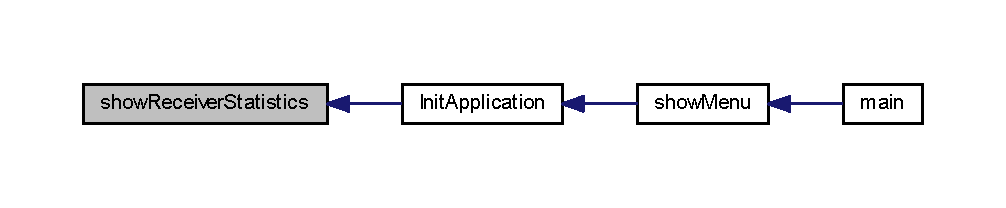
\includegraphics[width=350pt]{application_layer_8h_a0ac5863989f90535cb0fecae68437202_icgraph}
\end{center}
\end{figure}
\hypertarget{application_layer_8h_ab2509db0c3dc8c88c9a678df0120bc21}{}\label{application_layer_8h_ab2509db0c3dc8c88c9a678df0120bc21} 
\index{application\+Layer.\+h@{application\+Layer.\+h}!show\+Transmitter\+Statistics@{show\+Transmitter\+Statistics}}
\index{show\+Transmitter\+Statistics@{show\+Transmitter\+Statistics}!application\+Layer.\+h@{application\+Layer.\+h}}
\subsubsection{\texorpdfstring{show\+Transmitter\+Statistics()}{showTransmitterStatistics()}}
{\footnotesize\ttfamily int show\+Transmitter\+Statistics (\begin{DoxyParamCaption}\item[{int}]{num\+R\+E\+Jreceived,  }\item[{int}]{num\+Frame\+Itransmitted,  }\item[{int}]{num\+Time\+Outs }\end{DoxyParamCaption})}

Here is the caller graph for this function\+:\nopagebreak
\begin{figure}[H]
\begin{center}
\leavevmode
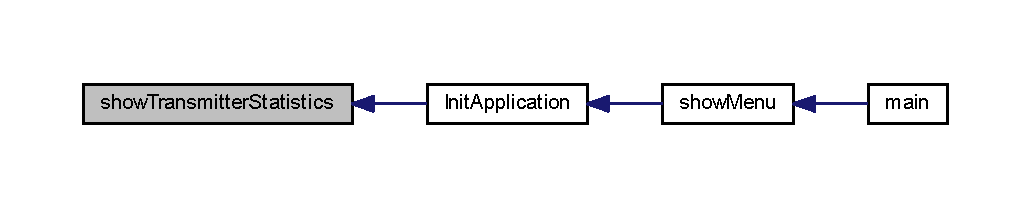
\includegraphics[width=350pt]{application_layer_8h_ab2509db0c3dc8c88c9a678df0120bc21_icgraph}
\end{center}
\end{figure}
\hypertarget{application_layer_8h_a3622090a7ff391221a74cad6493bbca9}{}\label{application_layer_8h_a3622090a7ff391221a74cad6493bbca9} 
\index{application\+Layer.\+h@{application\+Layer.\+h}!start\+Connection@{start\+Connection}}
\index{start\+Connection@{start\+Connection}!application\+Layer.\+h@{application\+Layer.\+h}}
\subsubsection{\texorpdfstring{start\+Connection()}{startConnection()}}
{\footnotesize\ttfamily int start\+Connection (\begin{DoxyParamCaption}{ }\end{DoxyParamCaption})}

\mbox{[}start\+Connection description\mbox{]} \begin{DoxyReturn}{Returns}
\mbox{[}description\mbox{]} 
\end{DoxyReturn}
Here is the call graph for this function\+:\nopagebreak
\begin{figure}[H]
\begin{center}
\leavevmode
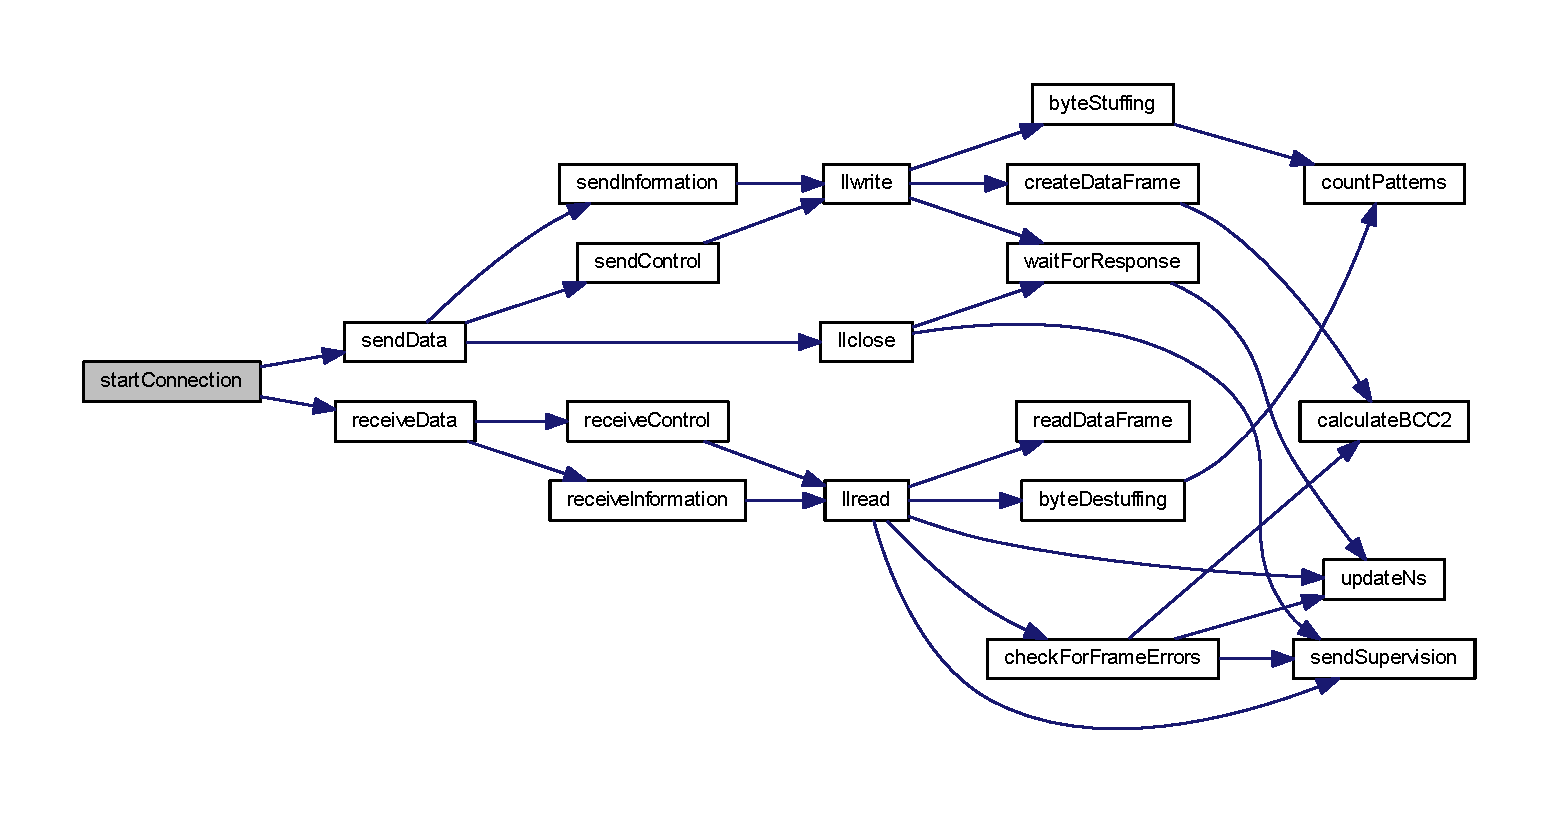
\includegraphics[width=350pt]{application_layer_8h_a3622090a7ff391221a74cad6493bbca9_cgraph}
\end{center}
\end{figure}
Here is the caller graph for this function\+:\nopagebreak
\begin{figure}[H]
\begin{center}
\leavevmode
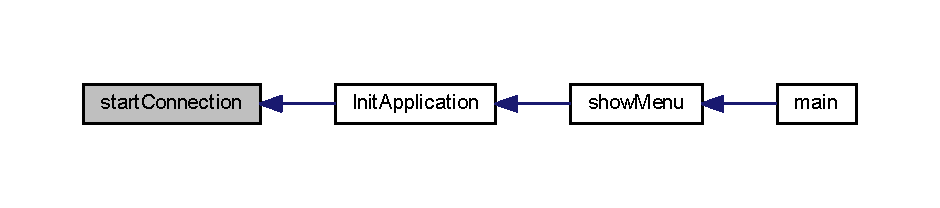
\includegraphics[width=350pt]{application_layer_8h_a3622090a7ff391221a74cad6493bbca9_icgraph}
\end{center}
\end{figure}

\hypertarget{link_layer_8c}{}\section{link\+Layer.\+c File Reference}
\label{link_layer_8c}\index{link\+Layer.\+c@{link\+Layer.\+c}}
{\ttfamily \#include \char`\"{}link\+Layer.\+h\char`\"{}}\newline
Include dependency graph for link\+Layer.\+c\+:\nopagebreak
\begin{figure}[H]
\begin{center}
\leavevmode
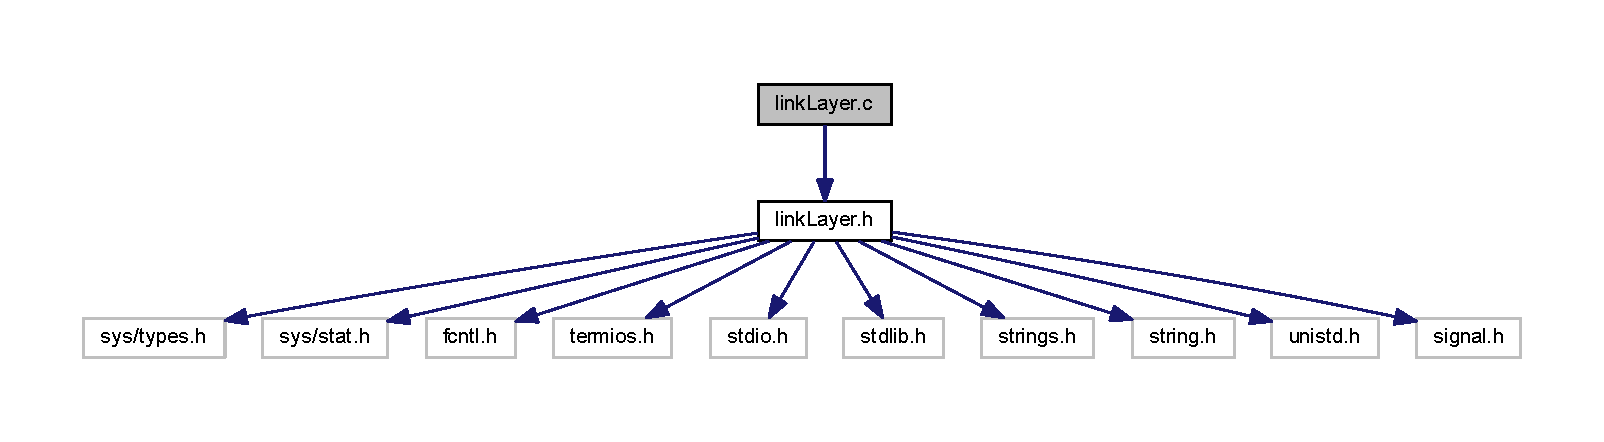
\includegraphics[width=350pt]{link_layer_8c__incl}
\end{center}
\end{figure}
\subsection*{Enumerations}
\begin{DoxyCompactItemize}
\item 
enum \hyperlink{link_layer_8c_adc6e5733fc3c22f0a7b2914188c49c90}{state} \{ \newline
\hyperlink{link_layer_8c_adc6e5733fc3c22f0a7b2914188c49c90a0e97c69c73117f6c0109b2d7d1d9cedc}{start}, 
\hyperlink{link_layer_8c_adc6e5733fc3c22f0a7b2914188c49c90a30f2e168fe65f5a7d61615be13b59214}{flag\+R\+CV}, 
\hyperlink{link_layer_8c_adc6e5733fc3c22f0a7b2914188c49c90a46e22e708475b4203cedbdcd334f563d}{a\+R\+CV}, 
\hyperlink{link_layer_8c_adc6e5733fc3c22f0a7b2914188c49c90af250a70af62fb1789123574dfa5637a6}{c\+R\+CV}, 
\newline
\hyperlink{link_layer_8c_adc6e5733fc3c22f0a7b2914188c49c90a90184d1ca3f40e4499024f6df6ddab2f}{B\+CC}, 
\hyperlink{link_layer_8c_adc6e5733fc3c22f0a7b2914188c49c90ad82a4ca4dc1f04bf9453ad19f9341028}{stop}
 \}
\end{DoxyCompactItemize}
\subsection*{Functions}
\begin{DoxyCompactItemize}
\item 
int \hyperlink{link_layer_8c_a911024c5b110489238e2e29e119c93b0}{init\+Link\+Layer} (int port, int status, int baudrate, int \hyperlink{main_8c_a8ba735ab56b2afeb844916994c86f3f5}{retries}, int timeout)
\item 
int \hyperlink{link_layer_8c_a3d8522ab922e18bc1571ae49767b55e9}{llopen} (int fd)
\item 
int \hyperlink{link_layer_8c_a343e4b5928516727236a390a25f28c77}{llclose} (int fd)
\item 
int \hyperlink{link_layer_8c_a363d12e859b97c186f6b28c96934bad4}{llwrite} (unsigned char $\ast$buffer, int length, int fd)
\item 
int \hyperlink{link_layer_8c_a520783778c9b115983967fe315306e36}{check\+For\+Frame\+Errors} (int fd, unsigned char $\ast$buffer, unsigned char $\ast$package, int length, int data\+Size)
\item 
int \hyperlink{link_layer_8c_a8a2fe283b8290cc1336a667a712cc187}{llread} (int fd, unsigned char $\ast$package, int num\+Frame)
\item 
int \hyperlink{link_layer_8c_af4c7f81a4d22d375976891988ef065c8}{send\+Supervision} (int fd, unsigned char control)
\item 
unsigned char \hyperlink{link_layer_8c_aaa527233d90b0499478a918eea3f1d19}{calculate\+B\+C\+C2} (unsigned char $\ast$frame, int length)
\item 
unsigned char $\ast$ \hyperlink{link_layer_8c_ac32e18813599af0fd5db007dbc943bd9}{create\+Data\+Frame} (unsigned char $\ast$buffer, int length)
\item 
int \hyperlink{link_layer_8c_a3a87048128ef21ca08862bf197517143}{wait\+For\+Response} (int fd, unsigned char flag\+Type)
\item 
int \hyperlink{link_layer_8c_aa6727c503e5fa4edab84052556382a11}{count\+Patterns} (unsigned char $\ast$$\ast$frame, int length)
\item 
int \hyperlink{link_layer_8c_a1295fa2e6765acc35b05d8cb9dc9e9a1}{byte\+Stuffing} (unsigned char $\ast$$\ast$frame, int length)
\item 
int \hyperlink{link_layer_8c_a888914efd19822deb27e1f0a5cacca94}{byte\+Destuffing} (unsigned char $\ast$$\ast$frame, int length)
\item 
void \hyperlink{link_layer_8c_adc4d249c47efd1729a17f2782de863c2}{atende} ()
\item 
int \hyperlink{link_layer_8c_abfbd40d058faa134b9034af9d2d865d9}{read\+Data\+Frame} (int fd, unsigned char $\ast$frame)
\item 
void \hyperlink{link_layer_8c_a927fcc5a512622e7fc4b688966241284}{update\+Ns} ()
\item 
int \hyperlink{link_layer_8c_a85cabdbf707b2b7ac21c233044d13f0e}{get\+Baud} (int baudrate)
\item 
int \hyperlink{link_layer_8c_a1d6d156ac0b76c0b763bd86644697c0c}{get\+Num\+R\+EJ} ()
\item 
int \hyperlink{link_layer_8c_affeeaaec470b74e3d98431a3841ffc4f}{get\+Total\+I\+Transmissions} ()
\item 
int \hyperlink{link_layer_8c_a7ff6916ccba0812bd39d4f06eb25af2c}{get\+Num\+Frame\+Itransmitted} ()
\item 
int \hyperlink{link_layer_8c_acf7f29601204c0a58a804bcadd2e46c9}{get\+Num\+Time\+Outs} ()
\end{DoxyCompactItemize}
\subsection*{Variables}
\begin{DoxyCompactItemize}
\item 
volatile int \hyperlink{link_layer_8c_a5fbc721140a2ca81a3fcbdafaa668bdd}{S\+T\+OP} =\hyperlink{link_layer_8h_aa93f0eb578d23995850d61f7d61c55c1}{F\+A\+L\+SE}
\item 
int \hyperlink{link_layer_8c_ae2c6087027bfdf561a2b766975b47ee8}{timer} = 1
\item 
int \hyperlink{link_layer_8c_adf916204820072417ed73a32de1cefcf}{flag} = 1
\item 
\hyperlink{struct_link_layer}{Link\+Layer} $\ast$ \hyperlink{link_layer_8c_a70df012765479ea774aa425d7527e718}{link\+Layer}
\item 
int \hyperlink{link_layer_8c_a149b5ea0e56df54ba2f74166453a8fd9}{num\+FrameI} = 0
\item 
int \hyperlink{link_layer_8c_a0637f6d853eaa5a7e5bead66bc9ee567}{num\+Frame\+Itransmitted} = 0
\item 
int \hyperlink{link_layer_8c_ad28672c114a1578ed97b0a73abbdc761}{num\+Time\+Outs} = 0
\item 
int \hyperlink{link_layer_8c_a08882678e9b70455b991496b0bf0f55b}{num\+R\+E\+Jreceived} = 0
\end{DoxyCompactItemize}


\subsection{Enumeration Type Documentation}
\hypertarget{link_layer_8c_adc6e5733fc3c22f0a7b2914188c49c90}{}\label{link_layer_8c_adc6e5733fc3c22f0a7b2914188c49c90} 
\index{link\+Layer.\+c@{link\+Layer.\+c}!state@{state}}
\index{state@{state}!link\+Layer.\+c@{link\+Layer.\+c}}
\subsubsection{\texorpdfstring{state}{state}}
{\footnotesize\ttfamily enum \hyperlink{link_layer_8c_adc6e5733fc3c22f0a7b2914188c49c90}{state}}

\begin{DoxyEnumFields}{Enumerator}
\raisebox{\heightof{T}}[0pt][0pt]{\index{start@{start}!link\+Layer.\+c@{link\+Layer.\+c}}\index{link\+Layer.\+c@{link\+Layer.\+c}!start@{start}}}\hypertarget{link_layer_8c_adc6e5733fc3c22f0a7b2914188c49c90a0e97c69c73117f6c0109b2d7d1d9cedc}{}\label{link_layer_8c_adc6e5733fc3c22f0a7b2914188c49c90a0e97c69c73117f6c0109b2d7d1d9cedc} 
start&\\
\hline

\raisebox{\heightof{T}}[0pt][0pt]{\index{flag\+R\+CV@{flag\+R\+CV}!link\+Layer.\+c@{link\+Layer.\+c}}\index{link\+Layer.\+c@{link\+Layer.\+c}!flag\+R\+CV@{flag\+R\+CV}}}\hypertarget{link_layer_8c_adc6e5733fc3c22f0a7b2914188c49c90a30f2e168fe65f5a7d61615be13b59214}{}\label{link_layer_8c_adc6e5733fc3c22f0a7b2914188c49c90a30f2e168fe65f5a7d61615be13b59214} 
flag\+R\+CV&\\
\hline

\raisebox{\heightof{T}}[0pt][0pt]{\index{a\+R\+CV@{a\+R\+CV}!link\+Layer.\+c@{link\+Layer.\+c}}\index{link\+Layer.\+c@{link\+Layer.\+c}!a\+R\+CV@{a\+R\+CV}}}\hypertarget{link_layer_8c_adc6e5733fc3c22f0a7b2914188c49c90a46e22e708475b4203cedbdcd334f563d}{}\label{link_layer_8c_adc6e5733fc3c22f0a7b2914188c49c90a46e22e708475b4203cedbdcd334f563d} 
a\+R\+CV&\\
\hline

\raisebox{\heightof{T}}[0pt][0pt]{\index{c\+R\+CV@{c\+R\+CV}!link\+Layer.\+c@{link\+Layer.\+c}}\index{link\+Layer.\+c@{link\+Layer.\+c}!c\+R\+CV@{c\+R\+CV}}}\hypertarget{link_layer_8c_adc6e5733fc3c22f0a7b2914188c49c90af250a70af62fb1789123574dfa5637a6}{}\label{link_layer_8c_adc6e5733fc3c22f0a7b2914188c49c90af250a70af62fb1789123574dfa5637a6} 
c\+R\+CV&\\
\hline

\raisebox{\heightof{T}}[0pt][0pt]{\index{B\+CC@{B\+CC}!link\+Layer.\+c@{link\+Layer.\+c}}\index{link\+Layer.\+c@{link\+Layer.\+c}!B\+CC@{B\+CC}}}\hypertarget{link_layer_8c_adc6e5733fc3c22f0a7b2914188c49c90a90184d1ca3f40e4499024f6df6ddab2f}{}\label{link_layer_8c_adc6e5733fc3c22f0a7b2914188c49c90a90184d1ca3f40e4499024f6df6ddab2f} 
B\+CC&\\
\hline

\raisebox{\heightof{T}}[0pt][0pt]{\index{stop@{stop}!link\+Layer.\+c@{link\+Layer.\+c}}\index{link\+Layer.\+c@{link\+Layer.\+c}!stop@{stop}}}\hypertarget{link_layer_8c_adc6e5733fc3c22f0a7b2914188c49c90ad82a4ca4dc1f04bf9453ad19f9341028}{}\label{link_layer_8c_adc6e5733fc3c22f0a7b2914188c49c90ad82a4ca4dc1f04bf9453ad19f9341028} 
stop&\\
\hline

\end{DoxyEnumFields}


\subsection{Function Documentation}
\hypertarget{link_layer_8c_adc4d249c47efd1729a17f2782de863c2}{}\label{link_layer_8c_adc4d249c47efd1729a17f2782de863c2} 
\index{link\+Layer.\+c@{link\+Layer.\+c}!atende@{atende}}
\index{atende@{atende}!link\+Layer.\+c@{link\+Layer.\+c}}
\subsubsection{\texorpdfstring{atende()}{atende()}}
{\footnotesize\ttfamily void atende (\begin{DoxyParamCaption}{ }\end{DoxyParamCaption})}

Here is the caller graph for this function\+:
\nopagebreak
\begin{figure}[H]
\begin{center}
\leavevmode
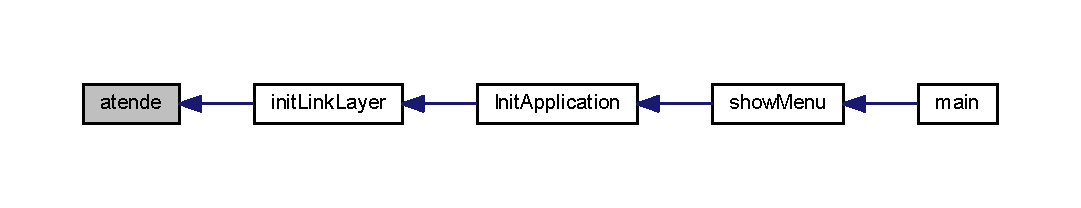
\includegraphics[width=350pt]{link_layer_8c_adc4d249c47efd1729a17f2782de863c2_icgraph}
\end{center}
\end{figure}
\hypertarget{link_layer_8c_a888914efd19822deb27e1f0a5cacca94}{}\label{link_layer_8c_a888914efd19822deb27e1f0a5cacca94} 
\index{link\+Layer.\+c@{link\+Layer.\+c}!byte\+Destuffing@{byte\+Destuffing}}
\index{byte\+Destuffing@{byte\+Destuffing}!link\+Layer.\+c@{link\+Layer.\+c}}
\subsubsection{\texorpdfstring{byte\+Destuffing()}{byteDestuffing()}}
{\footnotesize\ttfamily int byte\+Destuffing (\begin{DoxyParamCaption}\item[{unsigned char $\ast$$\ast$}]{frame,  }\item[{int}]{length }\end{DoxyParamCaption})}


\begin{DoxyParams}{Parameters}
{\em } & \\
\hline
\end{DoxyParams}
Here is the call graph for this function\+:
\nopagebreak
\begin{figure}[H]
\begin{center}
\leavevmode
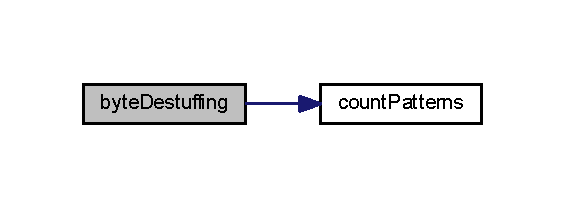
\includegraphics[width=271pt]{link_layer_8c_a888914efd19822deb27e1f0a5cacca94_cgraph}
\end{center}
\end{figure}
Here is the caller graph for this function\+:
\nopagebreak
\begin{figure}[H]
\begin{center}
\leavevmode
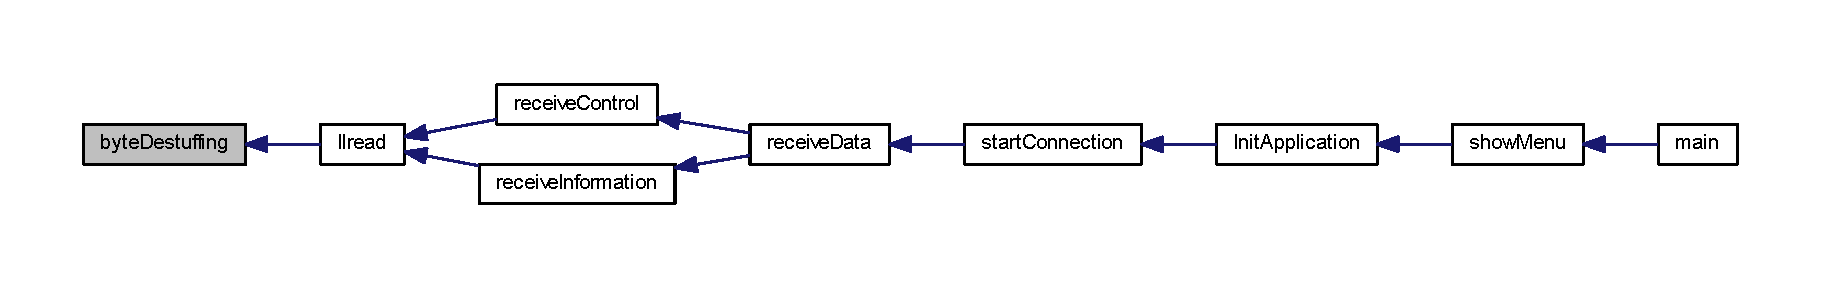
\includegraphics[width=350pt]{link_layer_8c_a888914efd19822deb27e1f0a5cacca94_icgraph}
\end{center}
\end{figure}
\hypertarget{link_layer_8c_a1295fa2e6765acc35b05d8cb9dc9e9a1}{}\label{link_layer_8c_a1295fa2e6765acc35b05d8cb9dc9e9a1} 
\index{link\+Layer.\+c@{link\+Layer.\+c}!byte\+Stuffing@{byte\+Stuffing}}
\index{byte\+Stuffing@{byte\+Stuffing}!link\+Layer.\+c@{link\+Layer.\+c}}
\subsubsection{\texorpdfstring{byte\+Stuffing()}{byteStuffing()}}
{\footnotesize\ttfamily int byte\+Stuffing (\begin{DoxyParamCaption}\item[{unsigned char $\ast$$\ast$}]{frame,  }\item[{int}]{length }\end{DoxyParamCaption})}


\begin{DoxyParams}{Parameters}
{\em } & \\
\hline
\end{DoxyParams}
Here is the call graph for this function\+:
\nopagebreak
\begin{figure}[H]
\begin{center}
\leavevmode
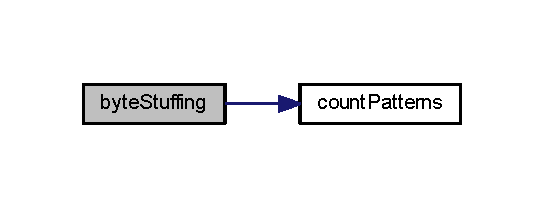
\includegraphics[width=261pt]{link_layer_8c_a1295fa2e6765acc35b05d8cb9dc9e9a1_cgraph}
\end{center}
\end{figure}
Here is the caller graph for this function\+:
\nopagebreak
\begin{figure}[H]
\begin{center}
\leavevmode
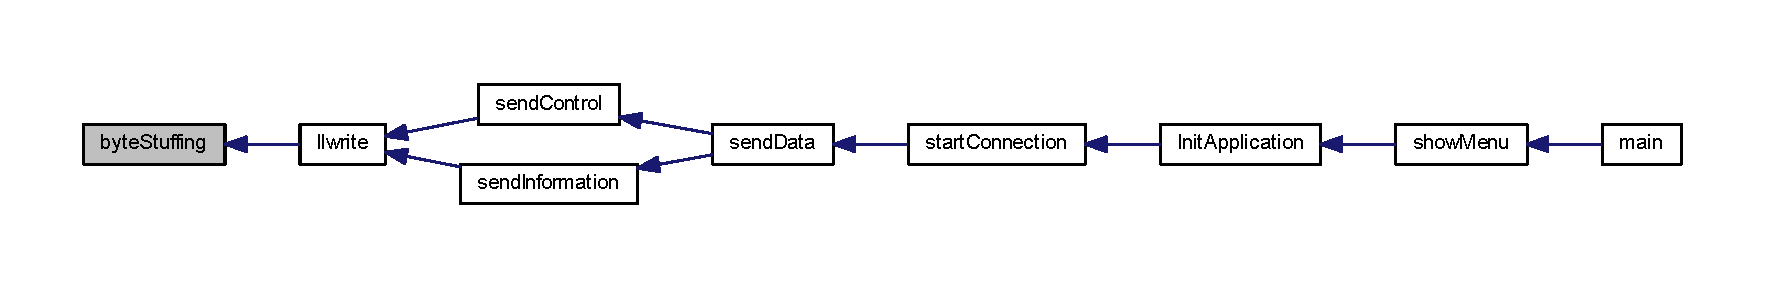
\includegraphics[width=350pt]{link_layer_8c_a1295fa2e6765acc35b05d8cb9dc9e9a1_icgraph}
\end{center}
\end{figure}
\hypertarget{link_layer_8c_aaa527233d90b0499478a918eea3f1d19}{}\label{link_layer_8c_aaa527233d90b0499478a918eea3f1d19} 
\index{link\+Layer.\+c@{link\+Layer.\+c}!calculate\+B\+C\+C2@{calculate\+B\+C\+C2}}
\index{calculate\+B\+C\+C2@{calculate\+B\+C\+C2}!link\+Layer.\+c@{link\+Layer.\+c}}
\subsubsection{\texorpdfstring{calculate\+B\+C\+C2()}{calculateBCC2()}}
{\footnotesize\ttfamily unsigned char calculate\+B\+C\+C2 (\begin{DoxyParamCaption}\item[{unsigned char $\ast$}]{frame,  }\item[{int}]{length }\end{DoxyParamCaption})}

Calculates the X\+OR of the data bytes 
\begin{DoxyParams}{Parameters}
{\em } & \\
\hline
\end{DoxyParams}
Here is the caller graph for this function\+:
\nopagebreak
\begin{figure}[H]
\begin{center}
\leavevmode
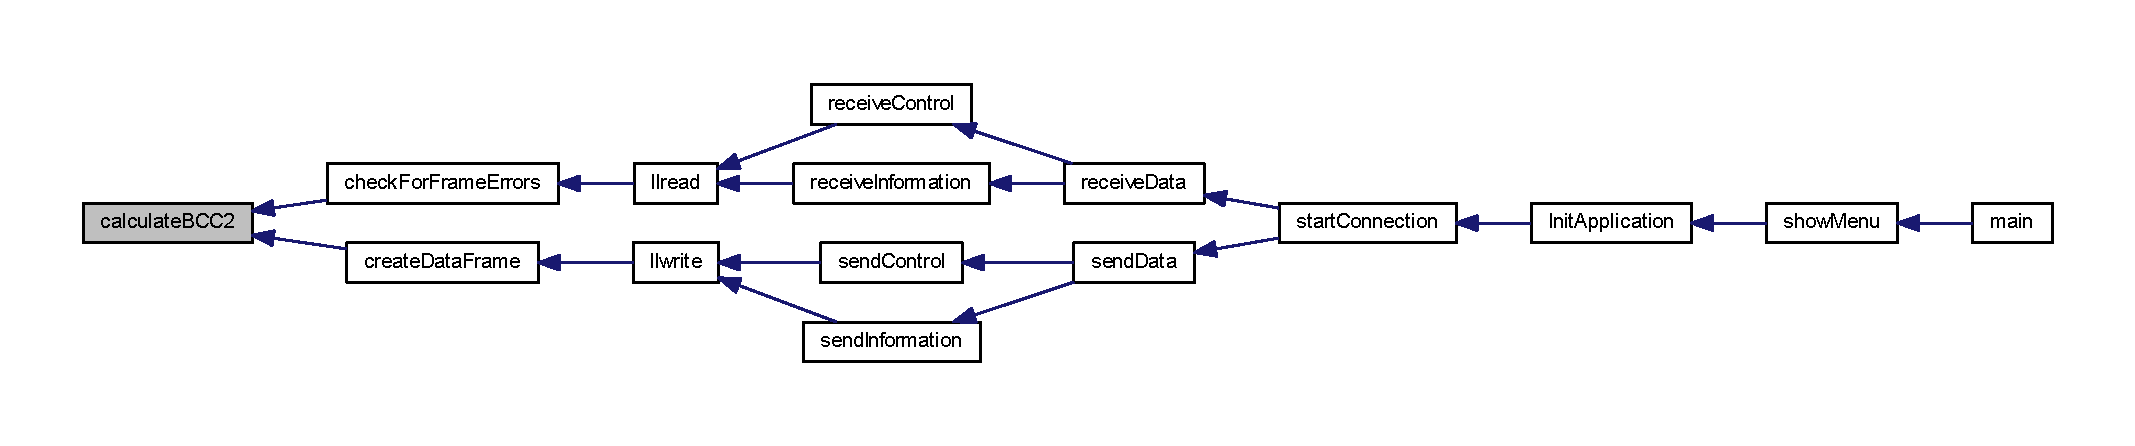
\includegraphics[width=350pt]{link_layer_8c_aaa527233d90b0499478a918eea3f1d19_icgraph}
\end{center}
\end{figure}
\hypertarget{link_layer_8c_a520783778c9b115983967fe315306e36}{}\label{link_layer_8c_a520783778c9b115983967fe315306e36} 
\index{link\+Layer.\+c@{link\+Layer.\+c}!check\+For\+Frame\+Errors@{check\+For\+Frame\+Errors}}
\index{check\+For\+Frame\+Errors@{check\+For\+Frame\+Errors}!link\+Layer.\+c@{link\+Layer.\+c}}
\subsubsection{\texorpdfstring{check\+For\+Frame\+Errors()}{checkForFrameErrors()}}
{\footnotesize\ttfamily int check\+For\+Frame\+Errors (\begin{DoxyParamCaption}\item[{int}]{fd,  }\item[{unsigned char $\ast$}]{buffer,  }\item[{unsigned char $\ast$}]{package,  }\item[{int}]{length,  }\item[{int}]{data\+Size }\end{DoxyParamCaption})}

Here is the call graph for this function\+:
\nopagebreak
\begin{figure}[H]
\begin{center}
\leavevmode
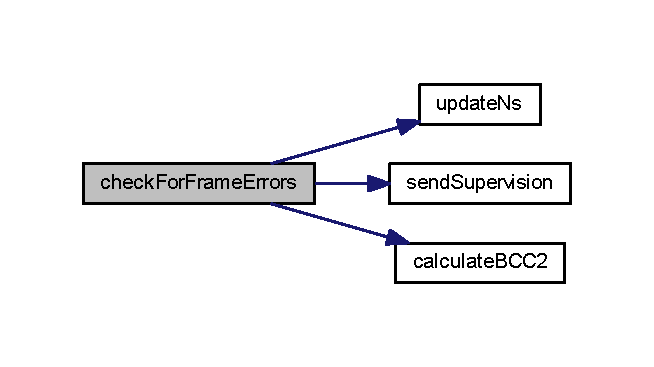
\includegraphics[width=314pt]{link_layer_8c_a520783778c9b115983967fe315306e36_cgraph}
\end{center}
\end{figure}
Here is the caller graph for this function\+:
\nopagebreak
\begin{figure}[H]
\begin{center}
\leavevmode
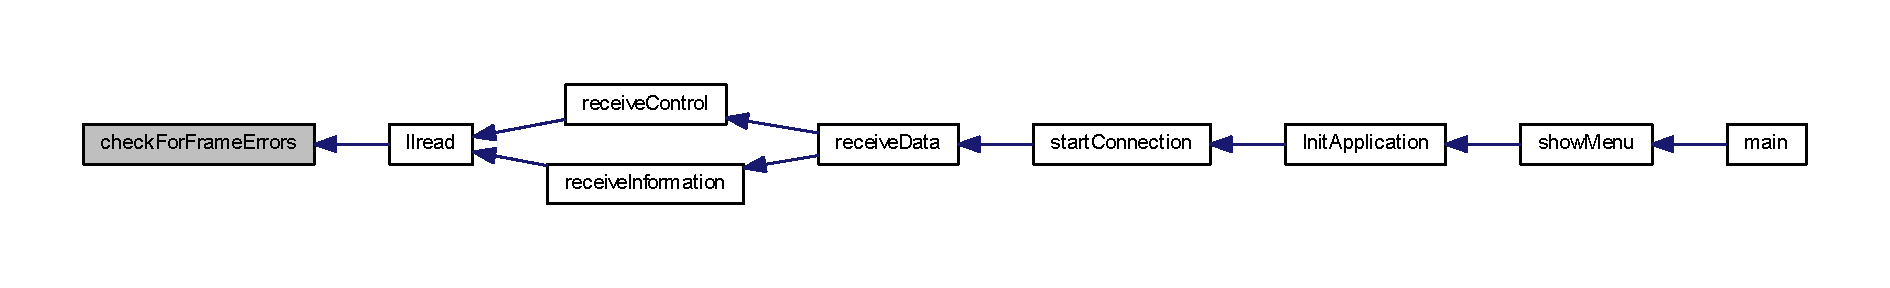
\includegraphics[width=350pt]{link_layer_8c_a520783778c9b115983967fe315306e36_icgraph}
\end{center}
\end{figure}
\hypertarget{link_layer_8c_aa6727c503e5fa4edab84052556382a11}{}\label{link_layer_8c_aa6727c503e5fa4edab84052556382a11} 
\index{link\+Layer.\+c@{link\+Layer.\+c}!count\+Patterns@{count\+Patterns}}
\index{count\+Patterns@{count\+Patterns}!link\+Layer.\+c@{link\+Layer.\+c}}
\subsubsection{\texorpdfstring{count\+Patterns()}{countPatterns()}}
{\footnotesize\ttfamily int count\+Patterns (\begin{DoxyParamCaption}\item[{unsigned char $\ast$$\ast$}]{frame,  }\item[{int}]{length }\end{DoxyParamCaption})}


\begin{DoxyParams}{Parameters}
{\em } & \\
\hline
\end{DoxyParams}
Here is the caller graph for this function\+:
\nopagebreak
\begin{figure}[H]
\begin{center}
\leavevmode
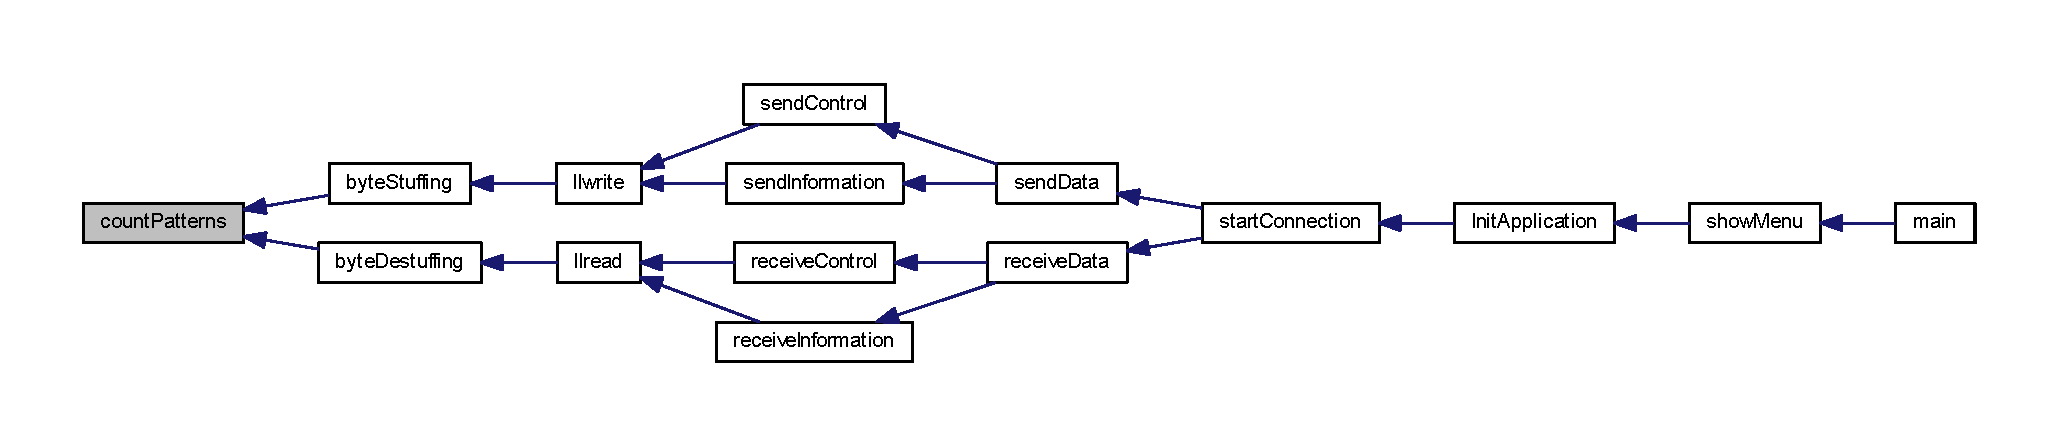
\includegraphics[width=350pt]{link_layer_8c_aa6727c503e5fa4edab84052556382a11_icgraph}
\end{center}
\end{figure}
\hypertarget{link_layer_8c_ac32e18813599af0fd5db007dbc943bd9}{}\label{link_layer_8c_ac32e18813599af0fd5db007dbc943bd9} 
\index{link\+Layer.\+c@{link\+Layer.\+c}!create\+Data\+Frame@{create\+Data\+Frame}}
\index{create\+Data\+Frame@{create\+Data\+Frame}!link\+Layer.\+c@{link\+Layer.\+c}}
\subsubsection{\texorpdfstring{create\+Data\+Frame()}{createDataFrame()}}
{\footnotesize\ttfamily unsigned char$\ast$ create\+Data\+Frame (\begin{DoxyParamCaption}\item[{unsigned char $\ast$}]{buffer,  }\item[{int}]{length }\end{DoxyParamCaption})}


\begin{DoxyParams}{Parameters}
{\em } & \\
\hline
\end{DoxyParams}
Here is the call graph for this function\+:
\nopagebreak
\begin{figure}[H]
\begin{center}
\leavevmode
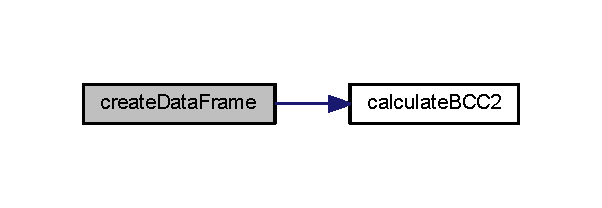
\includegraphics[width=289pt]{link_layer_8c_ac32e18813599af0fd5db007dbc943bd9_cgraph}
\end{center}
\end{figure}
Here is the caller graph for this function\+:
\nopagebreak
\begin{figure}[H]
\begin{center}
\leavevmode
\includegraphics[width=350pt]{link_layer_8c_ac32e18813599af0fd5db007dbc943bd9_icgraph}
\end{center}
\end{figure}
\hypertarget{link_layer_8c_a85cabdbf707b2b7ac21c233044d13f0e}{}\label{link_layer_8c_a85cabdbf707b2b7ac21c233044d13f0e} 
\index{link\+Layer.\+c@{link\+Layer.\+c}!get\+Baud@{get\+Baud}}
\index{get\+Baud@{get\+Baud}!link\+Layer.\+c@{link\+Layer.\+c}}
\subsubsection{\texorpdfstring{get\+Baud()}{getBaud()}}
{\footnotesize\ttfamily int get\+Baud (\begin{DoxyParamCaption}\item[{int}]{baudrate }\end{DoxyParamCaption})}

Here is the caller graph for this function\+:
\nopagebreak
\begin{figure}[H]
\begin{center}
\leavevmode
\includegraphics[width=350pt]{link_layer_8c_a85cabdbf707b2b7ac21c233044d13f0e_icgraph}
\end{center}
\end{figure}
\hypertarget{link_layer_8c_a7ff6916ccba0812bd39d4f06eb25af2c}{}\label{link_layer_8c_a7ff6916ccba0812bd39d4f06eb25af2c} 
\index{link\+Layer.\+c@{link\+Layer.\+c}!get\+Num\+Frame\+Itransmitted@{get\+Num\+Frame\+Itransmitted}}
\index{get\+Num\+Frame\+Itransmitted@{get\+Num\+Frame\+Itransmitted}!link\+Layer.\+c@{link\+Layer.\+c}}
\subsubsection{\texorpdfstring{get\+Num\+Frame\+Itransmitted()}{getNumFrameItransmitted()}}
{\footnotesize\ttfamily int get\+Num\+Frame\+Itransmitted (\begin{DoxyParamCaption}{ }\end{DoxyParamCaption})}

Here is the caller graph for this function\+:
\nopagebreak
\begin{figure}[H]
\begin{center}
\leavevmode
\includegraphics[width=350pt]{link_layer_8c_a7ff6916ccba0812bd39d4f06eb25af2c_icgraph}
\end{center}
\end{figure}
\hypertarget{link_layer_8c_a1d6d156ac0b76c0b763bd86644697c0c}{}\label{link_layer_8c_a1d6d156ac0b76c0b763bd86644697c0c} 
\index{link\+Layer.\+c@{link\+Layer.\+c}!get\+Num\+R\+EJ@{get\+Num\+R\+EJ}}
\index{get\+Num\+R\+EJ@{get\+Num\+R\+EJ}!link\+Layer.\+c@{link\+Layer.\+c}}
\subsubsection{\texorpdfstring{get\+Num\+R\+E\+J()}{getNumREJ()}}
{\footnotesize\ttfamily int get\+Num\+R\+EJ (\begin{DoxyParamCaption}{ }\end{DoxyParamCaption})}

Here is the caller graph for this function\+:
\nopagebreak
\begin{figure}[H]
\begin{center}
\leavevmode
\includegraphics[width=350pt]{link_layer_8c_a1d6d156ac0b76c0b763bd86644697c0c_icgraph}
\end{center}
\end{figure}
\hypertarget{link_layer_8c_acf7f29601204c0a58a804bcadd2e46c9}{}\label{link_layer_8c_acf7f29601204c0a58a804bcadd2e46c9} 
\index{link\+Layer.\+c@{link\+Layer.\+c}!get\+Num\+Time\+Outs@{get\+Num\+Time\+Outs}}
\index{get\+Num\+Time\+Outs@{get\+Num\+Time\+Outs}!link\+Layer.\+c@{link\+Layer.\+c}}
\subsubsection{\texorpdfstring{get\+Num\+Time\+Outs()}{getNumTimeOuts()}}
{\footnotesize\ttfamily int get\+Num\+Time\+Outs (\begin{DoxyParamCaption}{ }\end{DoxyParamCaption})}

Here is the caller graph for this function\+:
\nopagebreak
\begin{figure}[H]
\begin{center}
\leavevmode
\includegraphics[width=350pt]{link_layer_8c_acf7f29601204c0a58a804bcadd2e46c9_icgraph}
\end{center}
\end{figure}
\hypertarget{link_layer_8c_affeeaaec470b74e3d98431a3841ffc4f}{}\label{link_layer_8c_affeeaaec470b74e3d98431a3841ffc4f} 
\index{link\+Layer.\+c@{link\+Layer.\+c}!get\+Total\+I\+Transmissions@{get\+Total\+I\+Transmissions}}
\index{get\+Total\+I\+Transmissions@{get\+Total\+I\+Transmissions}!link\+Layer.\+c@{link\+Layer.\+c}}
\subsubsection{\texorpdfstring{get\+Total\+I\+Transmissions()}{getTotalITransmissions()}}
{\footnotesize\ttfamily int get\+Total\+I\+Transmissions (\begin{DoxyParamCaption}{ }\end{DoxyParamCaption})}

Here is the caller graph for this function\+:
\nopagebreak
\begin{figure}[H]
\begin{center}
\leavevmode
\includegraphics[width=350pt]{link_layer_8c_affeeaaec470b74e3d98431a3841ffc4f_icgraph}
\end{center}
\end{figure}
\hypertarget{link_layer_8c_a911024c5b110489238e2e29e119c93b0}{}\label{link_layer_8c_a911024c5b110489238e2e29e119c93b0} 
\index{link\+Layer.\+c@{link\+Layer.\+c}!init\+Link\+Layer@{init\+Link\+Layer}}
\index{init\+Link\+Layer@{init\+Link\+Layer}!link\+Layer.\+c@{link\+Layer.\+c}}
\subsubsection{\texorpdfstring{init\+Link\+Layer()}{initLinkLayer()}}
{\footnotesize\ttfamily int init\+Link\+Layer (\begin{DoxyParamCaption}\item[{int}]{port,  }\item[{int}]{status,  }\item[{int}]{baud\+Rate,  }\item[{int}]{retries,  }\item[{int}]{timeout }\end{DoxyParamCaption})}

\mbox{[}init\+Link\+Layer description\mbox{]} 
\begin{DoxyParams}{Parameters}
{\em port} & \mbox{[}description\mbox{]} \\
\hline
{\em status} & \mbox{[}description\mbox{]} \\
\hline
{\em baud\+Rate} & \mbox{[}description\mbox{]} \\
\hline
{\em package\+Size} & \mbox{[}description\mbox{]} \\
\hline
{\em retries} & \mbox{[}description\mbox{]} \\
\hline
{\em timeout} & \mbox{[}description\mbox{]} \\
\hline
\end{DoxyParams}
\begin{DoxyReturn}{Returns}
\mbox{[}description\mbox{]} 
\end{DoxyReturn}
Here is the call graph for this function\+:
\nopagebreak
\begin{figure}[H]
\begin{center}
\leavevmode
\includegraphics[width=240pt]{link_layer_8c_a911024c5b110489238e2e29e119c93b0_cgraph}
\end{center}
\end{figure}
Here is the caller graph for this function\+:
\nopagebreak
\begin{figure}[H]
\begin{center}
\leavevmode
\includegraphics[width=324pt]{link_layer_8c_a911024c5b110489238e2e29e119c93b0_icgraph}
\end{center}
\end{figure}
\hypertarget{link_layer_8c_a343e4b5928516727236a390a25f28c77}{}\label{link_layer_8c_a343e4b5928516727236a390a25f28c77} 
\index{link\+Layer.\+c@{link\+Layer.\+c}!llclose@{llclose}}
\index{llclose@{llclose}!link\+Layer.\+c@{link\+Layer.\+c}}
\subsubsection{\texorpdfstring{llclose()}{llclose()}}
{\footnotesize\ttfamily int llclose (\begin{DoxyParamCaption}\item[{int}]{fd }\end{DoxyParamCaption})}

\mbox{[}llclose description\mbox{]} 
\begin{DoxyParams}{Parameters}
{\em fd} & \mbox{[}description\mbox{]} \\
\hline
\end{DoxyParams}
\begin{DoxyReturn}{Returns}
\mbox{[}description\mbox{]} 
\end{DoxyReturn}
Here is the call graph for this function\+:
\nopagebreak
\begin{figure}[H]
\begin{center}
\leavevmode
\includegraphics[width=346pt]{link_layer_8c_a343e4b5928516727236a390a25f28c77_cgraph}
\end{center}
\end{figure}
Here is the caller graph for this function\+:
\nopagebreak
\begin{figure}[H]
\begin{center}
\leavevmode
\includegraphics[width=350pt]{link_layer_8c_a343e4b5928516727236a390a25f28c77_icgraph}
\end{center}
\end{figure}
\hypertarget{link_layer_8c_a3d8522ab922e18bc1571ae49767b55e9}{}\label{link_layer_8c_a3d8522ab922e18bc1571ae49767b55e9} 
\index{link\+Layer.\+c@{link\+Layer.\+c}!llopen@{llopen}}
\index{llopen@{llopen}!link\+Layer.\+c@{link\+Layer.\+c}}
\subsubsection{\texorpdfstring{llopen()}{llopen()}}
{\footnotesize\ttfamily int llopen (\begin{DoxyParamCaption}\item[{int}]{fd }\end{DoxyParamCaption})}

\mbox{[}llopen description\mbox{]} 
\begin{DoxyParams}{Parameters}
{\em fd} & \mbox{[}description\mbox{]} \\
\hline
\end{DoxyParams}
\begin{DoxyReturn}{Returns}
\mbox{[}description\mbox{]} 
\end{DoxyReturn}
Here is the call graph for this function\+:
\nopagebreak
\begin{figure}[H]
\begin{center}
\leavevmode
\includegraphics[width=344pt]{link_layer_8c_a3d8522ab922e18bc1571ae49767b55e9_cgraph}
\end{center}
\end{figure}
Here is the caller graph for this function\+:
\nopagebreak
\begin{figure}[H]
\begin{center}
\leavevmode
\includegraphics[width=350pt]{link_layer_8c_a3d8522ab922e18bc1571ae49767b55e9_icgraph}
\end{center}
\end{figure}
\hypertarget{link_layer_8c_a8a2fe283b8290cc1336a667a712cc187}{}\label{link_layer_8c_a8a2fe283b8290cc1336a667a712cc187} 
\index{link\+Layer.\+c@{link\+Layer.\+c}!llread@{llread}}
\index{llread@{llread}!link\+Layer.\+c@{link\+Layer.\+c}}
\subsubsection{\texorpdfstring{llread()}{llread()}}
{\footnotesize\ttfamily int llread (\begin{DoxyParamCaption}\item[{int}]{fd,  }\item[{unsigned char $\ast$}]{package,  }\item[{int}]{num\+Frame }\end{DoxyParamCaption})}

\mbox{[}llread description\mbox{]} 
\begin{DoxyParams}{Parameters}
{\em buffer} & \mbox{[}description\mbox{]} \\
\hline
\end{DoxyParams}
\begin{DoxyReturn}{Returns}
\mbox{[}description\mbox{]} 
\end{DoxyReturn}
Here is the call graph for this function\+:
\nopagebreak
\begin{figure}[H]
\begin{center}
\leavevmode
\includegraphics[width=350pt]{link_layer_8c_a8a2fe283b8290cc1336a667a712cc187_cgraph}
\end{center}
\end{figure}
Here is the caller graph for this function\+:
\nopagebreak
\begin{figure}[H]
\begin{center}
\leavevmode
\includegraphics[width=350pt]{link_layer_8c_a8a2fe283b8290cc1336a667a712cc187_icgraph}
\end{center}
\end{figure}
\hypertarget{link_layer_8c_a363d12e859b97c186f6b28c96934bad4}{}\label{link_layer_8c_a363d12e859b97c186f6b28c96934bad4} 
\index{link\+Layer.\+c@{link\+Layer.\+c}!llwrite@{llwrite}}
\index{llwrite@{llwrite}!link\+Layer.\+c@{link\+Layer.\+c}}
\subsubsection{\texorpdfstring{llwrite()}{llwrite()}}
{\footnotesize\ttfamily int llwrite (\begin{DoxyParamCaption}\item[{unsigned char $\ast$}]{buffer,  }\item[{int}]{length,  }\item[{int}]{fd }\end{DoxyParamCaption})}

\mbox{[}llwrite description\mbox{]} 
\begin{DoxyParams}{Parameters}
{\em buffer} & \mbox{[}description\mbox{]} \\
\hline
{\em length} & \mbox{[}description\mbox{]} \\
\hline
{\em fd} & \mbox{[}description\mbox{]} \\
\hline
\end{DoxyParams}
\begin{DoxyReturn}{Returns}
\mbox{[}description\mbox{]} 
\end{DoxyReturn}
Here is the call graph for this function\+:
\nopagebreak
\begin{figure}[H]
\begin{center}
\leavevmode
\includegraphics[width=350pt]{link_layer_8c_a363d12e859b97c186f6b28c96934bad4_cgraph}
\end{center}
\end{figure}
Here is the caller graph for this function\+:
\nopagebreak
\begin{figure}[H]
\begin{center}
\leavevmode
\includegraphics[width=350pt]{link_layer_8c_a363d12e859b97c186f6b28c96934bad4_icgraph}
\end{center}
\end{figure}
\hypertarget{link_layer_8c_abfbd40d058faa134b9034af9d2d865d9}{}\label{link_layer_8c_abfbd40d058faa134b9034af9d2d865d9} 
\index{link\+Layer.\+c@{link\+Layer.\+c}!read\+Data\+Frame@{read\+Data\+Frame}}
\index{read\+Data\+Frame@{read\+Data\+Frame}!link\+Layer.\+c@{link\+Layer.\+c}}
\subsubsection{\texorpdfstring{read\+Data\+Frame()}{readDataFrame()}}
{\footnotesize\ttfamily int read\+Data\+Frame (\begin{DoxyParamCaption}\item[{int}]{fd,  }\item[{unsigned char $\ast$}]{frame }\end{DoxyParamCaption})}

State machine to read the I frame frame is the buffer in which the bytes read are stored State machine to read the I frame frame is the buffer in which the bytes read are stored 
\begin{DoxyParams}{Parameters}
{\em } & \\
\hline
\end{DoxyParams}
Here is the caller graph for this function\+:
\nopagebreak
\begin{figure}[H]
\begin{center}
\leavevmode
\includegraphics[width=350pt]{link_layer_8c_abfbd40d058faa134b9034af9d2d865d9_icgraph}
\end{center}
\end{figure}
\hypertarget{link_layer_8c_af4c7f81a4d22d375976891988ef065c8}{}\label{link_layer_8c_af4c7f81a4d22d375976891988ef065c8} 
\index{link\+Layer.\+c@{link\+Layer.\+c}!send\+Supervision@{send\+Supervision}}
\index{send\+Supervision@{send\+Supervision}!link\+Layer.\+c@{link\+Layer.\+c}}
\subsubsection{\texorpdfstring{send\+Supervision()}{sendSupervision()}}
{\footnotesize\ttfamily int send\+Supervision (\begin{DoxyParamCaption}\item[{int}]{fd,  }\item[{unsigned char}]{control }\end{DoxyParamCaption})}

\mbox{[}send\+Supervision description\mbox{]} 
\begin{DoxyParams}{Parameters}
{\em fd} & \mbox{[}description\mbox{]} \\
\hline
{\em control} & \mbox{[}description\mbox{]} \\
\hline
\end{DoxyParams}
\begin{DoxyReturn}{Returns}
\mbox{[}description\mbox{]} 
\end{DoxyReturn}
Here is the caller graph for this function\+:
\nopagebreak
\begin{figure}[H]
\begin{center}
\leavevmode
\includegraphics[width=350pt]{link_layer_8c_af4c7f81a4d22d375976891988ef065c8_icgraph}
\end{center}
\end{figure}
\hypertarget{link_layer_8c_a927fcc5a512622e7fc4b688966241284}{}\label{link_layer_8c_a927fcc5a512622e7fc4b688966241284} 
\index{link\+Layer.\+c@{link\+Layer.\+c}!update\+Ns@{update\+Ns}}
\index{update\+Ns@{update\+Ns}!link\+Layer.\+c@{link\+Layer.\+c}}
\subsubsection{\texorpdfstring{update\+Ns()}{updateNs()}}
{\footnotesize\ttfamily void update\+Ns (\begin{DoxyParamCaption}{ }\end{DoxyParamCaption})}

Here is the caller graph for this function\+:
\nopagebreak
\begin{figure}[H]
\begin{center}
\leavevmode
\includegraphics[width=350pt]{link_layer_8c_a927fcc5a512622e7fc4b688966241284_icgraph}
\end{center}
\end{figure}
\hypertarget{link_layer_8c_a3a87048128ef21ca08862bf197517143}{}\label{link_layer_8c_a3a87048128ef21ca08862bf197517143} 
\index{link\+Layer.\+c@{link\+Layer.\+c}!wait\+For\+Response@{wait\+For\+Response}}
\index{wait\+For\+Response@{wait\+For\+Response}!link\+Layer.\+c@{link\+Layer.\+c}}
\subsubsection{\texorpdfstring{wait\+For\+Response()}{waitForResponse()}}
{\footnotesize\ttfamily int wait\+For\+Response (\begin{DoxyParamCaption}\item[{int}]{fd,  }\item[{unsigned char}]{flag\+Type }\end{DoxyParamCaption})}


\begin{DoxyParams}{Parameters}
{\em serial} & port descriptor \\
\hline
{\em type} & of flag sent by the emitter or the receiver \\
\hline
{\em link} & layer object \\
\hline
\end{DoxyParams}
\begin{DoxyReturn}{Returns}
0 if the flag has been read under the number of transmissions defined, -\/1 otherwise 
\end{DoxyReturn}
Here is the call graph for this function\+:
\nopagebreak
\begin{figure}[H]
\begin{center}
\leavevmode
\includegraphics[width=266pt]{link_layer_8c_a3a87048128ef21ca08862bf197517143_cgraph}
\end{center}
\end{figure}
Here is the caller graph for this function\+:
\nopagebreak
\begin{figure}[H]
\begin{center}
\leavevmode
\includegraphics[width=350pt]{link_layer_8c_a3a87048128ef21ca08862bf197517143_icgraph}
\end{center}
\end{figure}


\subsection{Variable Documentation}
\hypertarget{link_layer_8c_adf916204820072417ed73a32de1cefcf}{}\label{link_layer_8c_adf916204820072417ed73a32de1cefcf} 
\index{link\+Layer.\+c@{link\+Layer.\+c}!flag@{flag}}
\index{flag@{flag}!link\+Layer.\+c@{link\+Layer.\+c}}
\subsubsection{\texorpdfstring{flag}{flag}}
{\footnotesize\ttfamily int flag = 1}

\hypertarget{link_layer_8c_a70df012765479ea774aa425d7527e718}{}\label{link_layer_8c_a70df012765479ea774aa425d7527e718} 
\index{link\+Layer.\+c@{link\+Layer.\+c}!link\+Layer@{link\+Layer}}
\index{link\+Layer@{link\+Layer}!link\+Layer.\+c@{link\+Layer.\+c}}
\subsubsection{\texorpdfstring{link\+Layer}{linkLayer}}
{\footnotesize\ttfamily \hyperlink{struct_link_layer}{Link\+Layer}$\ast$ link\+Layer}

\hypertarget{link_layer_8c_a149b5ea0e56df54ba2f74166453a8fd9}{}\label{link_layer_8c_a149b5ea0e56df54ba2f74166453a8fd9} 
\index{link\+Layer.\+c@{link\+Layer.\+c}!num\+FrameI@{num\+FrameI}}
\index{num\+FrameI@{num\+FrameI}!link\+Layer.\+c@{link\+Layer.\+c}}
\subsubsection{\texorpdfstring{num\+FrameI}{numFrameI}}
{\footnotesize\ttfamily int num\+FrameI = 0}

\hypertarget{link_layer_8c_a0637f6d853eaa5a7e5bead66bc9ee567}{}\label{link_layer_8c_a0637f6d853eaa5a7e5bead66bc9ee567} 
\index{link\+Layer.\+c@{link\+Layer.\+c}!num\+Frame\+Itransmitted@{num\+Frame\+Itransmitted}}
\index{num\+Frame\+Itransmitted@{num\+Frame\+Itransmitted}!link\+Layer.\+c@{link\+Layer.\+c}}
\subsubsection{\texorpdfstring{num\+Frame\+Itransmitted}{numFrameItransmitted}}
{\footnotesize\ttfamily int num\+Frame\+Itransmitted = 0}

\hypertarget{link_layer_8c_a08882678e9b70455b991496b0bf0f55b}{}\label{link_layer_8c_a08882678e9b70455b991496b0bf0f55b} 
\index{link\+Layer.\+c@{link\+Layer.\+c}!num\+R\+E\+Jreceived@{num\+R\+E\+Jreceived}}
\index{num\+R\+E\+Jreceived@{num\+R\+E\+Jreceived}!link\+Layer.\+c@{link\+Layer.\+c}}
\subsubsection{\texorpdfstring{num\+R\+E\+Jreceived}{numREJreceived}}
{\footnotesize\ttfamily int num\+R\+E\+Jreceived = 0}

\hypertarget{link_layer_8c_ad28672c114a1578ed97b0a73abbdc761}{}\label{link_layer_8c_ad28672c114a1578ed97b0a73abbdc761} 
\index{link\+Layer.\+c@{link\+Layer.\+c}!num\+Time\+Outs@{num\+Time\+Outs}}
\index{num\+Time\+Outs@{num\+Time\+Outs}!link\+Layer.\+c@{link\+Layer.\+c}}
\subsubsection{\texorpdfstring{num\+Time\+Outs}{numTimeOuts}}
{\footnotesize\ttfamily int num\+Time\+Outs = 0}

\hypertarget{link_layer_8c_a5fbc721140a2ca81a3fcbdafaa668bdd}{}\label{link_layer_8c_a5fbc721140a2ca81a3fcbdafaa668bdd} 
\index{link\+Layer.\+c@{link\+Layer.\+c}!S\+T\+OP@{S\+T\+OP}}
\index{S\+T\+OP@{S\+T\+OP}!link\+Layer.\+c@{link\+Layer.\+c}}
\subsubsection{\texorpdfstring{S\+T\+OP}{STOP}}
{\footnotesize\ttfamily volatile int S\+T\+OP =\hyperlink{link_layer_8h_aa93f0eb578d23995850d61f7d61c55c1}{F\+A\+L\+SE}}

\hypertarget{link_layer_8c_ae2c6087027bfdf561a2b766975b47ee8}{}\label{link_layer_8c_ae2c6087027bfdf561a2b766975b47ee8} 
\index{link\+Layer.\+c@{link\+Layer.\+c}!timer@{timer}}
\index{timer@{timer}!link\+Layer.\+c@{link\+Layer.\+c}}
\subsubsection{\texorpdfstring{timer}{timer}}
{\footnotesize\ttfamily int timer = 1}


\hypertarget{link_layer_8h}{}\section{link\+Layer.\+h File Reference}
\label{link_layer_8h}\index{link\+Layer.\+h@{link\+Layer.\+h}}
{\ttfamily \#include $<$sys/types.\+h$>$}\newline
{\ttfamily \#include $<$sys/stat.\+h$>$}\newline
{\ttfamily \#include $<$fcntl.\+h$>$}\newline
{\ttfamily \#include $<$termios.\+h$>$}\newline
{\ttfamily \#include $<$stdio.\+h$>$}\newline
{\ttfamily \#include $<$stdlib.\+h$>$}\newline
{\ttfamily \#include $<$strings.\+h$>$}\newline
{\ttfamily \#include $<$string.\+h$>$}\newline
{\ttfamily \#include $<$unistd.\+h$>$}\newline
{\ttfamily \#include $<$signal.\+h$>$}\newline
Include dependency graph for link\+Layer.\+h\+:\nopagebreak
\begin{figure}[H]
\begin{center}
\leavevmode
\includegraphics[width=350pt]{link_layer_8h__incl}
\end{center}
\end{figure}
This graph shows which files directly or indirectly include this file\+:\nopagebreak
\begin{figure}[H]
\begin{center}
\leavevmode
\includegraphics[width=302pt]{link_layer_8h__dep__incl}
\end{center}
\end{figure}
\subsection*{Data Structures}
\begin{DoxyCompactItemize}
\item 
struct \hyperlink{struct_link_layer}{Link\+Layer}
\end{DoxyCompactItemize}
\subsection*{Macros}
\begin{DoxyCompactItemize}
\item 
\#define \hyperlink{link_layer_8h_aecae779890dfc6b313fe2854369e5497}{M\+A\+X\+\_\+\+F\+R\+A\+M\+E\+\_\+\+L\+E\+N\+G\+TH}~1024
\item 
\#define \hyperlink{link_layer_8h_aa93f0eb578d23995850d61f7d61c55c1}{F\+A\+L\+SE}~0
\item 
\#define \hyperlink{link_layer_8h_aa8cecfc5c5c054d2875c03e77b7be15d}{T\+R\+UE}~1
\item 
\#define \hyperlink{link_layer_8h_afe4b0e625372cd38ec60150d6f5594b8}{E\+S\+C\+A\+PE}~0x7d
\item 
\#define \hyperlink{link_layer_8h_af8bfae90c5d6853fcfb487e05b9f50c8}{F\+L\+AG}~0x7e
\item 
\#define \hyperlink{link_layer_8h_a955f504eccf76b4eb2489c0adab03121}{A}~0x03
\item 
\#define \hyperlink{link_layer_8h_a480bc08be2722ba0343812c003604392}{C\+\_\+\+S\+ET}~0x03
\item 
\#define \hyperlink{link_layer_8h_aba4eb3c08ee682afce79d9b93c2edbb6}{C\+\_\+\+UA}~0x07
\item 
\#define \hyperlink{link_layer_8h_a1b236657857dbb3ef5a6d98ac23d8274}{C\+\_\+I}~0x00
\item 
\#define \hyperlink{link_layer_8h_a6a2ca6d1d21a06b77cc24fa010b182fc}{C\+\_\+\+RR}~0x85
\item 
\#define \hyperlink{link_layer_8h_aa8684947a54e16bc93295e9638edea16}{C\+\_\+\+D\+I\+SC}~0x0b
\item 
\#define \hyperlink{link_layer_8h_a0286c298adb21144b48363807c8c0065}{C\+\_\+\+R\+EJ}~0x81
\item 
\#define \hyperlink{link_layer_8h_afe2d6d328de9aa79a2a8c0ec73554012}{UA}~0
\item 
\#define \hyperlink{link_layer_8h_a63979cf6054f403eab1d354e6dcc4ce9}{RR}~1
\item 
\#define \hyperlink{link_layer_8h_a96618cbf2cadbdcf5f58be1203229fa0}{D\+I\+SC}~2
\item 
\#define \hyperlink{link_layer_8h_a59da1d65e87a723efe808dbabb4fc205}{S\+ET}~3
\item 
\#define \hyperlink{link_layer_8h_af3a83c322d5c4e3f87d1bf1079c31523}{B\+I\+T\+\_\+\+M\+A\+SK}(bit)~(1 $<$$<$ (bit))
\item 
\#define \hyperlink{link_layer_8h_a45b00778710610a16c2b99be70a1be0d}{T\+O\+O\+G\+L\+E\+\_\+\+B\+IT}(value,  bit)~((value) $^\wedge$= \hyperlink{link_layer_8h_af3a83c322d5c4e3f87d1bf1079c31523}{B\+I\+T\+\_\+\+M\+A\+SK}(bit))
\end{DoxyCompactItemize}
\subsection*{Typedefs}
\begin{DoxyCompactItemize}
\item 
typedef struct \hyperlink{struct_link_layer}{Link\+Layer} \hyperlink{link_layer_8h_a83ff6d9b6ecad8dd99f63cc48ac5abe8}{Link\+Layer}
\end{DoxyCompactItemize}
\subsection*{Functions}
\begin{DoxyCompactItemize}
\item 
int \hyperlink{link_layer_8h_a7cf6ec35c966c219876457f68371d8b7}{init\+Link\+Layer} (int port, int status, int \hyperlink{main_8c_a352a05efbed742a2c47e738725ee5613}{baud\+Rate}, int \hyperlink{main_8c_a8ba735ab56b2afeb844916994c86f3f5}{retries}, int timeout)
\item 
int \hyperlink{link_layer_8h_a3d8522ab922e18bc1571ae49767b55e9}{llopen} (int fd)
\item 
int \hyperlink{link_layer_8h_a363d12e859b97c186f6b28c96934bad4}{llwrite} (unsigned char $\ast$buffer, int length, int fd)
\item 
int \hyperlink{link_layer_8h_a8a2fe283b8290cc1336a667a712cc187}{llread} (int fd, unsigned char $\ast$package, int num\+Frame)
\item 
int \hyperlink{link_layer_8h_a343e4b5928516727236a390a25f28c77}{llclose} (int fd)
\item 
int \hyperlink{link_layer_8h_a9a0e32fb00e3aca10cbf4f35431eb39a}{estabilish\+Connection} (int fd)
\item 
int \hyperlink{link_layer_8h_ae0c743b77cc7b557adc8d8468275289a}{end\+Connection} (int fd)
\item 
int \hyperlink{link_layer_8h_af4c7f81a4d22d375976891988ef065c8}{send\+Supervision} (int fd, unsigned char control)
\item 
int \hyperlink{link_layer_8h_a7ecc5cd3d4867926b1df6783e1214de1}{write\+RR} (int fd)
\item 
int \hyperlink{link_layer_8h_a3a87048128ef21ca08862bf197517143}{wait\+For\+Response} (int fd, unsigned char flag\+Type)
\item 
int \hyperlink{link_layer_8h_aa6727c503e5fa4edab84052556382a11}{count\+Patterns} (unsigned char $\ast$$\ast$frame, int length)
\item 
int \hyperlink{link_layer_8h_a1295fa2e6765acc35b05d8cb9dc9e9a1}{byte\+Stuffing} (unsigned char $\ast$$\ast$frame, int length)
\item 
int \hyperlink{link_layer_8h_a888914efd19822deb27e1f0a5cacca94}{byte\+Destuffing} (unsigned char $\ast$$\ast$frame, int length)
\item 
void \hyperlink{link_layer_8h_adc4d249c47efd1729a17f2782de863c2}{atende} ()
\item 
unsigned char \hyperlink{link_layer_8h_aaa527233d90b0499478a918eea3f1d19}{calculate\+B\+C\+C2} (unsigned char $\ast$frame, int length)
\item 
unsigned char $\ast$ \hyperlink{link_layer_8h_ac32e18813599af0fd5db007dbc943bd9}{create\+Data\+Frame} (unsigned char $\ast$buffer, int length)
\item 
int \hyperlink{link_layer_8h_afbf51aa3d02b21b8cfa10238e0bfc626}{read\+Data\+Information} (char $\ast$frame, char byte\+Read)
\item 
int \hyperlink{link_layer_8h_abfbd40d058faa134b9034af9d2d865d9}{read\+Data\+Frame} (int fd, unsigned char $\ast$frame)
\item 
int \hyperlink{link_layer_8h_a520783778c9b115983967fe315306e36}{check\+For\+Frame\+Errors} (int fd, unsigned char $\ast$buffer, unsigned char $\ast$package, int length, int data\+Size)
\item 
void \hyperlink{link_layer_8h_a927fcc5a512622e7fc4b688966241284}{update\+Ns} ()
\item 
int \hyperlink{link_layer_8h_a85cabdbf707b2b7ac21c233044d13f0e}{get\+Baud} (int baudrate)
\item 
int \hyperlink{link_layer_8h_a1d6d156ac0b76c0b763bd86644697c0c}{get\+Num\+R\+EJ} ()
\item 
int \hyperlink{link_layer_8h_affeeaaec470b74e3d98431a3841ffc4f}{get\+Total\+I\+Transmissions} ()
\item 
int \hyperlink{link_layer_8h_a7ff6916ccba0812bd39d4f06eb25af2c}{get\+Num\+Frame\+Itransmitted} ()
\item 
int \hyperlink{link_layer_8h_acf7f29601204c0a58a804bcadd2e46c9}{get\+Num\+Time\+Outs} ()
\end{DoxyCompactItemize}


\subsection{Macro Definition Documentation}
\hypertarget{link_layer_8h_a955f504eccf76b4eb2489c0adab03121}{}\label{link_layer_8h_a955f504eccf76b4eb2489c0adab03121} 
\index{link\+Layer.\+h@{link\+Layer.\+h}!A@{A}}
\index{A@{A}!link\+Layer.\+h@{link\+Layer.\+h}}
\subsubsection{\texorpdfstring{A}{A}}
{\footnotesize\ttfamily \#define A~0x03}

\hypertarget{link_layer_8h_af3a83c322d5c4e3f87d1bf1079c31523}{}\label{link_layer_8h_af3a83c322d5c4e3f87d1bf1079c31523} 
\index{link\+Layer.\+h@{link\+Layer.\+h}!B\+I\+T\+\_\+\+M\+A\+SK@{B\+I\+T\+\_\+\+M\+A\+SK}}
\index{B\+I\+T\+\_\+\+M\+A\+SK@{B\+I\+T\+\_\+\+M\+A\+SK}!link\+Layer.\+h@{link\+Layer.\+h}}
\subsubsection{\texorpdfstring{B\+I\+T\+\_\+\+M\+A\+SK}{BIT\_MASK}}
{\footnotesize\ttfamily \#define B\+I\+T\+\_\+\+M\+A\+SK(\begin{DoxyParamCaption}\item[{}]{bit }\end{DoxyParamCaption})~(1 $<$$<$ (bit))}

\hypertarget{link_layer_8h_aa8684947a54e16bc93295e9638edea16}{}\label{link_layer_8h_aa8684947a54e16bc93295e9638edea16} 
\index{link\+Layer.\+h@{link\+Layer.\+h}!C\+\_\+\+D\+I\+SC@{C\+\_\+\+D\+I\+SC}}
\index{C\+\_\+\+D\+I\+SC@{C\+\_\+\+D\+I\+SC}!link\+Layer.\+h@{link\+Layer.\+h}}
\subsubsection{\texorpdfstring{C\+\_\+\+D\+I\+SC}{C\_DISC}}
{\footnotesize\ttfamily \#define C\+\_\+\+D\+I\+SC~0x0b}

\hypertarget{link_layer_8h_a1b236657857dbb3ef5a6d98ac23d8274}{}\label{link_layer_8h_a1b236657857dbb3ef5a6d98ac23d8274} 
\index{link\+Layer.\+h@{link\+Layer.\+h}!C\+\_\+I@{C\+\_\+I}}
\index{C\+\_\+I@{C\+\_\+I}!link\+Layer.\+h@{link\+Layer.\+h}}
\subsubsection{\texorpdfstring{C\+\_\+I}{C\_I}}
{\footnotesize\ttfamily \#define C\+\_\+I~0x00}

\hypertarget{link_layer_8h_a0286c298adb21144b48363807c8c0065}{}\label{link_layer_8h_a0286c298adb21144b48363807c8c0065} 
\index{link\+Layer.\+h@{link\+Layer.\+h}!C\+\_\+\+R\+EJ@{C\+\_\+\+R\+EJ}}
\index{C\+\_\+\+R\+EJ@{C\+\_\+\+R\+EJ}!link\+Layer.\+h@{link\+Layer.\+h}}
\subsubsection{\texorpdfstring{C\+\_\+\+R\+EJ}{C\_REJ}}
{\footnotesize\ttfamily \#define C\+\_\+\+R\+EJ~0x81}

\hypertarget{link_layer_8h_a6a2ca6d1d21a06b77cc24fa010b182fc}{}\label{link_layer_8h_a6a2ca6d1d21a06b77cc24fa010b182fc} 
\index{link\+Layer.\+h@{link\+Layer.\+h}!C\+\_\+\+RR@{C\+\_\+\+RR}}
\index{C\+\_\+\+RR@{C\+\_\+\+RR}!link\+Layer.\+h@{link\+Layer.\+h}}
\subsubsection{\texorpdfstring{C\+\_\+\+RR}{C\_RR}}
{\footnotesize\ttfamily \#define C\+\_\+\+RR~0x85}

\hypertarget{link_layer_8h_a480bc08be2722ba0343812c003604392}{}\label{link_layer_8h_a480bc08be2722ba0343812c003604392} 
\index{link\+Layer.\+h@{link\+Layer.\+h}!C\+\_\+\+S\+ET@{C\+\_\+\+S\+ET}}
\index{C\+\_\+\+S\+ET@{C\+\_\+\+S\+ET}!link\+Layer.\+h@{link\+Layer.\+h}}
\subsubsection{\texorpdfstring{C\+\_\+\+S\+ET}{C\_SET}}
{\footnotesize\ttfamily \#define C\+\_\+\+S\+ET~0x03}

\hypertarget{link_layer_8h_aba4eb3c08ee682afce79d9b93c2edbb6}{}\label{link_layer_8h_aba4eb3c08ee682afce79d9b93c2edbb6} 
\index{link\+Layer.\+h@{link\+Layer.\+h}!C\+\_\+\+UA@{C\+\_\+\+UA}}
\index{C\+\_\+\+UA@{C\+\_\+\+UA}!link\+Layer.\+h@{link\+Layer.\+h}}
\subsubsection{\texorpdfstring{C\+\_\+\+UA}{C\_UA}}
{\footnotesize\ttfamily \#define C\+\_\+\+UA~0x07}

\hypertarget{link_layer_8h_a96618cbf2cadbdcf5f58be1203229fa0}{}\label{link_layer_8h_a96618cbf2cadbdcf5f58be1203229fa0} 
\index{link\+Layer.\+h@{link\+Layer.\+h}!D\+I\+SC@{D\+I\+SC}}
\index{D\+I\+SC@{D\+I\+SC}!link\+Layer.\+h@{link\+Layer.\+h}}
\subsubsection{\texorpdfstring{D\+I\+SC}{DISC}}
{\footnotesize\ttfamily \#define D\+I\+SC~2}

\hypertarget{link_layer_8h_afe4b0e625372cd38ec60150d6f5594b8}{}\label{link_layer_8h_afe4b0e625372cd38ec60150d6f5594b8} 
\index{link\+Layer.\+h@{link\+Layer.\+h}!E\+S\+C\+A\+PE@{E\+S\+C\+A\+PE}}
\index{E\+S\+C\+A\+PE@{E\+S\+C\+A\+PE}!link\+Layer.\+h@{link\+Layer.\+h}}
\subsubsection{\texorpdfstring{E\+S\+C\+A\+PE}{ESCAPE}}
{\footnotesize\ttfamily \#define E\+S\+C\+A\+PE~0x7d}

\hypertarget{link_layer_8h_aa93f0eb578d23995850d61f7d61c55c1}{}\label{link_layer_8h_aa93f0eb578d23995850d61f7d61c55c1} 
\index{link\+Layer.\+h@{link\+Layer.\+h}!F\+A\+L\+SE@{F\+A\+L\+SE}}
\index{F\+A\+L\+SE@{F\+A\+L\+SE}!link\+Layer.\+h@{link\+Layer.\+h}}
\subsubsection{\texorpdfstring{F\+A\+L\+SE}{FALSE}}
{\footnotesize\ttfamily \#define F\+A\+L\+SE~0}

\hypertarget{link_layer_8h_af8bfae90c5d6853fcfb487e05b9f50c8}{}\label{link_layer_8h_af8bfae90c5d6853fcfb487e05b9f50c8} 
\index{link\+Layer.\+h@{link\+Layer.\+h}!F\+L\+AG@{F\+L\+AG}}
\index{F\+L\+AG@{F\+L\+AG}!link\+Layer.\+h@{link\+Layer.\+h}}
\subsubsection{\texorpdfstring{F\+L\+AG}{FLAG}}
{\footnotesize\ttfamily \#define F\+L\+AG~0x7e}

\hypertarget{link_layer_8h_aecae779890dfc6b313fe2854369e5497}{}\label{link_layer_8h_aecae779890dfc6b313fe2854369e5497} 
\index{link\+Layer.\+h@{link\+Layer.\+h}!M\+A\+X\+\_\+\+F\+R\+A\+M\+E\+\_\+\+L\+E\+N\+G\+TH@{M\+A\+X\+\_\+\+F\+R\+A\+M\+E\+\_\+\+L\+E\+N\+G\+TH}}
\index{M\+A\+X\+\_\+\+F\+R\+A\+M\+E\+\_\+\+L\+E\+N\+G\+TH@{M\+A\+X\+\_\+\+F\+R\+A\+M\+E\+\_\+\+L\+E\+N\+G\+TH}!link\+Layer.\+h@{link\+Layer.\+h}}
\subsubsection{\texorpdfstring{M\+A\+X\+\_\+\+F\+R\+A\+M\+E\+\_\+\+L\+E\+N\+G\+TH}{MAX\_FRAME\_LENGTH}}
{\footnotesize\ttfamily \#define M\+A\+X\+\_\+\+F\+R\+A\+M\+E\+\_\+\+L\+E\+N\+G\+TH~1024}

\hypertarget{link_layer_8h_a63979cf6054f403eab1d354e6dcc4ce9}{}\label{link_layer_8h_a63979cf6054f403eab1d354e6dcc4ce9} 
\index{link\+Layer.\+h@{link\+Layer.\+h}!RR@{RR}}
\index{RR@{RR}!link\+Layer.\+h@{link\+Layer.\+h}}
\subsubsection{\texorpdfstring{RR}{RR}}
{\footnotesize\ttfamily \#define RR~1}

\hypertarget{link_layer_8h_a59da1d65e87a723efe808dbabb4fc205}{}\label{link_layer_8h_a59da1d65e87a723efe808dbabb4fc205} 
\index{link\+Layer.\+h@{link\+Layer.\+h}!S\+ET@{S\+ET}}
\index{S\+ET@{S\+ET}!link\+Layer.\+h@{link\+Layer.\+h}}
\subsubsection{\texorpdfstring{S\+ET}{SET}}
{\footnotesize\ttfamily \#define S\+ET~3}

\hypertarget{link_layer_8h_a45b00778710610a16c2b99be70a1be0d}{}\label{link_layer_8h_a45b00778710610a16c2b99be70a1be0d} 
\index{link\+Layer.\+h@{link\+Layer.\+h}!T\+O\+O\+G\+L\+E\+\_\+\+B\+IT@{T\+O\+O\+G\+L\+E\+\_\+\+B\+IT}}
\index{T\+O\+O\+G\+L\+E\+\_\+\+B\+IT@{T\+O\+O\+G\+L\+E\+\_\+\+B\+IT}!link\+Layer.\+h@{link\+Layer.\+h}}
\subsubsection{\texorpdfstring{T\+O\+O\+G\+L\+E\+\_\+\+B\+IT}{TOOGLE\_BIT}}
{\footnotesize\ttfamily \#define T\+O\+O\+G\+L\+E\+\_\+\+B\+IT(\begin{DoxyParamCaption}\item[{}]{value,  }\item[{}]{bit }\end{DoxyParamCaption})~((value) $^\wedge$= \hyperlink{link_layer_8h_af3a83c322d5c4e3f87d1bf1079c31523}{B\+I\+T\+\_\+\+M\+A\+SK}(bit))}

\hypertarget{link_layer_8h_aa8cecfc5c5c054d2875c03e77b7be15d}{}\label{link_layer_8h_aa8cecfc5c5c054d2875c03e77b7be15d} 
\index{link\+Layer.\+h@{link\+Layer.\+h}!T\+R\+UE@{T\+R\+UE}}
\index{T\+R\+UE@{T\+R\+UE}!link\+Layer.\+h@{link\+Layer.\+h}}
\subsubsection{\texorpdfstring{T\+R\+UE}{TRUE}}
{\footnotesize\ttfamily \#define T\+R\+UE~1}

\hypertarget{link_layer_8h_afe2d6d328de9aa79a2a8c0ec73554012}{}\label{link_layer_8h_afe2d6d328de9aa79a2a8c0ec73554012} 
\index{link\+Layer.\+h@{link\+Layer.\+h}!UA@{UA}}
\index{UA@{UA}!link\+Layer.\+h@{link\+Layer.\+h}}
\subsubsection{\texorpdfstring{UA}{UA}}
{\footnotesize\ttfamily \#define UA~0}



\subsection{Typedef Documentation}
\hypertarget{link_layer_8h_a83ff6d9b6ecad8dd99f63cc48ac5abe8}{}\label{link_layer_8h_a83ff6d9b6ecad8dd99f63cc48ac5abe8} 
\index{link\+Layer.\+h@{link\+Layer.\+h}!Link\+Layer@{Link\+Layer}}
\index{Link\+Layer@{Link\+Layer}!link\+Layer.\+h@{link\+Layer.\+h}}
\subsubsection{\texorpdfstring{Link\+Layer}{LinkLayer}}
{\footnotesize\ttfamily typedef struct \hyperlink{struct_link_layer}{Link\+Layer} \hyperlink{struct_link_layer}{Link\+Layer}}



\subsection{Function Documentation}
\hypertarget{link_layer_8h_adc4d249c47efd1729a17f2782de863c2}{}\label{link_layer_8h_adc4d249c47efd1729a17f2782de863c2} 
\index{link\+Layer.\+h@{link\+Layer.\+h}!atende@{atende}}
\index{atende@{atende}!link\+Layer.\+h@{link\+Layer.\+h}}
\subsubsection{\texorpdfstring{atende()}{atende()}}
{\footnotesize\ttfamily void atende (\begin{DoxyParamCaption}{ }\end{DoxyParamCaption})}

Here is the caller graph for this function\+:\nopagebreak
\begin{figure}[H]
\begin{center}
\leavevmode
\includegraphics[width=350pt]{link_layer_8h_adc4d249c47efd1729a17f2782de863c2_icgraph}
\end{center}
\end{figure}
\hypertarget{link_layer_8h_a888914efd19822deb27e1f0a5cacca94}{}\label{link_layer_8h_a888914efd19822deb27e1f0a5cacca94} 
\index{link\+Layer.\+h@{link\+Layer.\+h}!byte\+Destuffing@{byte\+Destuffing}}
\index{byte\+Destuffing@{byte\+Destuffing}!link\+Layer.\+h@{link\+Layer.\+h}}
\subsubsection{\texorpdfstring{byte\+Destuffing()}{byteDestuffing()}}
{\footnotesize\ttfamily int byte\+Destuffing (\begin{DoxyParamCaption}\item[{unsigned char $\ast$$\ast$}]{frame,  }\item[{int}]{length }\end{DoxyParamCaption})}


\begin{DoxyParams}{Parameters}
{\em } & \\
\hline
\end{DoxyParams}
Here is the call graph for this function\+:\nopagebreak
\begin{figure}[H]
\begin{center}
\leavevmode
\includegraphics[width=271pt]{link_layer_8h_a888914efd19822deb27e1f0a5cacca94_cgraph}
\end{center}
\end{figure}
Here is the caller graph for this function\+:\nopagebreak
\begin{figure}[H]
\begin{center}
\leavevmode
\includegraphics[width=350pt]{link_layer_8h_a888914efd19822deb27e1f0a5cacca94_icgraph}
\end{center}
\end{figure}
\hypertarget{link_layer_8h_a1295fa2e6765acc35b05d8cb9dc9e9a1}{}\label{link_layer_8h_a1295fa2e6765acc35b05d8cb9dc9e9a1} 
\index{link\+Layer.\+h@{link\+Layer.\+h}!byte\+Stuffing@{byte\+Stuffing}}
\index{byte\+Stuffing@{byte\+Stuffing}!link\+Layer.\+h@{link\+Layer.\+h}}
\subsubsection{\texorpdfstring{byte\+Stuffing()}{byteStuffing()}}
{\footnotesize\ttfamily int byte\+Stuffing (\begin{DoxyParamCaption}\item[{unsigned char $\ast$$\ast$}]{frame,  }\item[{int}]{length }\end{DoxyParamCaption})}


\begin{DoxyParams}{Parameters}
{\em } & \\
\hline
\end{DoxyParams}
Here is the call graph for this function\+:\nopagebreak
\begin{figure}[H]
\begin{center}
\leavevmode
\includegraphics[width=261pt]{link_layer_8h_a1295fa2e6765acc35b05d8cb9dc9e9a1_cgraph}
\end{center}
\end{figure}
Here is the caller graph for this function\+:\nopagebreak
\begin{figure}[H]
\begin{center}
\leavevmode
\includegraphics[width=350pt]{link_layer_8h_a1295fa2e6765acc35b05d8cb9dc9e9a1_icgraph}
\end{center}
\end{figure}
\hypertarget{link_layer_8h_aaa527233d90b0499478a918eea3f1d19}{}\label{link_layer_8h_aaa527233d90b0499478a918eea3f1d19} 
\index{link\+Layer.\+h@{link\+Layer.\+h}!calculate\+B\+C\+C2@{calculate\+B\+C\+C2}}
\index{calculate\+B\+C\+C2@{calculate\+B\+C\+C2}!link\+Layer.\+h@{link\+Layer.\+h}}
\subsubsection{\texorpdfstring{calculate\+B\+C\+C2()}{calculateBCC2()}}
{\footnotesize\ttfamily unsigned char calculate\+B\+C\+C2 (\begin{DoxyParamCaption}\item[{unsigned char $\ast$}]{frame,  }\item[{int}]{length }\end{DoxyParamCaption})}

Calculates the X\+OR of the data bytes 
\begin{DoxyParams}{Parameters}
{\em } & \\
\hline
\end{DoxyParams}
Here is the caller graph for this function\+:\nopagebreak
\begin{figure}[H]
\begin{center}
\leavevmode
\includegraphics[width=350pt]{link_layer_8h_aaa527233d90b0499478a918eea3f1d19_icgraph}
\end{center}
\end{figure}
\hypertarget{link_layer_8h_a520783778c9b115983967fe315306e36}{}\label{link_layer_8h_a520783778c9b115983967fe315306e36} 
\index{link\+Layer.\+h@{link\+Layer.\+h}!check\+For\+Frame\+Errors@{check\+For\+Frame\+Errors}}
\index{check\+For\+Frame\+Errors@{check\+For\+Frame\+Errors}!link\+Layer.\+h@{link\+Layer.\+h}}
\subsubsection{\texorpdfstring{check\+For\+Frame\+Errors()}{checkForFrameErrors()}}
{\footnotesize\ttfamily int check\+For\+Frame\+Errors (\begin{DoxyParamCaption}\item[{int}]{fd,  }\item[{unsigned char $\ast$}]{buffer,  }\item[{unsigned char $\ast$}]{package,  }\item[{int}]{length,  }\item[{int}]{data\+Size }\end{DoxyParamCaption})}

Here is the call graph for this function\+:\nopagebreak
\begin{figure}[H]
\begin{center}
\leavevmode
\includegraphics[width=314pt]{link_layer_8h_a520783778c9b115983967fe315306e36_cgraph}
\end{center}
\end{figure}
Here is the caller graph for this function\+:\nopagebreak
\begin{figure}[H]
\begin{center}
\leavevmode
\includegraphics[width=350pt]{link_layer_8h_a520783778c9b115983967fe315306e36_icgraph}
\end{center}
\end{figure}
\hypertarget{link_layer_8h_aa6727c503e5fa4edab84052556382a11}{}\label{link_layer_8h_aa6727c503e5fa4edab84052556382a11} 
\index{link\+Layer.\+h@{link\+Layer.\+h}!count\+Patterns@{count\+Patterns}}
\index{count\+Patterns@{count\+Patterns}!link\+Layer.\+h@{link\+Layer.\+h}}
\subsubsection{\texorpdfstring{count\+Patterns()}{countPatterns()}}
{\footnotesize\ttfamily int count\+Patterns (\begin{DoxyParamCaption}\item[{unsigned char $\ast$$\ast$}]{frame,  }\item[{int}]{length }\end{DoxyParamCaption})}


\begin{DoxyParams}{Parameters}
{\em } & \\
\hline
\end{DoxyParams}
Here is the caller graph for this function\+:\nopagebreak
\begin{figure}[H]
\begin{center}
\leavevmode
\includegraphics[width=350pt]{link_layer_8h_aa6727c503e5fa4edab84052556382a11_icgraph}
\end{center}
\end{figure}
\hypertarget{link_layer_8h_ac32e18813599af0fd5db007dbc943bd9}{}\label{link_layer_8h_ac32e18813599af0fd5db007dbc943bd9} 
\index{link\+Layer.\+h@{link\+Layer.\+h}!create\+Data\+Frame@{create\+Data\+Frame}}
\index{create\+Data\+Frame@{create\+Data\+Frame}!link\+Layer.\+h@{link\+Layer.\+h}}
\subsubsection{\texorpdfstring{create\+Data\+Frame()}{createDataFrame()}}
{\footnotesize\ttfamily unsigned char$\ast$ create\+Data\+Frame (\begin{DoxyParamCaption}\item[{unsigned char $\ast$}]{buffer,  }\item[{int}]{length }\end{DoxyParamCaption})}


\begin{DoxyParams}{Parameters}
{\em } & \\
\hline
\end{DoxyParams}
Here is the call graph for this function\+:\nopagebreak
\begin{figure}[H]
\begin{center}
\leavevmode
\includegraphics[width=289pt]{link_layer_8h_ac32e18813599af0fd5db007dbc943bd9_cgraph}
\end{center}
\end{figure}
Here is the caller graph for this function\+:\nopagebreak
\begin{figure}[H]
\begin{center}
\leavevmode
\includegraphics[width=350pt]{link_layer_8h_ac32e18813599af0fd5db007dbc943bd9_icgraph}
\end{center}
\end{figure}
\hypertarget{link_layer_8h_ae0c743b77cc7b557adc8d8468275289a}{}\label{link_layer_8h_ae0c743b77cc7b557adc8d8468275289a} 
\index{link\+Layer.\+h@{link\+Layer.\+h}!end\+Connection@{end\+Connection}}
\index{end\+Connection@{end\+Connection}!link\+Layer.\+h@{link\+Layer.\+h}}
\subsubsection{\texorpdfstring{end\+Connection()}{endConnection()}}
{\footnotesize\ttfamily int end\+Connection (\begin{DoxyParamCaption}\item[{int}]{fd }\end{DoxyParamCaption})}

\mbox{[}end\+Connection description\mbox{]} 
\begin{DoxyParams}{Parameters}
{\em fd} & \mbox{[}description\mbox{]} \\
\hline
\end{DoxyParams}
\begin{DoxyReturn}{Returns}
\mbox{[}description\mbox{]} 
\end{DoxyReturn}
\hypertarget{link_layer_8h_a9a0e32fb00e3aca10cbf4f35431eb39a}{}\label{link_layer_8h_a9a0e32fb00e3aca10cbf4f35431eb39a} 
\index{link\+Layer.\+h@{link\+Layer.\+h}!estabilish\+Connection@{estabilish\+Connection}}
\index{estabilish\+Connection@{estabilish\+Connection}!link\+Layer.\+h@{link\+Layer.\+h}}
\subsubsection{\texorpdfstring{estabilish\+Connection()}{estabilishConnection()}}
{\footnotesize\ttfamily int estabilish\+Connection (\begin{DoxyParamCaption}\item[{int}]{fd }\end{DoxyParamCaption})}

\mbox{[}estabilish\+Connection description\mbox{]} 
\begin{DoxyParams}{Parameters}
{\em fd} & \mbox{[}description\mbox{]} \\
\hline
\end{DoxyParams}
\begin{DoxyReturn}{Returns}
\mbox{[}description\mbox{]} 
\end{DoxyReturn}
\hypertarget{link_layer_8h_a85cabdbf707b2b7ac21c233044d13f0e}{}\label{link_layer_8h_a85cabdbf707b2b7ac21c233044d13f0e} 
\index{link\+Layer.\+h@{link\+Layer.\+h}!get\+Baud@{get\+Baud}}
\index{get\+Baud@{get\+Baud}!link\+Layer.\+h@{link\+Layer.\+h}}
\subsubsection{\texorpdfstring{get\+Baud()}{getBaud()}}
{\footnotesize\ttfamily int get\+Baud (\begin{DoxyParamCaption}\item[{int}]{baudrate }\end{DoxyParamCaption})}

Here is the caller graph for this function\+:\nopagebreak
\begin{figure}[H]
\begin{center}
\leavevmode
\includegraphics[width=350pt]{link_layer_8h_a85cabdbf707b2b7ac21c233044d13f0e_icgraph}
\end{center}
\end{figure}
\hypertarget{link_layer_8h_a7ff6916ccba0812bd39d4f06eb25af2c}{}\label{link_layer_8h_a7ff6916ccba0812bd39d4f06eb25af2c} 
\index{link\+Layer.\+h@{link\+Layer.\+h}!get\+Num\+Frame\+Itransmitted@{get\+Num\+Frame\+Itransmitted}}
\index{get\+Num\+Frame\+Itransmitted@{get\+Num\+Frame\+Itransmitted}!link\+Layer.\+h@{link\+Layer.\+h}}
\subsubsection{\texorpdfstring{get\+Num\+Frame\+Itransmitted()}{getNumFrameItransmitted()}}
{\footnotesize\ttfamily int get\+Num\+Frame\+Itransmitted (\begin{DoxyParamCaption}{ }\end{DoxyParamCaption})}

Here is the caller graph for this function\+:\nopagebreak
\begin{figure}[H]
\begin{center}
\leavevmode
\includegraphics[width=350pt]{link_layer_8h_a7ff6916ccba0812bd39d4f06eb25af2c_icgraph}
\end{center}
\end{figure}
\hypertarget{link_layer_8h_a1d6d156ac0b76c0b763bd86644697c0c}{}\label{link_layer_8h_a1d6d156ac0b76c0b763bd86644697c0c} 
\index{link\+Layer.\+h@{link\+Layer.\+h}!get\+Num\+R\+EJ@{get\+Num\+R\+EJ}}
\index{get\+Num\+R\+EJ@{get\+Num\+R\+EJ}!link\+Layer.\+h@{link\+Layer.\+h}}
\subsubsection{\texorpdfstring{get\+Num\+R\+E\+J()}{getNumREJ()}}
{\footnotesize\ttfamily int get\+Num\+R\+EJ (\begin{DoxyParamCaption}{ }\end{DoxyParamCaption})}

Here is the caller graph for this function\+:\nopagebreak
\begin{figure}[H]
\begin{center}
\leavevmode
\includegraphics[width=350pt]{link_layer_8h_a1d6d156ac0b76c0b763bd86644697c0c_icgraph}
\end{center}
\end{figure}
\hypertarget{link_layer_8h_acf7f29601204c0a58a804bcadd2e46c9}{}\label{link_layer_8h_acf7f29601204c0a58a804bcadd2e46c9} 
\index{link\+Layer.\+h@{link\+Layer.\+h}!get\+Num\+Time\+Outs@{get\+Num\+Time\+Outs}}
\index{get\+Num\+Time\+Outs@{get\+Num\+Time\+Outs}!link\+Layer.\+h@{link\+Layer.\+h}}
\subsubsection{\texorpdfstring{get\+Num\+Time\+Outs()}{getNumTimeOuts()}}
{\footnotesize\ttfamily int get\+Num\+Time\+Outs (\begin{DoxyParamCaption}{ }\end{DoxyParamCaption})}

Here is the caller graph for this function\+:\nopagebreak
\begin{figure}[H]
\begin{center}
\leavevmode
\includegraphics[width=350pt]{link_layer_8h_acf7f29601204c0a58a804bcadd2e46c9_icgraph}
\end{center}
\end{figure}
\hypertarget{link_layer_8h_affeeaaec470b74e3d98431a3841ffc4f}{}\label{link_layer_8h_affeeaaec470b74e3d98431a3841ffc4f} 
\index{link\+Layer.\+h@{link\+Layer.\+h}!get\+Total\+I\+Transmissions@{get\+Total\+I\+Transmissions}}
\index{get\+Total\+I\+Transmissions@{get\+Total\+I\+Transmissions}!link\+Layer.\+h@{link\+Layer.\+h}}
\subsubsection{\texorpdfstring{get\+Total\+I\+Transmissions()}{getTotalITransmissions()}}
{\footnotesize\ttfamily int get\+Total\+I\+Transmissions (\begin{DoxyParamCaption}{ }\end{DoxyParamCaption})}

Here is the caller graph for this function\+:\nopagebreak
\begin{figure}[H]
\begin{center}
\leavevmode
\includegraphics[width=350pt]{link_layer_8h_affeeaaec470b74e3d98431a3841ffc4f_icgraph}
\end{center}
\end{figure}
\hypertarget{link_layer_8h_a7cf6ec35c966c219876457f68371d8b7}{}\label{link_layer_8h_a7cf6ec35c966c219876457f68371d8b7} 
\index{link\+Layer.\+h@{link\+Layer.\+h}!init\+Link\+Layer@{init\+Link\+Layer}}
\index{init\+Link\+Layer@{init\+Link\+Layer}!link\+Layer.\+h@{link\+Layer.\+h}}
\subsubsection{\texorpdfstring{init\+Link\+Layer()}{initLinkLayer()}}
{\footnotesize\ttfamily int init\+Link\+Layer (\begin{DoxyParamCaption}\item[{int}]{port,  }\item[{int}]{status,  }\item[{int}]{baud\+Rate,  }\item[{int}]{retries,  }\item[{int}]{timeout }\end{DoxyParamCaption})}

\mbox{[}init\+Link\+Layer description\mbox{]} 
\begin{DoxyParams}{Parameters}
{\em port} & \mbox{[}description\mbox{]} \\
\hline
{\em status} & \mbox{[}description\mbox{]} \\
\hline
{\em baud\+Rate} & \mbox{[}description\mbox{]} \\
\hline
{\em package\+Size} & \mbox{[}description\mbox{]} \\
\hline
{\em retries} & \mbox{[}description\mbox{]} \\
\hline
{\em timeout} & \mbox{[}description\mbox{]} \\
\hline
\end{DoxyParams}
\begin{DoxyReturn}{Returns}
\mbox{[}description\mbox{]} 
\end{DoxyReturn}
Here is the call graph for this function\+:\nopagebreak
\begin{figure}[H]
\begin{center}
\leavevmode
\includegraphics[width=240pt]{link_layer_8h_a7cf6ec35c966c219876457f68371d8b7_cgraph}
\end{center}
\end{figure}
Here is the caller graph for this function\+:\nopagebreak
\begin{figure}[H]
\begin{center}
\leavevmode
\includegraphics[width=350pt]{link_layer_8h_a7cf6ec35c966c219876457f68371d8b7_icgraph}
\end{center}
\end{figure}
\hypertarget{link_layer_8h_a343e4b5928516727236a390a25f28c77}{}\label{link_layer_8h_a343e4b5928516727236a390a25f28c77} 
\index{link\+Layer.\+h@{link\+Layer.\+h}!llclose@{llclose}}
\index{llclose@{llclose}!link\+Layer.\+h@{link\+Layer.\+h}}
\subsubsection{\texorpdfstring{llclose()}{llclose()}}
{\footnotesize\ttfamily int llclose (\begin{DoxyParamCaption}\item[{int}]{fd }\end{DoxyParamCaption})}

\mbox{[}llclose description\mbox{]} 
\begin{DoxyParams}{Parameters}
{\em fd} & \mbox{[}description\mbox{]} \\
\hline
\end{DoxyParams}
\begin{DoxyReturn}{Returns}
\mbox{[}description\mbox{]} 
\end{DoxyReturn}
Here is the call graph for this function\+:\nopagebreak
\begin{figure}[H]
\begin{center}
\leavevmode
\includegraphics[width=346pt]{link_layer_8h_a343e4b5928516727236a390a25f28c77_cgraph}
\end{center}
\end{figure}
Here is the caller graph for this function\+:\nopagebreak
\begin{figure}[H]
\begin{center}
\leavevmode
\includegraphics[width=350pt]{link_layer_8h_a343e4b5928516727236a390a25f28c77_icgraph}
\end{center}
\end{figure}
\hypertarget{link_layer_8h_a3d8522ab922e18bc1571ae49767b55e9}{}\label{link_layer_8h_a3d8522ab922e18bc1571ae49767b55e9} 
\index{link\+Layer.\+h@{link\+Layer.\+h}!llopen@{llopen}}
\index{llopen@{llopen}!link\+Layer.\+h@{link\+Layer.\+h}}
\subsubsection{\texorpdfstring{llopen()}{llopen()}}
{\footnotesize\ttfamily int llopen (\begin{DoxyParamCaption}\item[{int}]{fd }\end{DoxyParamCaption})}

\mbox{[}llopen description\mbox{]} 
\begin{DoxyParams}{Parameters}
{\em fd} & \mbox{[}description\mbox{]} \\
\hline
\end{DoxyParams}
\begin{DoxyReturn}{Returns}
\mbox{[}description\mbox{]} 
\end{DoxyReturn}
Here is the call graph for this function\+:\nopagebreak
\begin{figure}[H]
\begin{center}
\leavevmode
\includegraphics[width=344pt]{link_layer_8h_a3d8522ab922e18bc1571ae49767b55e9_cgraph}
\end{center}
\end{figure}
Here is the caller graph for this function\+:\nopagebreak
\begin{figure}[H]
\begin{center}
\leavevmode
\includegraphics[width=350pt]{link_layer_8h_a3d8522ab922e18bc1571ae49767b55e9_icgraph}
\end{center}
\end{figure}
\hypertarget{link_layer_8h_a8a2fe283b8290cc1336a667a712cc187}{}\label{link_layer_8h_a8a2fe283b8290cc1336a667a712cc187} 
\index{link\+Layer.\+h@{link\+Layer.\+h}!llread@{llread}}
\index{llread@{llread}!link\+Layer.\+h@{link\+Layer.\+h}}
\subsubsection{\texorpdfstring{llread()}{llread()}}
{\footnotesize\ttfamily int llread (\begin{DoxyParamCaption}\item[{int}]{fd,  }\item[{unsigned char $\ast$}]{package,  }\item[{int}]{num\+Frame }\end{DoxyParamCaption})}

\mbox{[}llread description\mbox{]} 
\begin{DoxyParams}{Parameters}
{\em buffer} & \mbox{[}description\mbox{]} \\
\hline
\end{DoxyParams}
\begin{DoxyReturn}{Returns}
\mbox{[}description\mbox{]} 
\end{DoxyReturn}
Here is the call graph for this function\+:\nopagebreak
\begin{figure}[H]
\begin{center}
\leavevmode
\includegraphics[width=350pt]{link_layer_8h_a8a2fe283b8290cc1336a667a712cc187_cgraph}
\end{center}
\end{figure}
Here is the caller graph for this function\+:\nopagebreak
\begin{figure}[H]
\begin{center}
\leavevmode
\includegraphics[width=350pt]{link_layer_8h_a8a2fe283b8290cc1336a667a712cc187_icgraph}
\end{center}
\end{figure}
\hypertarget{link_layer_8h_a363d12e859b97c186f6b28c96934bad4}{}\label{link_layer_8h_a363d12e859b97c186f6b28c96934bad4} 
\index{link\+Layer.\+h@{link\+Layer.\+h}!llwrite@{llwrite}}
\index{llwrite@{llwrite}!link\+Layer.\+h@{link\+Layer.\+h}}
\subsubsection{\texorpdfstring{llwrite()}{llwrite()}}
{\footnotesize\ttfamily int llwrite (\begin{DoxyParamCaption}\item[{unsigned char $\ast$}]{buffer,  }\item[{int}]{length,  }\item[{int}]{fd }\end{DoxyParamCaption})}

\mbox{[}llwrite description\mbox{]} 
\begin{DoxyParams}{Parameters}
{\em buffer} & \mbox{[}description\mbox{]} \\
\hline
{\em length} & \mbox{[}description\mbox{]} \\
\hline
{\em fd} & \mbox{[}description\mbox{]} \\
\hline
\end{DoxyParams}
\begin{DoxyReturn}{Returns}
\mbox{[}description\mbox{]} 
\end{DoxyReturn}
Here is the call graph for this function\+:\nopagebreak
\begin{figure}[H]
\begin{center}
\leavevmode
\includegraphics[width=350pt]{link_layer_8h_a363d12e859b97c186f6b28c96934bad4_cgraph}
\end{center}
\end{figure}
Here is the caller graph for this function\+:\nopagebreak
\begin{figure}[H]
\begin{center}
\leavevmode
\includegraphics[width=350pt]{link_layer_8h_a363d12e859b97c186f6b28c96934bad4_icgraph}
\end{center}
\end{figure}
\hypertarget{link_layer_8h_abfbd40d058faa134b9034af9d2d865d9}{}\label{link_layer_8h_abfbd40d058faa134b9034af9d2d865d9} 
\index{link\+Layer.\+h@{link\+Layer.\+h}!read\+Data\+Frame@{read\+Data\+Frame}}
\index{read\+Data\+Frame@{read\+Data\+Frame}!link\+Layer.\+h@{link\+Layer.\+h}}
\subsubsection{\texorpdfstring{read\+Data\+Frame()}{readDataFrame()}}
{\footnotesize\ttfamily int read\+Data\+Frame (\begin{DoxyParamCaption}\item[{int}]{fd,  }\item[{unsigned char $\ast$}]{frame }\end{DoxyParamCaption})}

State machine to read the I frame frame is the buffer in which the bytes read are stored State machine to read the I frame frame is the buffer in which the bytes read are stored 
\begin{DoxyParams}{Parameters}
{\em } & \\
\hline
\end{DoxyParams}
Here is the caller graph for this function\+:\nopagebreak
\begin{figure}[H]
\begin{center}
\leavevmode
\includegraphics[width=350pt]{link_layer_8h_abfbd40d058faa134b9034af9d2d865d9_icgraph}
\end{center}
\end{figure}
\hypertarget{link_layer_8h_afbf51aa3d02b21b8cfa10238e0bfc626}{}\label{link_layer_8h_afbf51aa3d02b21b8cfa10238e0bfc626} 
\index{link\+Layer.\+h@{link\+Layer.\+h}!read\+Data\+Information@{read\+Data\+Information}}
\index{read\+Data\+Information@{read\+Data\+Information}!link\+Layer.\+h@{link\+Layer.\+h}}
\subsubsection{\texorpdfstring{read\+Data\+Information()}{readDataInformation()}}
{\footnotesize\ttfamily int read\+Data\+Information (\begin{DoxyParamCaption}\item[{char $\ast$}]{frame,  }\item[{char}]{byte\+Read }\end{DoxyParamCaption})}

Stores byte\+Read into the frame, thus storing the image 
\begin{DoxyParams}{Parameters}
{\em } & \\
\hline
\end{DoxyParams}
\hypertarget{link_layer_8h_af4c7f81a4d22d375976891988ef065c8}{}\label{link_layer_8h_af4c7f81a4d22d375976891988ef065c8} 
\index{link\+Layer.\+h@{link\+Layer.\+h}!send\+Supervision@{send\+Supervision}}
\index{send\+Supervision@{send\+Supervision}!link\+Layer.\+h@{link\+Layer.\+h}}
\subsubsection{\texorpdfstring{send\+Supervision()}{sendSupervision()}}
{\footnotesize\ttfamily int send\+Supervision (\begin{DoxyParamCaption}\item[{int}]{fd,  }\item[{unsigned char}]{control }\end{DoxyParamCaption})}

\mbox{[}send\+Supervision description\mbox{]} 
\begin{DoxyParams}{Parameters}
{\em fd} & \mbox{[}description\mbox{]} \\
\hline
{\em control} & \mbox{[}description\mbox{]} \\
\hline
\end{DoxyParams}
\begin{DoxyReturn}{Returns}
\mbox{[}description\mbox{]} 
\end{DoxyReturn}
Here is the caller graph for this function\+:\nopagebreak
\begin{figure}[H]
\begin{center}
\leavevmode
\includegraphics[width=350pt]{link_layer_8h_af4c7f81a4d22d375976891988ef065c8_icgraph}
\end{center}
\end{figure}
\hypertarget{link_layer_8h_a927fcc5a512622e7fc4b688966241284}{}\label{link_layer_8h_a927fcc5a512622e7fc4b688966241284} 
\index{link\+Layer.\+h@{link\+Layer.\+h}!update\+Ns@{update\+Ns}}
\index{update\+Ns@{update\+Ns}!link\+Layer.\+h@{link\+Layer.\+h}}
\subsubsection{\texorpdfstring{update\+Ns()}{updateNs()}}
{\footnotesize\ttfamily void update\+Ns (\begin{DoxyParamCaption}{ }\end{DoxyParamCaption})}

Here is the caller graph for this function\+:\nopagebreak
\begin{figure}[H]
\begin{center}
\leavevmode
\includegraphics[width=350pt]{link_layer_8h_a927fcc5a512622e7fc4b688966241284_icgraph}
\end{center}
\end{figure}
\hypertarget{link_layer_8h_a3a87048128ef21ca08862bf197517143}{}\label{link_layer_8h_a3a87048128ef21ca08862bf197517143} 
\index{link\+Layer.\+h@{link\+Layer.\+h}!wait\+For\+Response@{wait\+For\+Response}}
\index{wait\+For\+Response@{wait\+For\+Response}!link\+Layer.\+h@{link\+Layer.\+h}}
\subsubsection{\texorpdfstring{wait\+For\+Response()}{waitForResponse()}}
{\footnotesize\ttfamily int wait\+For\+Response (\begin{DoxyParamCaption}\item[{int}]{fd,  }\item[{unsigned char}]{flag\+Type }\end{DoxyParamCaption})}


\begin{DoxyParams}{Parameters}
{\em serial} & port descriptor \\
\hline
{\em type} & of flag sent by the emitter or the receiver \\
\hline
{\em link} & layer object \\
\hline
\end{DoxyParams}
\begin{DoxyReturn}{Returns}
0 if the flag has been read under the number of transmissions defined, -\/1 otherwise 
\end{DoxyReturn}
Here is the call graph for this function\+:\nopagebreak
\begin{figure}[H]
\begin{center}
\leavevmode
\includegraphics[width=266pt]{link_layer_8h_a3a87048128ef21ca08862bf197517143_cgraph}
\end{center}
\end{figure}
Here is the caller graph for this function\+:\nopagebreak
\begin{figure}[H]
\begin{center}
\leavevmode
\includegraphics[width=350pt]{link_layer_8h_a3a87048128ef21ca08862bf197517143_icgraph}
\end{center}
\end{figure}
\hypertarget{link_layer_8h_a7ecc5cd3d4867926b1df6783e1214de1}{}\label{link_layer_8h_a7ecc5cd3d4867926b1df6783e1214de1} 
\index{link\+Layer.\+h@{link\+Layer.\+h}!write\+RR@{write\+RR}}
\index{write\+RR@{write\+RR}!link\+Layer.\+h@{link\+Layer.\+h}}
\subsubsection{\texorpdfstring{write\+R\+R()}{writeRR()}}
{\footnotesize\ttfamily int write\+RR (\begin{DoxyParamCaption}\item[{int}]{fd }\end{DoxyParamCaption})}

Writes, to file with descriptor fd, RR flag 
\begin{DoxyParams}{Parameters}
{\em serial} & port descriptor \\
\hline
\end{DoxyParams}
\begin{DoxyReturn}{Returns}
0 if sucessful, -\/1 otherwise 
\end{DoxyReturn}

\hypertarget{main_8c}{}\section{main.\+c File Reference}
\label{main_8c}\index{main.\+c@{main.\+c}}
{\ttfamily \#include $<$sys/types.\+h$>$}\newline
{\ttfamily \#include $<$sys/stat.\+h$>$}\newline
{\ttfamily \#include $<$fcntl.\+h$>$}\newline
{\ttfamily \#include $<$termios.\+h$>$}\newline
{\ttfamily \#include $<$stdio.\+h$>$}\newline
{\ttfamily \#include $<$stdlib.\+h$>$}\newline
{\ttfamily \#include $<$strings.\+h$>$}\newline
{\ttfamily \#include $<$string.\+h$>$}\newline
{\ttfamily \#include $<$unistd.\+h$>$}\newline
{\ttfamily \#include $<$errno.\+h$>$}\newline
{\ttfamily \#include $<$limits.\+h$>$}\newline
{\ttfamily \#include \char`\"{}application\+Layer.\+h\char`\"{}}\newline
Include dependency graph for main.\+c\+:\nopagebreak
\begin{figure}[H]
\begin{center}
\leavevmode
\includegraphics[width=350pt]{main_8c__incl}
\end{center}
\end{figure}
\subsection*{Macros}
\begin{DoxyCompactItemize}
\item 
\#define \hyperlink{main_8c_a205bfd5349a94d425cc771159c8bb755}{CI}~0x00
\item 
\#define \hyperlink{main_8c_a815ebc2f4c052e05ccc7b8c415bb1cb7}{C\+RR}~0x85
\item 
\#define \hyperlink{main_8c_aeccb130d8ddbb14ba179b27f93c3930c}{C\+R\+EJ}~0x81
\end{DoxyCompactItemize}
\subsection*{Functions}
\begin{DoxyCompactItemize}
\item 
void \hyperlink{main_8c_a00a75e648d56be0049c148bbc29e6ace}{clear\+\_\+stream} (F\+I\+LE $\ast$in)
\item 
int \hyperlink{main_8c_a3dfe081abf5b9d24ee8bb5b453c35b38}{choose\+Parameter} (char $\ast$type)
\item 
void \hyperlink{main_8c_aab5d1b442d3e37e3fcc95dbaf6ca375f}{check\+Baud\+Rate\+Value} ()
\item 
void \hyperlink{main_8c_ab294aebe6dd8338683fb8aff32eb965c}{show\+Menu} (int port, int status)
\item 
int \hyperlink{main_8c_a3c04138a5bfe5d72780bb7e82a18e627}{main} (int argc, char $\ast$$\ast$argv)
\end{DoxyCompactItemize}
\subsection*{Variables}
\begin{DoxyCompactItemize}
\item 
int \hyperlink{main_8c_a352a05efbed742a2c47e738725ee5613}{baud\+Rate} = 57600
\item 
int \hyperlink{main_8c_aa95a44e96a37a41a2447e8d87bf6085c}{package\+Length} = 255
\item 
int \hyperlink{main_8c_a8ba735ab56b2afeb844916994c86f3f5}{retries} = 3
\item 
int \hyperlink{main_8c_a06dc12856a55ec587f896fe87dd09ac5}{time\+Out} = 2
\end{DoxyCompactItemize}


\subsection{Macro Definition Documentation}
\hypertarget{main_8c_a205bfd5349a94d425cc771159c8bb755}{}\label{main_8c_a205bfd5349a94d425cc771159c8bb755} 
\index{main.\+c@{main.\+c}!CI@{CI}}
\index{CI@{CI}!main.\+c@{main.\+c}}
\subsubsection{\texorpdfstring{CI}{CI}}
{\footnotesize\ttfamily \#define CI~0x00}

\hypertarget{main_8c_aeccb130d8ddbb14ba179b27f93c3930c}{}\label{main_8c_aeccb130d8ddbb14ba179b27f93c3930c} 
\index{main.\+c@{main.\+c}!C\+R\+EJ@{C\+R\+EJ}}
\index{C\+R\+EJ@{C\+R\+EJ}!main.\+c@{main.\+c}}
\subsubsection{\texorpdfstring{C\+R\+EJ}{CREJ}}
{\footnotesize\ttfamily \#define C\+R\+EJ~0x81}

\hypertarget{main_8c_a815ebc2f4c052e05ccc7b8c415bb1cb7}{}\label{main_8c_a815ebc2f4c052e05ccc7b8c415bb1cb7} 
\index{main.\+c@{main.\+c}!C\+RR@{C\+RR}}
\index{C\+RR@{C\+RR}!main.\+c@{main.\+c}}
\subsubsection{\texorpdfstring{C\+RR}{CRR}}
{\footnotesize\ttfamily \#define C\+RR~0x85}



\subsection{Function Documentation}
\hypertarget{main_8c_aab5d1b442d3e37e3fcc95dbaf6ca375f}{}\label{main_8c_aab5d1b442d3e37e3fcc95dbaf6ca375f} 
\index{main.\+c@{main.\+c}!check\+Baud\+Rate\+Value@{check\+Baud\+Rate\+Value}}
\index{check\+Baud\+Rate\+Value@{check\+Baud\+Rate\+Value}!main.\+c@{main.\+c}}
\subsubsection{\texorpdfstring{check\+Baud\+Rate\+Value()}{checkBaudRateValue()}}
{\footnotesize\ttfamily void check\+Baud\+Rate\+Value (\begin{DoxyParamCaption}{ }\end{DoxyParamCaption})}

Here is the caller graph for this function\+:\nopagebreak
\begin{figure}[H]
\begin{center}
\leavevmode
\includegraphics[width=350pt]{main_8c_aab5d1b442d3e37e3fcc95dbaf6ca375f_icgraph}
\end{center}
\end{figure}
\hypertarget{main_8c_a3dfe081abf5b9d24ee8bb5b453c35b38}{}\label{main_8c_a3dfe081abf5b9d24ee8bb5b453c35b38} 
\index{main.\+c@{main.\+c}!choose\+Parameter@{choose\+Parameter}}
\index{choose\+Parameter@{choose\+Parameter}!main.\+c@{main.\+c}}
\subsubsection{\texorpdfstring{choose\+Parameter()}{chooseParameter()}}
{\footnotesize\ttfamily int choose\+Parameter (\begin{DoxyParamCaption}\item[{char $\ast$}]{type }\end{DoxyParamCaption})}

Here is the call graph for this function\+:\nopagebreak
\begin{figure}[H]
\begin{center}
\leavevmode
\includegraphics[width=282pt]{main_8c_a3dfe081abf5b9d24ee8bb5b453c35b38_cgraph}
\end{center}
\end{figure}
Here is the caller graph for this function\+:\nopagebreak
\begin{figure}[H]
\begin{center}
\leavevmode
\includegraphics[width=346pt]{main_8c_a3dfe081abf5b9d24ee8bb5b453c35b38_icgraph}
\end{center}
\end{figure}
\hypertarget{main_8c_a00a75e648d56be0049c148bbc29e6ace}{}\label{main_8c_a00a75e648d56be0049c148bbc29e6ace} 
\index{main.\+c@{main.\+c}!clear\+\_\+stream@{clear\+\_\+stream}}
\index{clear\+\_\+stream@{clear\+\_\+stream}!main.\+c@{main.\+c}}
\subsubsection{\texorpdfstring{clear\+\_\+stream()}{clear\_stream()}}
{\footnotesize\ttfamily void clear\+\_\+stream (\begin{DoxyParamCaption}\item[{F\+I\+LE $\ast$}]{in }\end{DoxyParamCaption})}

Here is the caller graph for this function\+:\nopagebreak
\begin{figure}[H]
\begin{center}
\leavevmode
\includegraphics[width=350pt]{main_8c_a00a75e648d56be0049c148bbc29e6ace_icgraph}
\end{center}
\end{figure}
\hypertarget{main_8c_a3c04138a5bfe5d72780bb7e82a18e627}{}\label{main_8c_a3c04138a5bfe5d72780bb7e82a18e627} 
\index{main.\+c@{main.\+c}!main@{main}}
\index{main@{main}!main.\+c@{main.\+c}}
\subsubsection{\texorpdfstring{main()}{main()}}
{\footnotesize\ttfamily int main (\begin{DoxyParamCaption}\item[{int}]{argc,  }\item[{char $\ast$$\ast$}]{argv }\end{DoxyParamCaption})}

Here is the call graph for this function\+:\nopagebreak
\begin{figure}[H]
\begin{center}
\leavevmode
\includegraphics[width=350pt]{main_8c_a3c04138a5bfe5d72780bb7e82a18e627_cgraph}
\end{center}
\end{figure}
\hypertarget{main_8c_ab294aebe6dd8338683fb8aff32eb965c}{}\label{main_8c_ab294aebe6dd8338683fb8aff32eb965c} 
\index{main.\+c@{main.\+c}!show\+Menu@{show\+Menu}}
\index{show\+Menu@{show\+Menu}!main.\+c@{main.\+c}}
\subsubsection{\texorpdfstring{show\+Menu()}{showMenu()}}
{\footnotesize\ttfamily void show\+Menu (\begin{DoxyParamCaption}\item[{int}]{port,  }\item[{int}]{status }\end{DoxyParamCaption})}

Here is the call graph for this function\+:\nopagebreak
\begin{figure}[H]
\begin{center}
\leavevmode
\includegraphics[width=350pt]{main_8c_ab294aebe6dd8338683fb8aff32eb965c_cgraph}
\end{center}
\end{figure}
Here is the caller graph for this function\+:\nopagebreak
\begin{figure}[H]
\begin{center}
\leavevmode
\includegraphics[width=217pt]{main_8c_ab294aebe6dd8338683fb8aff32eb965c_icgraph}
\end{center}
\end{figure}


\subsection{Variable Documentation}
\hypertarget{main_8c_a352a05efbed742a2c47e738725ee5613}{}\label{main_8c_a352a05efbed742a2c47e738725ee5613} 
\index{main.\+c@{main.\+c}!baud\+Rate@{baud\+Rate}}
\index{baud\+Rate@{baud\+Rate}!main.\+c@{main.\+c}}
\subsubsection{\texorpdfstring{baud\+Rate}{baudRate}}
{\footnotesize\ttfamily int baud\+Rate = 57600}

\hypertarget{main_8c_aa95a44e96a37a41a2447e8d87bf6085c}{}\label{main_8c_aa95a44e96a37a41a2447e8d87bf6085c} 
\index{main.\+c@{main.\+c}!package\+Length@{package\+Length}}
\index{package\+Length@{package\+Length}!main.\+c@{main.\+c}}
\subsubsection{\texorpdfstring{package\+Length}{packageLength}}
{\footnotesize\ttfamily int package\+Length = 255}

\hypertarget{main_8c_a8ba735ab56b2afeb844916994c86f3f5}{}\label{main_8c_a8ba735ab56b2afeb844916994c86f3f5} 
\index{main.\+c@{main.\+c}!retries@{retries}}
\index{retries@{retries}!main.\+c@{main.\+c}}
\subsubsection{\texorpdfstring{retries}{retries}}
{\footnotesize\ttfamily int retries = 3}

\hypertarget{main_8c_a06dc12856a55ec587f896fe87dd09ac5}{}\label{main_8c_a06dc12856a55ec587f896fe87dd09ac5} 
\index{main.\+c@{main.\+c}!time\+Out@{time\+Out}}
\index{time\+Out@{time\+Out}!main.\+c@{main.\+c}}
\subsubsection{\texorpdfstring{time\+Out}{timeOut}}
{\footnotesize\ttfamily int time\+Out = 2}


%--- End generated contents ---

% Index
\backmatter
\newpage
\phantomsection
\clearemptydoublepage
\addcontentsline{toc}{chapter}{Index}
\printindex

\end{document}
